\documentclass{article}

% Recommended, but optional, packages for figures and better typesetting:
\usepackage{microtype}
\usepackage{graphicx}
\usepackage{subfigure}
\usepackage{booktabs} % for professional tables

% hyperref makes hyperlinks in the resulting PDF.
% If your build breaks (sometimes temporarily if a hyperlink spans a page)
% please comment out the following usepackage line and replace
% \usepackage{icml2025} with \usepackage[nohyperref]{icml2025} above.
\usepackage{hyperref}


% Attempt to make hyperref and algorithmic work together better:
\newcommand{\theHalgorithm}{\arabic{algorithm}}

% Use the following line for the initial blind version submitted for review:
% \usepackage{icml2025}

% If accepted, instead use the following line for the camera-ready submission:
\usepackage{icml2026}


% For theorems and such
\usepackage{amsmath}
\usepackage{amssymb}
\usepackage{mathtools}
\usepackage{amsthm}

% if you use cleveref..
\usepackage[capitalize,noabbrev]{cleveref}

%%%%%%%%%%%%%%%%%%%%%%%%%%%%%%%%%%%%%%%%%%%
% MACRO POUR LA DOC DU STYLE 
%%%%%%%%%%%%%%%%%%%%%%%%%%%%%%%%%%%%%%%%%%%
\usepackage{xcolor}
\definecolor{afiablue}{RGB}{61,159,207}
\definecolor{afiared}{RGB}{167,75,68}
\definecolor{afialightblue}{RGB}{158,193,232}

\newcommand{\field}[1]{\textcolor{afiablue}{#1}}
\newcommand{\val}[1]{\textsf{\textcolor{afialightblue}{#1}}}


\usepackage[utf8]{inputenc} % allow utf-8 input
\usepackage[T1]{fontenc}    % use 8-bit T1 fonts
\usepackage{hyperref}       % hyperlinks
\usepackage{url}            % simple URL typesetting
\usepackage{booktabs}       % professional-quality tables
\usepackage{amsfonts}       % blackboard math symbols
\usepackage{nicefrac}       % compact symbols for 1/2, etc.
\usepackage{microtype}      % microtypography
\usepackage{lipsum}
\usepackage{enumitem}
\usepackage{bbm}
\usepackage{graphicx}
\graphicspath{ {./images/} }
\usepackage{natbib}

\usepackage{amsmath}
\usepackage{amssymb}
\usepackage{mathtools}
\usepackage{centernot}
\usepackage{amsthm}

\usepackage{tikz}
\usetikzlibrary{positioning, arrows.meta}
\usepackage{tikz-cd}
\usetikzlibrary{shapes.geometric,arrows.meta,positioning}


    \theoremstyle{plain}
    % \newtheorem{theorem}{Theorem}[section]
    % \newtheorem{proposition}[Proposition]{Proposition}
    % \newtheorem{lemma}[theorem]{Lemma}
    % \newtheorem{corollary}[theorem]{Corollary}
    \newtheorem{theorem}{Theorem}[section]
    \newtheorem{proposition}{Proposition}[section]
    \newtheorem{corollary}{Corollary}[section]
    \newtheorem{lemma}{Lemma}[section]
    \theoremstyle{definition}
    \newtheorem{definition}[theorem]{Definition}
    \newtheorem{assumption}[theorem]{Assumption}
    \theoremstyle{remark}
    \newtheorem{remark}[theorem]{Remark}
    \usepackage{stmaryrd}
    \usepackage{xparse} \DeclarePairedDelimiterX{\Iintv}[1]{\llbracket}{\rrbracket}{\iintvargs{#1}}
    \NewDocumentCommand{\iintvargs}{>{\SplitArgument{1}{,}}m}
    {\iintvargsaux#1} %
    \NewDocumentCommand{\iintvargsaux}{mm} {#1\mkern1.5mu,\mkern1.5mu#2}
    \DeclareMathOperator*{\argmin}{arg\,min}
    \DeclareMathOperator{\Lap}{Lap}
    \DeclareMathOperator{\GCauchy}{GCauchy}
    \DeclareMathOperator{\Cauchy}{Cauchy}
    \DeclareMathOperator{\Bernoulli}{Bernoulli}
    \DeclareMathOperator{\Cov}{Cov}
    \DeclareMathOperator{\Var}{Var}
    \DeclareMathOperator{\vect}{vec}
    \DeclareMathOperator{\diag}{diag}
    \DeclareMathOperator{\tr}{tr}
    \DeclareMathOperator{\rank}{rank}
    \DeclareMathOperator{\Leb}{Leb}
    \DeclareMathOperator{\Unif}{Unif}
    \DeclareMathOperator{\argsup}{argsup}
    \DeclareMathOperator{\Image}{Im}
    \DeclareMathOperator{\supp}{supp}
    \newcommand{\CNI}{\mathit{CNI}}

% Restate thms
\usepackage{thmtools}
\usepackage{thm-restate}
    
% Todonotes is useful during development; simply uncomment the next line
%    and comment out the line below the next line to turn off comments
%\usepackage[disable,textsize=tiny]{todonotes}
\usepackage[textsize=tiny]{todonotes}
\usepackage{xcolor}
\newcommand{\marc}[1]{\textcolor{green}{#1}}
\newcommand\norm[1]{\left\lVert#1\right\rVert}
\newcommand\TV{\mathit{TV}}


\icmltitlerunning{Privacy Amplification Persists under Unlimited Synthetic Data Release}


\begin{document}

\twocolumn[
\icmltitle{Privacy Amplification Persists under Unlimited Synthetic Data Release}
          \icmlsetsymbol{equal}{*}
          
\begin{icmlauthorlist}\icmlauthor{Anonymous}{anon}\end{icmlauthorlist}

\icmlaffiliation{anon}{Anonymous Institution}


\icmlcorrespondingauthor{Anonymous}{anonymous@anonymous.invalid}

% You may provide any keywords that you
% find helpful for describing your paper; these are used to populate
% the "keywords" metadata in the PDF but will not be shown in the document
\icmlkeywords{Differential Privacy, Synthetic Data}

\vskip 0.3in
]
\printAffiliationsAndNotice{}
%\renewcommand{\today}{November 29, 2024}
%\maketitle
\begin{abstract}
  We study \emph{privacy amplification by synthetic data release}, a phenomenon in which differential privacy guarantees are improved by releasing only synthetic data rather than the private generative model itself. Recent work by \citet{pierquin2025} established the first formal amplification guarantees for a linear generator, but they apply only in asymptotic regimes where the model dimension far exceeds the number of released synthetic records, limiting their practical relevance. In this work, we show a surprising result: under a bounded-parameter assumption, privacy amplification persists \emph{even when releasing an unbounded number of synthetic records}, thereby improving upon the bounds of~\citet{pierquin2025}. Our analysis provides structural insights that may guide the development of tighter privacy guarantees for more complex release mechanisms.
\end{abstract}

\section{Introduction}

% Differential privacy (DP)~\citep{Dwork2014} has become the gold standard for privacy-preserving data analysis. Training machine learning models with DP guarantees can be achieved through various techniques, such as \emph{output perturbation} \citep{chaudhuri2011differentiallyprivateempiricalrisk,Zhang20172,Lowy2024}, which adds noise to the non-private model, and \emph{gradient perturbation}, which injects noise into the optimization process, as in DP-SGD~\citep{private_sgd,Bassily2014a,Abadi2016,Feldman2018}. Once trained, the model can be safely released, with its privacy guarantees extending to all subsequent uses thanks to the post-processing property of DP. This is particularly relevant for \emph{differentially private generative models} \citep{Zhang2017,xie2018,mckenna2019,Jordon2018,McKenna2021,Lee2022,dockhorn2022,bie2023private}, where the synthetic data they produce inherits the same privacy guarantees as the model itself.

Differential privacy (DP)~\citep{Dwork2014} provides a rigorous framework for protecting sensitive data in machine learning. Privacy-preserving models can be obtained through methods like output perturbation\citep{chaudhuri2011differentiallyprivateempiricalrisk,Zhang20172,Lowy2024}, which adds noise to a trained model, or noisy gradient descent algorithms, which inject noise during training~\citep{private_sgd,Bassily2014a,Abadi2016,Feldman2018}. 
A key property of DP is \emph{post-processing}: once a model is differentially private, any further processing or analysis preserves its guarantees. This makes \emph{differentially private generative models} \citep{Zhang2017,xie2018,mckenna2019,Jordon2018,McKenna2021,Lee2022,dockhorn2022,bie2023private} particularly appealing, as the synthetic data they generate automatically inherits the model's privacy guarantees, allowing synthetic datasets to be shared safely for downstream use, in contrast to heuristic approaches that may not provide meaningful privacy protection~\citep{zhao2025does,ponomareva2025dpfydatapracticalguide}.

Empirical evidence however suggests that synthetic data can sometimes provide stronger privacy than the formal guarantees of the underlying generative model~\citep{Annamalai2024, Houssiau2022}, hinting at a possible privacy amplification effect. One intuitive explanation is that privacy leakage may be lower when the number of synthetic samples is small relative to the complexity of the generative model.


This idea was recently formalized by~\citet{pierquin2025}, who established the first formal privacy amplification guarantees via synthetic data release in the setting of a linear generator privatized via output perturbation. Their analysis attributes the amplification effect to the latent randomness in the data generation process. However, these guarantees only hold in a highly restrictive regime where the number $n_{\mathrm{syn}}$ of synthetic records is small compared to the model dimension $d$.
Furthermore, the privacy bound of \citet{pierquin2025} is expressed as a piecewise minimum between a standard post-processing guarantee and an amplification term. This piecewise formulation does not provide a unified view of amplification and post-processing effects. Overall, it remains unclear whether a single, non-asymptotic guarantee can be established that holds even for large $n_{\mathrm{syn}}$.


In this paper, we substantially strengthen and extend these prior results by developing a unified framework for privacy amplification in synthetic data released by a linear generator.
% regression with output perturbation, substantially strengthening and extending prior results. % While our analysis focuses on linear regression with output perturbation,
Our analysis identifies and precisely characterizes the mechanisms driving privacy amplification in this tractable model, offering insights that may guide the study of more general synthetic data release scenarios.
Specifically, our main contributions are as follows:
\begin{itemize}[itemsep=1pt, parsep=2pt, topsep=1pt]
\item % Amplification for linear regression with output perturbation when $n_{\mathrm{syn}}\to+\infty$.
We show that releasing \textbf{infinitely many synthetic records $(n_{\mathrm{syn}}\to+\infty)$ can still yield significant privacy amplification}—a surprising result that holds under a bounded-parameter assumption. We propose a unified characterization of privacy in the high-privacy regime,
and also derive a general privacy amplification upper bound.
\item To establish these results, we develop new technical tools based on Fisher information. Specifically, we introduce a criterion that allows controlling Rényi divergences via Fisher information, and we derive upper bounds on the Fisher information for the non-centrality parameter of non-central chi-squared and non-central Wishart distributions. These results are more general and unified than existing analyses, and may be of independent interest to the statistics community.
\item To complement our theoretical results, we numerically estimate the Rényi DP guarantees and compare them with our theoretical bounds across different parameters. Strikingly, we find that the privacy guarantees converge rapidly to their $n_{\mathrm{syn}} \to +\infty$ limits, showing that focusing on this asymptotic regime captures the key amplification effect with little loss for practical amounts of synthetic data.

\end{itemize}

All proofs and additional discussions are provided in the Appendix.

Before presenting our main results in more details, we highlight two unexpected and conceptually important insights that emerged from our analysis. First, \textbf{we invalidate the natural intuition}, put forward by \citet{pierquin2025}, \textbf{that releasing an unbounded number of synthetic records would eliminate any privacy benefit}. According to this intuition, an adversary could, in principle, exploit central limit effects to detect even the smallest distributional shifts and reconstruct the private generative model with arbitrary precision.
Our analysis shows this is not the case: the privacy loss can be effectively upper-bounded without restricting the number of released synthetic records. This yields a privacy accounting rule that, even for arbitrarily large numbers of synthetic records, is strictly tighter than the standard post-processing privacy guarantee obtained when releasing the model parameters.

 
The second insight concerns a necessary condition for the above phenomenon: \textbf{boundedness of the generative model parameters}. Indeed, without restricting the parameter space, we show that releasing infinitely many records yields no amplification.
This boundedness condition is mild in our setting, since the linear generator can, for example, be trained with $\ell_2$-regularization, which naturally enforces a bounded parameter norm (for example, it holds for $\ell_2$-regularized linear regression). More generally, a bounded parameter domain is a standard assumption in theoretical analyses of private optimization \citep{Bassily2014a,Feldman2018,Altschuler2022}, and is often required to ensure a Lipschitz objective in machine learning.
Interestingly, in our setting, bounding the parameters serves a deeper purpose: it prevents an adversary from exploiting the norm of the released data to mount an attack whose leakage would match the post-processing guarantees.


\section{Setting and Overview of our Results}
\label{sec:l_infty}

\textbf{Rényi Differential Privacy.} 
In this work, we express privacy guarantees using Rényi Differential Privacy (RDP), a variant of differential privacy that quantifies privacy in terms of the Rényi divergence \citep{Mironov2017}. % between the outputs of a mechanism on adjacent datasets.
Two datasets $\mathcal{D}$ and $\mathcal{D}'$ of fixed size $n$ are called adjacent if they differ in a single data point~\citep{Mironov2017}. Then, a mechanism $\mathcal{M}$ satisfies $(\alpha, \varepsilon)$-RDP if, for any adjacent datasets $\mathcal{D}$ and $\mathcal{D}'$,
$$
D_\alpha(\mathcal{M}(\mathcal{D}) \| \mathcal{M}(\mathcal{D}')) \leq \varepsilon,
$$
with $D_\alpha(P,Q) = \frac{1}{\alpha-1} \log \mathbb{E}_{x \sim Q}[(P(x)/Q(x))^\alpha]$ the Rényi divergence of order $\alpha>1$ between distributions $P$ and $Q$. By a slight abuse of notation, if $V \sim P$ and $W \sim Q$, we write $D_\alpha(V,W) = D_\alpha(P,Q)$.  

\textbf{The setting: synthetic data and linear generators.} Many approaches for private synthetic data release are modeled as a two-stage randomized mechanism \citep{xie2018,Jordon2018,Lee2022,dockhorn2022}. In the first stage, a differentially private procedure $\mathcal{M}$ outputs the parameters $V=\mathcal{M}(\mathcal{D})$ of a generative model trained on a sensitive dataset $\mathcal{D}$. In the second stage, the learned generator $f_V$ draws a latent noise $Z = (Z_1, \dots Z_{n_{\text{syn}}})$ from some (typically Gaussian) distribution $\mu^{\otimes {n_{\text{syn}}}}$ and outputs $n_{\text{syn}}$ synthetic records $f_V(Z) = (f_V(Z_1),\dots, f_V(Z_{n_{\text{syn}}}))$. Therefore, the privacy loss associated to synthetic data release is the Rényi divergence $D_\alpha(f_V(Z), f_W(Z))$, which is upper-bounded by  $D_\alpha(V,W)$ by the post-processing property of DP. Privacy amplification by synthetic data release then corresponds to establishing a stronger bound of $D_\alpha(f_V(Z), f_W(Z)) \leq \eta D_\alpha(V,W)$ with $\eta < 1$, which can be attributed to the additional randomness introduced by $Z$.

For realistic generators $f_V$ (e.g. deep generative models), this divergence is intractable. Following~\citep{pierquin2025}, we therefore study a tractable proxy:
\begin{enumerate}
    \item We model $f_V$ as a linear function $f_V(Z) = ZV$, where $Z \in \mathbb{R}^{n_{\text{syn}} \times d}$ and $V \in \mathbb{R}^{d \times k}$ with:
    \begin{itemize}
        \item $n_{\text{syn}}$: the number of synthetic records,
        \item $k$: the dimension of synthetic records,
        \item $d$: the width of the model.
    \end{itemize}
    Similar idealized model have been used to study model collapse in generative AI~\cite{Dohmatob2024, Gerstgrasser2024} and learning dynamics of generative models~\citep{Lucas2019, Gemp2018}.
    \item We consider deterministic parameters $v,w \in \mathbb{R}^{d \times k}$ obtained from adjacent datasets $\mathcal{D}$, $\mathcal{D'}$ via a bounded-sensitivity procedure, which are then privatized with output perturbation, i.e., by adding Gaussian noise.
    % mechanism $\mathcal{M}(x) := x + \sigma N$, where $N \in \mathbb{R}^{d \times k}$ is a standard Gaussian matrix and $\sigma > 0$, yielding $V = \mathcal{M}(v)$ and $W = \mathcal{M}(w)$.
\end{enumerate}

% \textbf{The setting.} A dataset $\mathcal{D} = (X,Y) = ((x_1,y_1), \dots, (x_n,y_n))$ consists of $n$ labeled data points, with $X \in \mathbb{R}^{n \times d}$ the data matrix and $Y \in \mathbb{R}^{n \times k}$ the label (output) matrix. We consider a multi-output linear regression setting, where the model is represented by parameters $w \in \mathbb{R}^{d \times k}$ and predicts $\hat Y=Xw$. Here, $d$ denotes the number of features of the input (private) data points, and $k$ denotes the dimension of outputs (i.e., the number of features of synthetic data points).
% A linear 

% For $\lambda > 0$, let $F_\lambda(w; X,Y) = \frac{1}{n} (\|Xw-Y\|_F^2 + \lambda\|w\|_F^2)$ be the $l_2$-regularized linear regression objective.
% For two adjacent datasets $\mathcal{D}, \mathcal{D'}$, we respectively denote the minimizers of $F_\lambda$ as $v = \argmin_{\omega \in \mathbb{R}^{d \times k}} F_\lambda(\omega,\mathcal{D}), \;\;\;
%     w = \argmin_{\omega \in \mathbb{R}^{d \times k}} F_\lambda(\omega, \mathcal{D}')$.

The bounded-sensitivity assumption is natural, and essentially without loss in the linear generator setting. For instance, under standard boundedness conditions, $\ell_2$-regularized multi-output linear regression has bounded sensitivity \citep{chaudhuri2011differentiallyprivateempiricalrisk,pierquin2025}, meaning that $\|v-w\|_F \leq \Delta$ for some sensitivity $\Delta > 0$ that depends on the problem parameters.


% The boundedness sensitivity assumption comes at no cost in the linear query setting. In fact, $l_2$-regularized multi-output linear regression haUnder suitable boundedness assumptions, this has bounded sensitivity \citep{chaudhuri2011differentiallyprivateempiricalrisk,pierquin2025}, m
% We can thus privatize the parameters via output perturbation.

Formally, we consider the following synthetic data release mechanism.
\begin{definition}[Linear generation from Gaussian inputs; \citealt{pierquin2025}]
    Let $v \in \mathbb{R}^{d \times k}$ be a deterministic parameter. Let $\mathcal{M}(v) := v + \sigma N$, where $N\in\mathbb{R}^{d\times k}$ has i.i.d. standard normal entries. Independently, draw a matrix $Z\in\mathbb{R}^{n_{\mathrm{syn}}\times d}$ with i.i.d. entries $Z_{ij}\sim\mathcal{N}(0,\sigma_z^2)$. The released synthetic dataset is $Z\mathcal{M}(v)$.
\end{definition}
By the scale-invariance of Gaussian matrices, $D_\alpha(Z(v+\sigma N),Z(w + \sigma N)) = D_\alpha(Z(\frac{1}{\sigma} v + N), Z(\frac{1}{\sigma}w + N))$. Therefore, without loss of generality, we assume $\sigma_z = \sigma = 1$ throughout the paper.

% Throughout the paper, we let $v,w \in \mathbb{R}^{d \times k}$ such that $\|v-w\|_F \leq \Delta$.
 We let the random variables $V = \mathcal{M}(v)$ and $W = \mathcal{M}(w)$, for $v,w \in \mathbb{R}^{d \times k}$ obtained from adjacent datasets. 
% \textbf{Parameter boundedness assumption.} We assume that $v,w$ lie in a Frobenius ball of radius $C$: $\max\{\|v\|_F,\|w\|_F\} \leq C$. For $l_2$-regularized least square regression, this assumption comes at no additional cost since the parameter space is constrained with an explicit $C = O(1/\lambda)$.

\begin{assumption}[Non-degeneracy]
We assume that $d \geq k$. This ensures that the product $ZV$ admits a density. Such an overparameterized regime is common in modern deep learning, where the number of model parameters typically exceeds the dimensionality of the output.
\end{assumption}

% \textbf{Privacy loss.} $D_\alpha(ZV,ZW)$ is the privacy loss associated to releasing synthetic data, while $D_\alpha(V,W)$ is the privacy loss associated to releasing the private parameters. The objective of this work is comparing $D_\alpha(ZV,ZW)$ to $D_\alpha(V,W)$.

\textbf{Summary of our main result.} We derive bounds on $D_\alpha(ZV,ZW)$, the privacy loss of releasing synthetic data, and compare them to $D_\alpha(V,W)$, the privacy loss of releasing the generative model parameters. 
Figure~\ref{fig:summary} summarizes our results and compares them to the upper bound of prior work by \citet{pierquin2025}.\footnote{The results of~\citet{pierquin2025} were originally reported in
% using trade-off functions within
the $f$-DP framework~\citep{Dong2019}. For comparison with our results, we converted them into upper bounds on Rényi divergences. Details are provided in Appendix~\ref{app:comparison-prior-work}.} We obtain a unified upper bound capturing both amplification and non-amplification regimes in a natural way. Strikingly, our upper bounds do not depend on the number of synthetic data points $n_{\text{syn}}$, relying only on the parameters $v$ and $w$ having Frobenius norm bounded by $C$.

\begin{figure}[t]
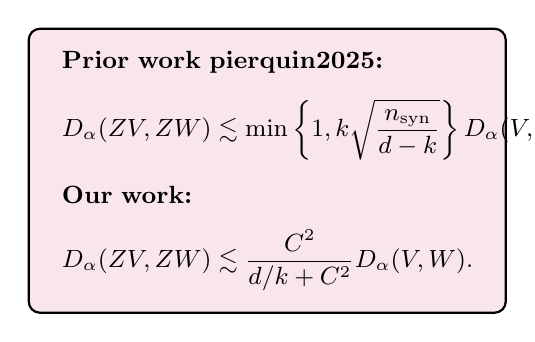
\begin{tikzpicture}
{\small
    \node[
      draw,                   % draw the border
      fill=purple!10,         % light purple background
      thick,                  % slightly thicker border line
      rounded corners,        % optional rounding
      inner xsep=12pt,        % horizontal padding
      inner ysep=8pt,         % vertical padding
      text width=0.43\textwidth,% wrap lines at 80% of text width
      align=left              % left-align text inside
    ] (mybox) {
      \textbf{Prior work~\citep{pierquin2025}:} 
     $$D_\alpha(ZV,ZW) \lesssim \min\left\{1, k\sqrt{\frac{n_{\text{syn}}}{d-k}}\right\}D_\alpha(V,W).$$
     \textbf{Our work:}
     $$D_\alpha(ZV,ZW) \lesssim \frac{C^2}{d/k + C^2} D_\alpha(V,W).$$
    };
    }
  \end{tikzpicture}
\caption{Summary of our results highlighting the improvements over prior work by \citet{pierquin2025}.}
\label{fig:summary}
\end{figure}



  
% $VZ$ and $WZ$ are two distributions of a family that can be parametrized by the mean of the left Gaussian matrix in the product ($v$ and $w$). We denote as $P_v$ the distribution of $VZ$ and $P_w$ the distribution of $WZ$. 


\section{Relationship between Fisher information and Rényi divergences}
\label{sec:fisher-renyi}
% This section addresses the main technical obstacle in our analysis:
This section presents some key technical results (some of which novel) that we will use to address our main goal:
upper bounding the privacy loss induced in the infinite synthetic data release regime ($n_{\text{syn}}\rightarrow+\infty$). Let $v,w \in \mathbb{R}^{d\times k}$ be the parameter produced by two adjacent datasets, with $\|v-w\|_F \leq \Delta$, and $P_v$ and $P_w$ the corresponding infinite release distributions of $ZV$ and $ZW$. Unfortunately, as we will see in Sections~\ref{sec:linear-regression} and~\ref{sec:multilinear-regression}, the Rényi divergence $D_\alpha(P_v, P_w)$ is generally intractable and does not admit simple bounds.

Instead of attempting a direct computation, we take an indirect approach. We embed the parameters $v$ and $w$ into a smooth parametric family $\{P_{\theta}, \theta \in \Theta\}$ that interpolate between $P_v$ and $P_w$, and we study the Fisher information of this family with respect to $\theta$. While still not directly computable, this quantity is typically more tractable to bound than the Rényi divergence itself. Then, we leverage a relationship between Rényi divergences and the Fisher information. Rényi divergences admit a local second-order expansion governed by Fisher information.

\begin{proposition}[Local relationship between Rényi divergences and Fisher information; \citealt{Haussler1997, vanErven2014}]
\label{prop:local-fisher}
    Let $\alpha > 1$. Let $P = \{P_\theta,\; \theta\in \Theta \subset \mathbb{R}\}$ be a family of probability distributions, with associated densities $p_\theta$. 
    For $\theta \in \Theta$, let the Fisher information $I(\theta) = \mathbb{E}_{X \sim P_\theta}[(\partial_\theta \log p_\theta(X))^2]$ and $\Delta > 0$. Then, under some regularity conditions (see Definition~\ref{defi:regularity}),
    \[D_\alpha(P_{\theta + \Delta},P_{\theta}) = \frac{\alpha}{2}I(\theta)\Delta^2 + o(\Delta^2).\]
\end{proposition}

The above proposition establishes an approximation of the Rényi divergence $D_\alpha(P_{\theta+\Delta},P_{\theta})$ in terms of the Fisher information $I(\theta)$. This result is particularly useful for families of distributions in which the Fisher information is substantially easier to compute than the Rényi divergence. However, this approximation is local, in the sense that it holds when the sensitivity $\Delta$ is small, and, to our knowledge, does not extend to global relationships between Rényi divergence and Fisher information. An existing attempt by \citet{Abbasnejad2006} contains a flaw in its proof; see Appendix~\ref{app:fisher-global-counterexample}, where we also clarify in Appendix~\ref{app:fisher-global-counterexample} why global comparison statements based on pointwise Rényi divergences and Fisher information cannot hold in general, and we give a basic counterexample.

For privacy certification, one requires \emph{non-asymptotic} upper bounds. In this work, we proceed by introducing an upper envelope $U$ on the Rényi divergence $D_{2\alpha-1}(P_z,P_\theta)$ along a path: $D_{2\alpha-1}(P_z,P_\theta)\leq U(z,\theta)$. Then, we show that for any such choice of $U$, a uniform bound on the Fisher information along the path yields a upper bound on Rényi divergence $D_\alpha(\theta',\theta)$. In particular, whenever $U$ is tractable, this provides a closed-form upper bound for $D_\alpha(\theta',\theta)$.

\begin{proposition}[Upper bounding Rényi divergences through Fisher information]
\label{prop:Fisher-upper-bound}
    Let $\theta < \theta' \in \Theta$ and $\alpha > 1$. We assume that there exists a function $U : \mathbb{R}^2 \to \mathbb{R^+}$ such that for all  $z \in (\theta,\theta')$, $D_{2\alpha-1}(P_{z},P_{\theta}) \leq U(z,\theta)$. We denote: \begin{align*}
        D_\theta^{\theta'} = \int_{\theta}^{\theta'} e^{(\alpha-1)U(z,\theta)}dz.
    \end{align*}  Then, under some regularity conditions (see Definition~\ref{defi:regularity}):
    \begin{align*}
        D_\alpha(P_{\theta'},P_{\theta}) \leq \frac{1}{\alpha-1}\log \bigg( 1 + \alpha \sup_{z \in (\theta,\theta')}I(z)^{1/2} D_\theta^{\theta'}\bigg).
    \end{align*}
\end{proposition}

A discussion about the tightness of this upper bound can be found in Appendix~\ref{app:prop-Fisher-upper-bound}. We note that related considerations and proof techniques appear in~\citet{Karbowski2024} to bound the rates of several statistical divergences under temporal evolution of the distributions. In contrast, Proposition~\ref{prop:Fisher-upper-bound} yields a global bound after integrating along a parameter path, provided a computable upper envelope $U$ of $D_{2\alpha-1}$ is available. %Without such control, the upper bound would be self-referential and vacuous.

In our setting, this condition follows from the post-processing inequality. In fact, as synthetic data is a randomized function of the parameters, we have $D_{2\alpha-1}(P_v,P_w)\leq   D_{2\alpha-1}(V,W)$, yielding a closed-form upper envelope. This allows us to control the Rényi divergence in terms of the Fisher information. Crucially, if the Fisher information is small along a path, the upper bound forces $D_\alpha(P_{\theta'},P_\theta)$ to be small, which we will leverage to prove privacy amplification.

In summary, we have obtained two complementary tools to characterize privacy amplification:
\begin{itemize}
    \item The local expansion in Proposition~\ref{prop:local-fisher} will yield sharp privacy amplification heuristics in regimes where the sensitivity $\Delta$ is small.
    \item The global, non-asymptotic bound of Proposition~\ref{prop:Fisher-upper-bound} ensures rigorous guarantees. We will use it to show that privacy amplification holds for every value of $\Delta$.
\end{itemize}

\section{From Outputs to Sufficient Gram Statistics}
\label{sec:sufficient}

As explained in Section~\ref{sec:l_infty}, our goal is to quantify the privacy loss $D_\alpha(ZV,ZW)$ associated to synthetic data release, especially when $n_{\mathrm{syn}}$ is large. In this section, we show that the test between $ZV$ and $ZW$ can be reduced to a test between $V^\top V$ and $W^\top W$ when $n_{\mathrm{syn}} \to +\infty$.
We first show the following result.

\begin{restatable}{proposition}{propSufficientStats}
\label{prop:sufficient-statistics}
    Assume $n_{\mathrm{syn}}\geq d\geq k$. Then,
    \[D_\alpha(ZV,ZW) = D_\alpha(V^\top Z^\top Z V, W^\top Z^\top Z W).\]
\end{restatable}
The proof, provided in Appendix~\ref{app:prop-sufficient-statistics}, relies on showing that the map $T : X \mapsto X^\top X$ is a sufficient statistic for distinguishing between $ZV$ and $ZW$. The matrix $Z^\top Z$ follows a Wishart distribution $\mathcal{W}(d,n_{\mathrm{syn}})$ with shape $d$ and degree of freedom $n_{\mathrm{syn}}$. Then, a careful analysis allows us to connect the divergence between $ZV$ and $ZW$ to the divergence between $V^\top V$ and $W^\top W$ in the asymptotic regime.

\begin{restatable}{proposition}{propGramLimit}
\label{prop:gram-limit}
    Assume $d \geq k$. Then,
    \[D_\alpha(V^\top Z^\top Z V, W^\top Z^\top Z W) \overset{n_{\mathrm{syn}}\to \infty}{\longrightarrow} D_\alpha(V^\top V, W^\top  W).\]
    Furthermore, for all $n_{\mathrm{syn}}> 1$, \[D_\alpha(ZV,ZW) \leq D_\alpha(V^\top V, W^\top  W).\]
\end{restatable}

This key proposition allows us to obtain privacy guarantees for any $n_{\mathrm{syn}} \in \mathbb{N}^*$ by analyzing $D_\alpha(V^\top V, W^\top  W)$. The limit depends on $V,W$ only through the Gram matrices $V^\top V$ and $W^\top W$. This reduction is the core technical simplification that unlocks closed-form upper bounds for the divergence. In particular $D_\alpha(V^\top V, W^\top  W)$ is the privacy loss associated to releasing an infinite amount of synthetic data. In other words, from a privacy perspective, \textbf{the release of arbitrarily many synthetic data is equivalent to releasing the Gram matrix $V^\top V$}. 

In the rest of the paper, we focus on deriving an upper bound for $D_\alpha(V^\top V, W^\top  W)$.
We first state a negative result: without additional assumptions, releasing infinitely many synthetic records provides no stronger privacy guarantees than releasing the generative model itself.
% there is no general privacy amplification compared to releasing the generative model when releasing an infinite amount of synthetic data without further assumption.

\begin{restatable}{proposition}{propNoFreeLunch}{\normalfont (No worst-case amplification in the $n_{\mathrm{syn}} \to + \infty$ regime).}
\label{prop:nofreelunch}
    \[\sup_{v,w \in \mathbb{R}^{d \times k}, \|v-w\|_F \leq \Delta}D_\alpha(V^\top V, W^\top  W) = D_\alpha(V,W).\]
\end{restatable}
The idea of the proof is to take $v_\theta = t e_1, w_t = (t + \Delta)e_1$, where $e_1 = (\delta_{11}) \in \mathbb{R}^{d\times k}$. As $t$ tends to $+\infty$, the matrices $V^\top V$ and $W^\top W$ diverge in a way that allows an adversary to recover $V$ and $W$.

To rule out this pathological behavior, we henceforth assume that the parameters are bounded.
\begin{assumption}[Parameter space boundedness]
    We assume that there exists $C > 0$ such that for any parameters $v,w$ obtained from adjacent datasets: \[\max\{\|v\|_F,\|w\|_F\} \leq C.\]
\end{assumption}
% Although essential for privacy amplification,
%  this requirement is mild in practice. In the regularized linear regression setting considered in this work, the weights are automatically bounded with an explicit constant $C$ (see Appendix [REF]).
We note that parameter boundedness is a standard assumption in the theory of private learning algorithms such as Projected Noisy Gradient Descent \citep{Feldman2018,Altschuler2022}.

% In the rest of the paper, we thus assume that $\|v\|_F, \|w\|_F \leq C$.



\section{Privacy Amplification in Linear Synthetic Data Generation}

In this section, we build on the results of Sections~\ref{sec:fisher-renyi} and~\ref{sec:sufficient} to derive our main privacy amplification guarantees for synthetic data generation with a linear generator.

\subsection{Releasing One-Dimensional Synthetic Data}
\label{sec:linear-regression}

We begin by analyzing the simpler case $k = 1$, which corresponds to releasing one-dimensional synthetic data points.
% (single-output) linear regression.
When $k=1$, $V^\top V= \|N+v\|^2$ and $W^\top W=\|N+w\|^2$ are scalar-valued non-central chi-squared random variables with the same degree of freedom $d$ and different non-centrality parameters $\|v\|^2,\|w\|^2$. We denote this distribution by $\chi_d^2(\theta^2)$, where $\theta^2$ is the non-centrality parameter. In particular, we have $V^\top V \sim \chi_d^2(\|v\|^2)$ and $W^\top W \sim \chi_d^2(\|w\|^2)$. The probability density function of $\chi_d^2(\|v\|^2)$ is given by:
\[p_v(x) = p_0(x)e^{- \|v\|^2/2} \|v\|^{1-d/2} I_{d/2-1}\big(\|v\| \sqrt{x}\big),\]
where $I_{d/2-1}$ is the modified Bessel function of the first kind with index $d/2-1$ and $p_0$ is the density of a central chi-squared distribution with degree of freedom $d$. We denote the family of non-central chi-squared distributions with respect to the amplitude parameter as \[P := \{p_\theta= \chi_d^2(\theta^2); \; \theta \in \mathbb{R^+}\},\] and the Fisher information associated with this family as $$I(d,\theta) := \mathbb{E}_{Y \sim p_\theta}[(\partial_\theta \log p_\theta)^2].$$


The Fisher information of non-central chi-squared distribution for the amplitude parameter is not available in closed form~\citep{Idier2014}. As a result, much of the literature has focused either on deriving lower bounds~\citep{Bouhrara2018, Idier2014, Stein2016} or on numerical estimation methods~\citep{Bouhrara2018}. The literature on upper bounds remains limited, aside from the work of~\citet{Idier2014} which proposes an upper bound for the Fisher information of generalized Rician distributions (more details in Appendix~\ref{app:fisher-one-dim}). In this section, we tighten the upper bound of~\citet{Idier2014}.



\begin{restatable}{proposition}{propFisherUpperBoundOneDim}\normalfont(Fisher information of non-central $\chi^2$).
\label{prop:Fisher-upper-bound-one-dim}
For all $\theta> 0, d > 2$ and  $p_\theta \in P$, and :
    \[\frac{2\theta^2}{2\theta^2 + d} \leq I(d,\theta) \leq \frac{2\theta^2}{2\theta^2 + d-3}.\]
\end{restatable}

This upper bound nearly matches the lower bound of \citet{Idier2014} reproduced in the proposition. Taken together, the two bounds tightly sandwich the Fisher information within the same functional form $2\theta^2/(2\theta^2 + d)$, up to a constant shift in the denominator. In particular, as noted for example by~\citet{Idier2014}, they capture the asymptotic behavior: \[I(d,\theta) \overset{d\to + \infty}{\longrightarrow} 0,\;\; I(d,\theta) \overset{\theta\to + \infty}{\longrightarrow} 1.\]
These bounds characterize the dependence of the Fisher information on both the degrees of freedom $d$ and the non-centrality parameter $\theta^2$. They will play a crucial role in deriving upper bounds on the Rényi divergence between non-central chi-squared distributions.


Using the Fisher information bounds derived above and the local comparison principle in Proposition~\ref{prop:local-fisher}, we can derive our first key result: explicit lower and upper bounds on the Rényi divergence $D_\alpha(V^\top V, W^\top W)$.

\begin{theorem}[Privacy amplification in the $n_{\mathrm{syn}} \to + \infty$ and % $n_{\mathrm{syn}} \to + \infty$
high privacy regime, $k=1$]
\label{thm:local-renyi}
    Assume without loss of generality that $\|w\|_F^2 \leq \|v\|_F^2 \leq C$. 
    % We note $m(C,d) = 2C^2/(2C^2 + d)$, $M(C,d) = 2C^2/(2C^2 + d-3)$, 
    We note the amplification factor:
    \[\eta_d = \frac{D_\alpha(V^\top V,W^\top W)}{D_\alpha(V,W)}.\]
    For $k=1$, we have:
    \begin{align*}
       \frac{2\|w\|^2}{2\|w\|^2 + d} + o(1) \leq \eta_d \leq \frac{2C^2}{2C^2 + d-3} + o(1),
    \end{align*}
    where the $o(1)$ term is relative to the sensitivity $\Delta$.
\end{theorem}
This result provides a sharp characterization of the divergence. The rightmost inequality shows that the divergence is upper bounded by the factor $2C^2/(2C^2 + d-3)$ that quantifies the degree of privacy amplification.

We observe two distinct behaviors. As $\|w\|, C \to +\infty$, the amplification factor lower bound $2C^2/(2C^2 + d)\to 1$, yielding no amplification, consistent with Proposition~\ref{prop:nofreelunch}. However, for a fixed $C > 0$, the amplification factor tends to $0$ at rate $O(d^{-1})$.  Importantly, the lower bound that we obtain shows that our analysis is sharp: this behavior is not an artifact of our proof technique. As a result, our upper bound provides a unified and tight expression capturing both amplification and post-processing. While this bound is only relevant when the sensitivity is small, this is typically the case if parameters are obtained through regularized linear regression, where $\Delta$ is of order $1/n$ \citep{chaudhuri2011differentiallyprivateempiricalrisk}. 

Nevertheless, we also derive a global upper bound based on our criterion in Proposition~\ref{prop:Fisher-upper-bound}.
\begin{restatable}{theorem}{thmUpperBoundRenyiOneDim}\normalfont (Privacy amplification in the $n_{\mathrm{syn}} \to + \infty$ regime, $k=1$).
\label{thm:upper-bound-renyi-one-dim}
Let us denote: \[f(\alpha, C,d,\Delta) = 1+\alpha \sqrt{\frac{2C^2}{2C^2 + d-3}}\frac{e^{(\alpha-1) (2\alpha-1) \frac{\Delta^2}{2}} -1}{(\alpha-1)(2\alpha-1)\Delta}.\]
 Then, for $k=1$, we have:
    \begin{align*}
        D_\alpha(V^\top V,W^\top W) 
        \leq \frac{1}{\alpha-1}\log f(\alpha,C,d,\Delta).
    \end{align*}
\end{restatable}

Due to our proof technique, we obtain a $o(d^{-1/2})$ rate, relying on the asymptotic equivalence $\log(1+x) \sim x$ when $d$ is small relative to the other considered quantities. However, Theorem~\ref{thm:local-renyi} suggests that a $o(d^{-1})$ exact rate is achievable. 


\subsection{Releasing Multi-Dimensional Synthetic Data}
\label{sec:multilinear-regression}


We now turn to the evaluation $D_\alpha(V^\top V, W^\top W)$ in the general case where $k>1$. In this multi-dimensional case, the matrix $V^\top V$ now follows a non-central Wishart distribution $\mathcal{W}(k,d,v^\top v)$ with size $k$, degree of freedom $d$ and non-centrality parameter $\Omega_v = v^\top v$. When $d \geq k$, $V^\top V$ admits a density~\citep{Muirhead2009}:
\[P_v(y) =  P_0(y) e^{-tr(\Omega_v)/2} {}_0F_1\Big(\frac{d}{2}, \frac{1}{4}y^{1/2} \Omega_v y^{1/2} \Big),\]
where $P_0$ denotes the density of the (central) Wishart distribution $\mathcal{W}(k,d)$ of size $k$ and with degree of freedom $d$, and ${}_0F_1$ is the generalized hypergeometric function of a matrix argument. The function ${}_0F_1$ can be characterized as a series involving zonal polynomials of a matrix argument. However, these latter polynomials are notoriously hard to handle~\citep{Koev2006}, making direct computation of $D_\alpha(V^\top V,W^\top W)$ intractable.
% We now consider the case $k > 1$, which corresponds to multi-output linear regression. In this case, $V^\top V$ follows a non-central Wishart distribution $\mathcal{W}(k,d,v^\top v)$ with size $k$, degree of freedom $d$ and non-centrality parameter $\Omega_v = v^\top v$. As discussed in Section~\ref{sec:fisher-renyi}, a direct computation of $D_\alpha(V^\top V,W^\top W)$ intractable.
Furthermore, the Fisher information upper bounds of Proposition~\ref{prop:Fisher-upper-bound-one-dim} do not readily extend to the $k>1$ setting. In fact, although the diagonal elements of $V^\top V$ are independent non-central chi-squared random variables, the non-diagonal elements are not independent, and follow a substantially more complex joint distribution. To our knowledge, there is no existing analysis in the literature characterizing the Fisher information of non-central Wishart distributions with respect to the non-centrality parameter.

Let $v = U_v^\top \Sigma_v S_v, w = U_w^\top \Sigma_w S_w$ denote the singular value decomposition of $v$ and $w$, and define the Gram operator $G(M) = M^\top M$. Leveraging the invariance of Gaussian matrices by orthogonal transformations, we obtain the following result.

\begin{lemma}[Rényi divergence equivalence along the SVD]
Let $G_v = G((N+\Sigma_v)S_v)$, $G_w = G((N+\Sigma_v)S_w)$. Then,
\[D_\alpha(V^\top V, W^\top W) = D_\alpha (G_v,G_w).\]
\end{lemma}

The distribution of $V^\top V$ is invariant under left multiplication of $v$ by orthogonal matrices. %Then, we can consider without loss of generality that $U_v = U_w$. However, note in general that $\|v-w\|_F \neq \|U_v v- U_w w\|_F$, and this discrepancy will be taken into account in the privacy analysis. 
Then, distinguishing between $V^\top V$ and $W^\top W$ is equivalent to distinguishing between between the corresponding non-centrality matrices $G(\Sigma_v)$ and $G(\Sigma_w S_w S_v^\top)$. In order to do this, we introduce a smooth parametrization between these two non-centralities and derive a upper bound on the associated Fisher information. This construction leverages the geometry  and the invariance of the non-centrality parameter:
$v \overset{(1-\theta) v + \theta U w}{\longrightarrow} w$, for any orthogonal matrix $U \in O(d)$.

Our analysis relies on the decomposition of $V^\top V = \sum_{i=1}^d V_i^\top V_i$ into a sum of independent non-central Wishart matrices. Then, we aggregate these terms into $\lfloor d/k \rfloor$ non-central Wishart matrices with rank $1$ non-centrality parameters. Coupled with a post-processing argument, this allows to relate the considered Fisher information to the Fisher information of non-central chi-squared distributions, which has been analyzed in Section~\ref{sec:linear-regression}.

Below, we get a upper bound of Fisher information for the straight line parametrization.


\begin{restatable}{theorem}{propFisherUpperBoundMultiDim}\normalfont (Fisher information of non-central Wishart distributions).
\label{prop:fisher-upper-bound-multi-dim}
Assume $d \geq k$. For $v,w \in \mathbb{R}^{d \times k}$, there exists a smooth path $\theta \in [0,1] \mapsto v_\theta \in \mathbb{R}^{d \times k}$ for the family of distributions: \[P := \{p_{\theta} = \mathcal{W}(k,d,v_\theta^\top v_\theta); \; \theta \in [0,1]\},\] such that $p_{0} = p_v$, $p_{1} = p_w$, and for all $\theta \in [0,1]$, the Fisher information $I(\theta)$ of the family of distribution $P$ with respect to  $\theta$ verifies: 
    \[I(\theta) \leq \inf_{U\in O(d)}\|v - U w\|_F^2  \frac{2\|v_\theta\|_F^2}{2\|v_\theta\|_F^2+ \lfloor d/k \rfloor - 3},\]
    with $\|v_\theta\|_F = \|(1-\theta) v + \theta Uw\|_F$.
\end{restatable}  

Using the Fisher information upper bound derived above and integrating along the path, we can upper bound the Rényi divergence using the general Fisher information criterion of Proposition~\ref{prop:Fisher-upper-bound}. Leveraging these results, we can upper bound the privacy loss associated to releasing an infinite number of synthetic data for $k>1$.
% multivariate linear regression setting.

\begin{restatable}{theorem}{thmUpperBoundRenyiMultiDim}{\normalfont (Privacy in the $n_{\mathrm{syn}} \to + \infty$ regime, $k>1$).} \label{thm:upper-bound-renyi-multiple-dim}Assume without loss of generality that $\|w\|_F ,\|v\|_F \leq C$. We note the amplification factor:
    \[\textstyle \eta_{d,k} = \frac{D_\alpha(V^\top V,W^\top W)}{D_\alpha(V,W)}.\]
    For $k>1$, we have:
    \begin{align*}
       & \eta_{d,k} \leq  \frac{2C^2}{2C^2 + \lfloor d/k \rfloor - 3}+ o(1),
    \end{align*}
    where the $o(1)$ term is relative to the sensitivity $\Delta$. 
    
    Moreover, we have the general upper bound:
    \[D_\alpha(V^\top V,W^\top W) \leq \frac{1}{\alpha-1}\log f(\alpha,C,\lfloor d/k \rfloor,\Delta).\]
\end{restatable}

This upper bound establishes a privacy amplification phenomenon for releasing $k$-dimensional synthetic data. The regime $d \geq k$ is practically relevant, as in many modern regimes, the model is overparametrized, with $d \gg k$.

\begin{remark}
     
    % The regime $d > k$ is practically relevant: in multivariate linear regression, one typically assumes $d > k$ to ensure that the (empirical) feature covariance is invertible, and in many modern regimes, the model is overparametrized, with $d \gg k$.
    We conjecture that our Fisher information upper bound is improvable. Some looseness might arise from our post-processing technique, which decomposes the non-centrality matrix into rank $1$ matrices. In particular, sharper Fisher information upper bounds might be obtained by leveraging the structure of the hypergeometric function of a matrix argument ${}_0F_1$. In Appendix~\ref{app:improvement-fisher-multiple}, we outline such an approach in the case $k=1$, providing an alternative proof of the Fisher information bound from Proposition~\ref{prop:Fisher-upper-bound-one-dim}, which we believe could be extended to non-central Wishart distributions. We then discuss the additional ingredients required to generalize the argument to the case $k>1$.
\end{remark}


\section{Experiments}
\label{sec:experiments}
In this section, we perform experiments to illustrate our theoretical results. While sampling from $ZV$ or $V^\top V$ is straightforward, their densities are analytically intractable. Therefore, we rely on variational inference methods to estimate the Rényi divergences. Specifically, we numerically estimate the privacy loss using the \emph{Convex-Conjugate Rényi Variational Formula}, introduced by~\citet[][(Theorem 2.1 therein]{birrell2023}. In order to estimate the Rényi divergence between two distributions $P$ and $Q$, we proceed as follows. We initialize a two-layer neural network $f(w_0,\cdot)$ with negative poly-softplus activation~\citep{birrell2023} and train it to maximize:
\[\sup_{w} \Big\{ \int f(w)dQ + \frac{1}{\alpha - 1} \log \int |f(w)|^{(\alpha-1)/\alpha} dP \Big\}.\]
Optimization is performed via minibatch stochastic gradient ascent. At each iteration, we sample $X = (X_1,\dots, X_l) \sim P^{\otimes l}$, $Y = (Y_1,\dots,Y_l) \sim Q^{\otimes l}$ for some batch size $l > 0$ and update the parameters using the empirical objective:
\begin{align*}
    F(w,X,Y) &= \textstyle\frac{1}{l}\sum_{i=1}^lf(w,Y_i)\\ & +  \textstyle\frac{1}{\alpha - 1}\log\Big(- \frac{1}{l}\sum_{i=1}^l f(w,X_i)^{(\alpha-1)/\alpha}\Big).
\end{align*}
A more detailed discussion can be found in Appendix~\ref{app:experiments}. 


\subsection{Estimating $D_\alpha(ZV,ZW)$ as a function of $n_{\text{syn}}$}
We estimate the divergence $D_\alpha(ZV,ZW)$ as a function of the number of released synthetic samples $n_{\text{syn}}$, in order to qualitatively assess its convergence behavior. Remarkably, Figure~\ref{fig:divergence-nsyn} shows that the Rényi divergence rapidly converges to a plateau, whose value is strictly lower than that of the corresponding post-processing privacy guarantee. Empirically, the number of synthetic samples required to reach the plateau appears to increase with $d$. The different values of the plateaus (dotted lines) highlight the amplification, which is significant even for the small values of $d \in (1,10)$ considered here. This empirical behavior illustrates our theoretical finding that privacy amplification persists under unlimited data release, and validates our focus on the infinite synthetic data release regime.
% This behavior is supported by theoretical analysis, as demonstrated in Section~\ref{subsec:convergence-rate}. 

\begin{figure}[h]
    \centering
    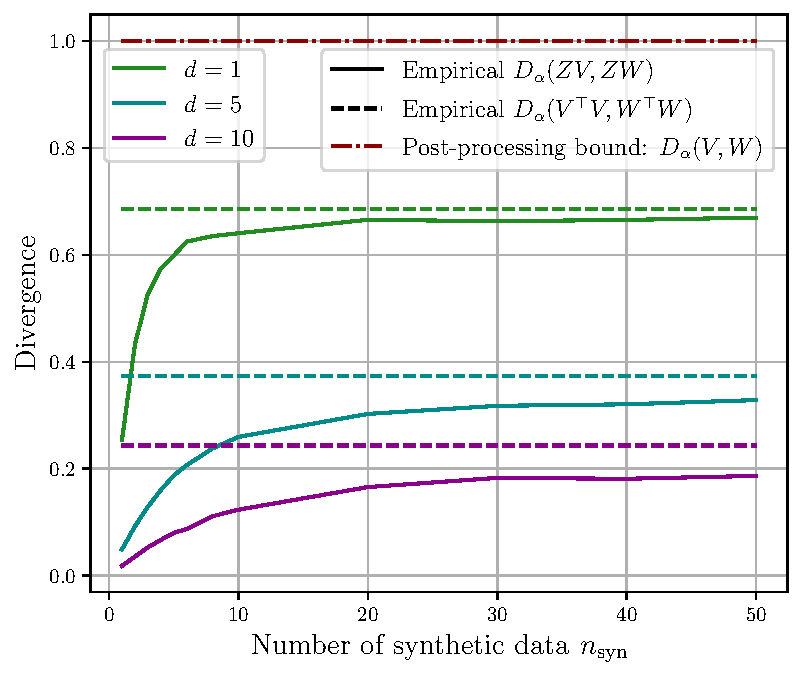
\includegraphics[width=.99\linewidth]{Divergencesyn.pdf}
    \caption{Empirical estimation of $D_\alpha(ZV,ZW)$ as a function of the number of released synthetic data $n_{\text{syn}}$ for multiple values of $d$, $k = \Delta = 1$, $C = \alpha = 2$.}
    \label{fig:divergence-nsyn}
\end{figure}



\subsection{Estimating $D_\alpha(V^\top V, W^\top W)$ as a function of $d,\Delta$}

In this section, we aim to estimate the empirical tightness of the local Rényi divergence bounds derived from Fisher information (Theorem~\ref{thm:local-renyi}) in the case where $k=1$. These bounds are asymptotic, and are thus expected to be informative only in the high privacy regime $\Delta \ll 1$. 
% Specifically, we consider the upper and lower bounds from Proposition~\ref{prop:Fisher-upper-bound-one-dim}:
% \[m(\|w\|_F, d) = \frac{2\|w\|_F^2}{2\|w\|_F^2 + d}, \;M(C,d) = \frac{2C^2}{2C^2 + d - 3}, \]
Specifically, we assess, for $\Delta \in (0,1)$, the extent to which the relation predicted by Theorem~\ref{thm:local-renyi} is satisfied: $2\|w\|_F^2/(2\|w\|_F^2 + d) \lesssim \eta_d \lesssim 2C^2/(2C^2 + d - 3)$. We estimate the Rényi divergence $D_\alpha(V^\top V, W^\top W)$  and compare the results to the theoretical envelope induced by the above bounds. In our experiments, we set $1\leq \|w\|_F \leq \|v\|_F \leq C = 2$, and evaluate $D_\alpha(V^\top V, W^\top W)$ as a function of $\Delta$. The results, represented in Figure~\ref{fig:fisher-delta}, show that for small perturbations ($\Delta < 1$), the theoretical local bounds provide an accurate estimation of the amplification. In particular, for $d=50$, the amplification effect is clearly observable.

\begin{figure}[h]
    \centering
    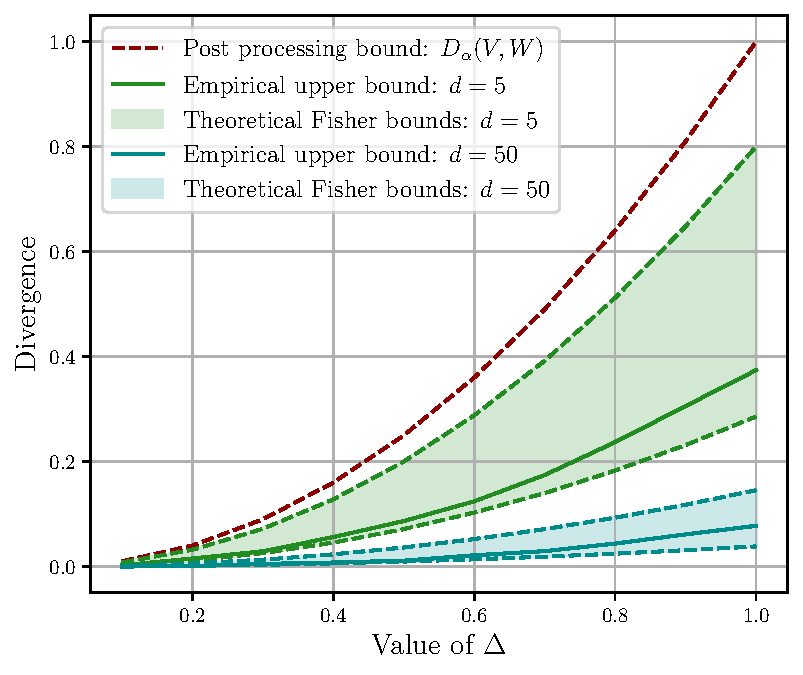
\includegraphics[width=.99\linewidth]{FisherDelta.pdf}
    \caption{Empirical estimation of $D_\alpha(V^\top V,W^\top W)$ as a function of $\Delta$ for multiple values of $d$, $k = 1$, $\|w\|_F \geq 1$, $C = 2$.}
    \label{fig:fisher-delta}
\end{figure}


\section{Discussion}

In this section, we discuss the tightness of the infinite data release privacy loss $D_\alpha(V^\top V, W^\top W)$ with respect to $D_\alpha(ZV,ZW)$. We also discuss potential directions for extending privacy amplification results to linear generators trained with widely used private learning algorithms.

\subsection{On the tightness of the plateau $D_\alpha(V^\top V, W^\top W)$}
\label{subsec:convergence-rate}
As discussed in Section~\ref{sec:experiments} and~\ref{sec:l_infty}, the privacy loss $D_\alpha(ZV,ZW)$ converges to $D_\alpha(V^\top V, W^\top W)$ when $n_{\text{syn}} \to +\infty$.
A natural question is whether the plateau $D_\alpha(V^\top V,W^\top W)$ is a meaningful approximation of $D_\alpha(ZV,ZW)$ for finite $n_{\text{syn}}$, especially when $d$ is large. %In fact, one possible worry is that for $n_{\text{syn}}$ fixed, the approximation becomes worse as $d$ increases, leaving a privacy gap unreachable by our analysis. 
We show that, in the tractable case $k=1$, for sufficiently large $d$,  the rate of convergence of the difference $D_\alpha(V^\top V, W^\top W) - D_\alpha(ZV,ZW)$ to $0$ is \textbf{at least} as fast as $O(1/n_{\text{syn}})$, with constants that can be chosen uniformly over all large $d$.


\begin{proposition}[Privacy gap is $O(1/n_{\text{syn}})$ for $k=1$]
\label{prop:privacy-gap}
     Let $\alpha \geq 2$ and $v,w \in \mathbb{R}^{d}$. Let $\tau = (\|v\|,\|w\|,\Delta,\alpha)$ and assume that $k=1$. Then, there exists $ K = K(\tau), K' = K'(\tau)$ and a threshold $d_0 = d_0(\tau)$ such that for all $d \geq d_0$ and $n_{\text{syn}} \geq 1$:
    \[\textstyle D_\alpha(V^\top V, W^\top W) - D_\alpha(ZV,ZW) \leq  \frac{K}{n_{\text{syn}}} + K' e^{-c n_{\text{syn}}}.\]
\end{proposition}

We are interested in regimes where $D_\alpha(V^\top V,W^\top W)$ itself decreases with $d$ (e.g., scaling like $d^{-\gamma}$ for some $\gamma > 0$, $\gamma \geq 1/2$ follows from Theorem~\ref{thm:upper-bound-renyi-multiple-dim}). In such regimes, the additive gap bound above can be used to assess tightness: achieving a constant-factor approximation of the plateau requires the gap to be smaller than the plateau scale.

\begin{corollary}[Constant factor tightness for large $n_{\text{syn}}$]
\label{corr:privacy-gap-scaling}
    Assume that $D_\alpha(V^\top V,W^\top W) = \Omega(d^{-\gamma})$, $k=1$. Then,  choosing $n_{\text{syn}}\gtrsim d^{\gamma}$ suffices to make $D_\alpha(ZV,ZW)$ a constant-factor approximation of the plateau (up to exponentially small terms).
\end{corollary}

A tighter characterization of the regime $n_{\text{syn}} \leq d$ than the work of~\citet{pierquin2025} is an interesting direction for future work, as it seems that some additional privacy gains may be achievable in this regime.

\begin{remark}
    The constants in Proposition~\ref{prop:privacy-gap} can be drastically improved by leveraging the fact that $D_\alpha(V^\top V, W^\top W) \lesssim d^{-\gamma} D_\alpha(V,W)$, as proved in Theorem~\ref{thm:upper-bound-renyi-multiple-dim}.
\end{remark}
\subsection{On the generalization to other training procedures}

The approach developed in this paper may extend to alternative training procedures for linear generators. Importantly, the sufficient-statistics limit  $D_\alpha(ZV,ZW) \overset{n_{\text{syn}} \to \infty}{\longrightarrow} D_\alpha(V^\top V, W^\top W)$ of Proposition~\ref{prop:sufficient-statistics} does not rely on $V$ or $W$ being isotropic Gaussian matrices (related to output perturbation). As noted by~\citet{Brown2024}, Noisy Gradient Descent applied to linear regression converges to a matrix Gaussian distribution, suggesting that our framework could naturally accommodate this more general setting. Extending the analysis in this direction is a promising avenue for future work.\looseness=-1

\section{Conclusion}

In this work, we studied privacy amplification for synthetic data released by a linear generator and showed that, under parameter boundedness, amplification persists even when releasing an unbounded number of synthetic samples. Our analysis provides a unified characterization of the privacy loss that smoothly interpolates between classical post-processing guarantees and genuine amplification. Notably, it does not depend on the number of released synthetic records, improving on the work of~\citet{pierquin2025}.

A key technical insight is that, in the infinite-release regime, the privacy loss is fully characterized by Gram statistics $V^\top V$, which enables tractable bounds via Fisher information. This yields local (high privacy) Rényi DP upper bounds with tight amplification factors. Beyond the local regime, we derived a general upper bound on Rényi divergence based on a criterion relating Fisher information to Rényi divergences provided a computable upper envelope on the Rényi divergence. While this bound is fully non-asymptotic and broadly applicable in our setting, we do not expect it to be tight in general. An important open question is whether this criterion can be improved to recover the local rates globally.

More broadly, our results provide concrete analytical insights, such as the role of parameter boundedness, the Fisher information analysis, the explicit dependence of amplification on the model dimension, and the sufficient statistics reduction. We expect that these insights will provide both intuition and methodological guidance for understanding privacy amplification in more complex models and data release mechanisms.

An important direction for future work in this regard is to extend these results to deep generative models trained with practical differentially private algorithms like DP-SGD, in order to determine whether similar privacy amplification phenomena manifest in realistic settings.

\section*{Impact Statement}

This paper presents work whose goal is to advance the field of Machine Learning. There are many potential societal consequences of our work, none which we feel must be specifically highlighted here.


\bibliography{references}
\bibliographystyle{apalike}

\newpage

%\clearpage
\appendix

\onecolumn


This appendix provides detailed discussions, proofs and supplementary content.
\section{Background on differential privacy}
 
\label{app:DP}
This section briefly reviews the differential privacy notions and tools used in the paper. Throughout, $\mathcal{M}$ denotes a randomized mechanism. We call two datasets $\mathcal{D}$ and $\mathcal{D}'$ of the same size $n$ \emph{adjacent} if they differ in exactly one data record.

Rényi Differential Privacy quantifies privacy via the Rényi divergence between the output distributions induced by $\mathcal{M}$ on adjacent datasets~\citep{Mironov2017}.
\begin{definition}[Rényi Differential Privacy (RDP)~\citep{Mironov2017}]
     For $\alpha>1, \varepsilon > 0$, the Rényi divergence of order $\alpha$ between distributions $P$ and $Q$ is $D_\alpha(P,Q) := \frac{1}{\alpha-1}\log\mathbb{E}_{x \sim P}\Big[\big(\frac{P(x)}{Q(x)}\big)^\alpha\Big]$. For $X \sim P, W \sim Q$, we note $D_\alpha(V,W) = D_\alpha(P,Q)$. Then, $\mathcal{M}$ satisfies $(\alpha,\varepsilon)$-RDP if for every pair of adjacent datasets $\mathcal{D},\mathcal{D}'$,
     \[D_\alpha(\mathcal{M}(\mathcal{D}) \| \mathcal{M}(\mathcal{D}')) \leq \varepsilon.\]
\end{definition}

The prior results of~\citet{pierquin2025} are formulated for trade-off functions in the $f$-Differential privacy ($f$-DP) framework. Trade-off functions~\citep{Dong2019} describe the optimal relationship between type I and type II errors for tests that attempt to distinguish the outputs produced from two adjacent datasets. Formally, let $P$ and $Q$ be two distributions and consider testing:
\[H_1: \text{the distribution is } P \text{~~ vs ~~} H_2: \text{the distribution is } Q.\]
For a  rejection rule $\phi\in[0,1]$, the type I error is $\mathbb{E}_P[\phi]$ and the type II error is $1-\mathbb{E}_Q[\phi]$.
\begin{definition}[Trade-off function]
    Let $t \in (0,1)$. Then, the trade-off function of the statistical test between $H_1$ and $H_2$ is defined as:
    \[T(P,Q)(t) = \inf_{\phi} \{1-\mathbb{E}_Q[\phi]:\mathbb{E}_P[\phi] \leq t\}.\]
    For $X \sim P, W \sim Q$, we note $T(V,W) = T(P,Q)$.
\end{definition}

$f$-Differential privacy is defined as a upper bound condition on the function $f$ for any trade-off function between the statistical test between adjacent datasets:
\[H_1: \text{the distribution is } \mathcal{M}(\mathcal{D}) \text{~~ vs ~~} H_2: \text{the distribution is } \mathcal{M}(\mathcal{D}').\]

\begin{definition}
    Let $f:[0,1]\to[0,1]$ be a decreasing convex function. A mechanism $\mathcal{M}$ satisfies \emph{$f$-differential privacy} ($f$-DP) if for all adjacent datasets $\mathcal{D},\mathcal{D}'$,
    \[T(\mathcal{M}(\mathcal{D}),\mathcal{M}(\mathcal{D}')) \geq f.\]
\end{definition}
\section{Comparison of our upper bounds to the prior results of~\citet{pierquin2025}}
\label{app:comparison-prior-work}
In Section~\ref{sec:l_infty}, we mentioned that the privacy loss upper bounds obtained by~\citet{pierquin2025} follow the relationship:
\[D_\alpha(ZV,ZW) \lesssim \min\left\{1, k\sqrt{\frac{n_{\text{syn}}}{d-k}}\right\}D_\alpha(V,W).\]

We clarify that this upper bound is not a guarantee offered by~\citet{pierquin2025} (after conversion from trade-off functions to RDP). It represents the best \emph{best scaling} one can hope to extract from their proof technique. This means that any conversion of the results of~\citet{pierquin2025} to RDP guarantees is at least as loose as this bound. In the rest of the section, we make precise this claim and highlight several limitations of these guarantees. 

The privacy loss upper bounds of~\citet{pierquin2025} are formulated in terms of trade-off functions. We restate below the result we use, with the notational change that the trade-off function argument is denoted by $t\in(0,1)$ (reserving $\alpha$ for Rényi orders).
\begin{theorem}[Privacy amplification for synthetic data, adapted from~\citep{pierquin2025}]
\label{theo:convergence-trade-off-multi-dim}

    Let $d > 0$. We denote $C_{n_{\text{syn}},k,d} =  C'k \sqrt{\frac{n_{\text{syn}}}{d-k}}$, where $C' > 0$ is an absolute constant. Let $N \in \mathbb{R}^{n_{\text{syn}} \times d}$ be a Gaussian matrix independent of $Z$, and define the trade-off function: \[G_{(d-k,v,w)} = T\left(\sqrt{d-k}N + Zv,  \sqrt{d-k}N + Zw\right),\]
    with $G_{(d-k,v,w)}(t) = 0$ for $t > 1$.
    
    Then, for all $t \in (0,1)$:
    \begin{equation}
    \label{equa:prior-tf-bound}
        f:=\max\left\{T(V,W),G_{(d-k,v,w)}\left(t + C_{n_{\text{syn}},k,d}\right) -C_{n_{\text{syn}},k,d}\right\} \leq T(ZV,ZW)(t).
    \end{equation}
\end{theorem}

Specifically, we show that:
\begin{itemize}
    \item Proposition~\ref{prop:prior-dp-delta}: Any $(\varepsilon,\delta)$-DP conversion of the amplification term $G_{(d-k,v,w)}\left(t + C_{n_{\text{syn}},k,d}\right) -C_{n_{\text{syn}},k,d}$ of Equation~\ref{equa:prior-tf-bound} yields $\delta = \Omega\left(k(n_{\text{syn}}/d)^{1/2}\right)$. In particular, to get $\delta = o(n^{-1})$ (with $n$ the sample size), one would need $n_\text{syn} = o\left(\frac{d}{k^2 n^2}\right)$.
    \item Proposition~\ref{prop:prior-no-amplification}: Equation~\ref{equa:prior-tf-bound} does not yield any amplification in the high privacy regime $\Delta  < 2C'k \sqrt{\frac{2\pi n_{\text{syn}}}{d-k}}$. In this regime, the privacy loss is no better than $D_\alpha(V,W)$. 
    \item Proposition~\ref{prop:prior-rate}: In the privacy amplification regime, the Rényi divergence conversion $l_\alpha(f)$ of the trade-off function $f$ derived from Equation~\ref{equa:prior-tf-bound} scales as $2C'k \sqrt{\frac{ n_{\text{syn}}}{d-k}}$: \[l_\alpha(f) \geq 2C'k \sqrt{\frac{ n_{\text{syn}}}{d-k}} D_\alpha(V,W).\]
\end{itemize}

First, we explain our proof strategy to derive RDP bounds from Equation~\ref{equa:prior-tf-bound}. Figure~\ref{fig:lower-tradeoff-function} represents the associated trade-off function. This function is piecewise, separated into two regions: a Gaussian trade-off region and an amplification region. By symmetry, the trade-off function is Gaussian at the edges, in the set $(0,x_-)\cup (x_+,1)$ for some $0 \leq x_- \leq x_+ \leq 1$, and $G_{(d-k,v,w)}\left(t +  C_{n_{\text{syn}},k,d}\right) -C_{n_{\text{syn}},k,d}$ at the center, in the interval $(x_-,x_+)$. Then, Propositions~\ref{prop:prior-dp-delta} and~\ref{prop:prior-no-amplification} become clear: any $(\varepsilon,\delta)$ conversion of the amplification regime yields $\delta \geq C_{n_{\text{syn}},k,d}$. Moreover, there is no amplification if the curve $G_{(d-k,v,w)}\left(t + C_{n_{\text{syn}},k,d}\right) -C_{n_{\text{syn}},k,d}$ does not intersect the curve $T(V,W)$. We identify the regimes where it happens.

\begin{figure}[h]
    \centering
    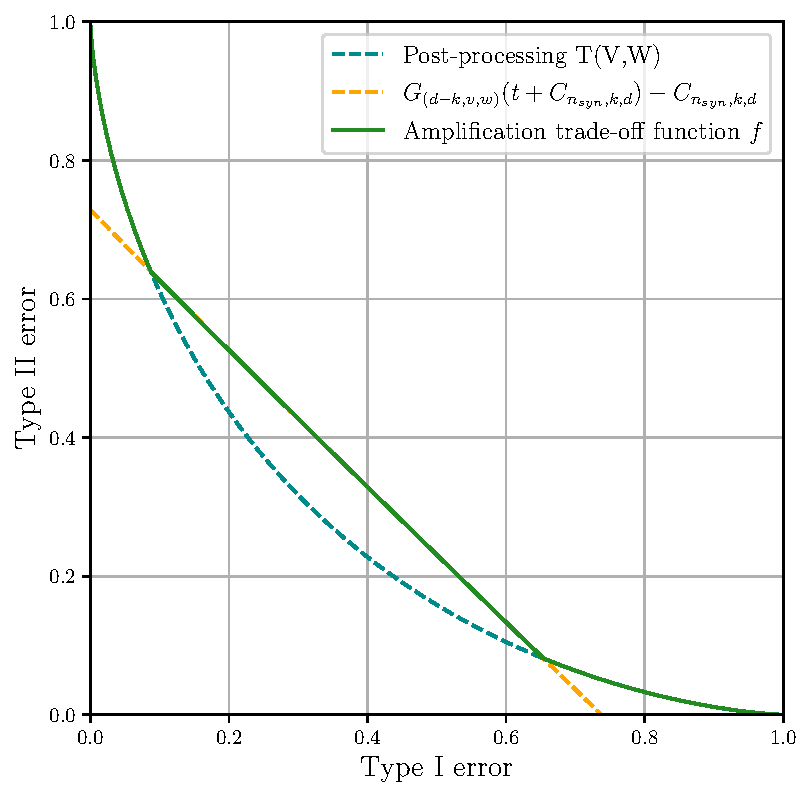
\includegraphics[width=0.4\linewidth]{tradeOffFunction.pdf}
    \caption{Representation of the trade-off function $f$ for $\Delta=1, C' = 1, d = 60, n_{\text{syn}} = 1, k=1$.}
    \label{fig:lower-tradeoff-function}
\end{figure}

\textbf{Relaxing the trade-off function $f$}:
We rely on a simplification of the $G_{(d-k,v,w)}\left(t + C_{n_{\text{syn}},k,d}\right) -C_{n_{\text{syn}},k,d}$ part. Let $t \in (0,1)$. From Equation~\ref{equa:prior-tf-bound}, $T(ZV,ZW)(t) \geq f(t)$. $f$ is the certifiable privacy loss upper bound obtained by~\citet{pierquin2025}. Then, for any trade-off function $h > f$, the analysis of~\citet{pierquin2025} is not sufficient to certify privacy. In particular, any trade-off function $T$ satisfies $T(t) \leq 1-t$. As $G_{(d-k,v,w)}$ is a trade-off function, we have $G_{(d-k,v,w)} \leq 1- I_d$. Then, \[f \leq \max\left\{T(V,W),1-I_d - 2C_{n_{\text{syn}},k,d}\right\} = \max\left\{\Phi(\Phi^{-1}(1-\alpha) - \Delta),1-I_d - 2C_{n_{\text{syn}},k,d}\right\} := g,\]  where $\Phi$ is the Gaussian cumulative distribution function.

Replacing $G_{(d-k,v,w)}\left(t + C_{n_{\text{syn}},k,d}\right) -C_{n_{\text{syn}},k,d}$ by $1-I_d - 2C_{n_{\text{syn}},k,d}$ unlocks simpler Rényi divergence conversion. This yields lower bounds and minimal conditions for amplification. 

\textbf{A useful reparametrization}: Now, assume that the curves $\Phi(\Phi^{-1}(1-\cdot )$ and $1-I_d - 2C_{n_{\text{syn}},k,d}$ intersect (which means that there is amplification). Note $z  = \Phi^{-1}(1-t)$. Then, $f(z) = \max\{\Phi(z - \Delta), \Phi(z) - 2C_{n_{\text{syn}},k,d}\}$. The intersection is located at the solutions of $\Phi(z) - \Phi(z-\Delta) = 2C_{n_{\text{syn}},k,d}$. We note $z_- \leq 0 \leq z_+$ the lower and upper solutions. 

\textbf{Converting trade-off function into RDP guarantees}:
From~\citet{Dong2019}, trade-off functions convert into Rényi divergences through the following functional:

\begin{proposition}[Conversion from $f$-DP to RDP~\cite{Dong2019}]
If a mechanism is $f$-DP, then it is $(\alpha,l_\alpha(f))$-RDP for all $\alpha >1$ with:
\[l_\alpha(f) = \begin{cases}
    \frac{1}{\alpha-1}\log \int |f'(t)|^{1-\alpha} dt \text{ if } z_f=1,\\ +\infty \text{ else,}
\end{cases}\]
with $z_f = \inf\{t \in (0,1); f(t) = 0\} =1$.
\end{proposition}

We can now prove Propositions~\ref{prop:prior-dp-delta},~\ref{prop:prior-no-amplification} and~\ref{prop:prior-rate}:


\begin{proposition}[DP conversion forces $\delta$ of order $C_{n_{\text{syn}},k,d}$]
\label{prop:prior-dp-delta}
Any $(\varepsilon,\delta)$-DP guarantee derived from the amplification part of Equation~\ref{equa:prior-tf-bound}
necessarily satisfies $\delta=\Omega(C_{n_{\text{syn}},k,d})$ (uniformly over $\varepsilon > 0$). Therefore, $n_\text{syn} = o\left(\frac{d}{k^2 n^2}\right)$.
\end{proposition}

\begin{proof}
    Immediate from the form of the trade-off function and the $(\varepsilon,\delta)$ conversion result of~\citet{Dong2019}. Therefore, for a reasonable privacy protection $\delta = o(n^{-1})$, we have $n^{-1} > C_{n_{\text{syn}},k,d}$, giving the desired result. Moreover, converting the trade-off function of Equation~\ref{equa:prior-tf-bound} either yields no amplification (in the Gaussian region) or large $\delta$ (in the amplification region).
\end{proof}

\begin{proposition}[No amplification in the high-privacy regimes]
\label{prop:prior-no-amplification}
If $\Delta < 2C'k \sqrt{\frac{2\pi n_{\text{syn}}}{d-k}}$, the RDP conversion $l_\alpha(f)$ of Equation~\ref{equa:prior-tf-bound} yields $l_\alpha(f) = D_\alpha(V,W)$. In particular, $G_{(d-k,v,w)}\left(t + C_{n_{\text{syn}},k,d}\right) -C_{n_{\text{syn}},k,d}$ does not intersect $T(V,W)$.
\end{proposition}

\begin{proof}
The function $H = \Phi(z) - \Phi(z-\Delta)$ is symmetric around $\Delta/2$. In fact,
\begin{align*}
    H\left(\frac{\Delta}{2} + z\right) &= P\left(N \leq \frac{\Delta}{2} + z\right) - P\left(N \leq z - \frac{\Delta}{2} \right)\\
     &= P\left(N \geq -\frac{\Delta}{2} - z\right) - P\left(N \geq - z + \frac{\Delta}{2} \right)\\
     &=  P\left(N \leq \frac{\Delta}{2} - z \right) - P\left(N \leq -\frac{\Delta}{2} - z\right)= H\left(\frac{\Delta}{2} - z\right).
\end{align*}
It is also increasing then decreasing. In fact, $H'(z) = \frac{1}{\sqrt{2\pi}}(e^{-z^2/2} - e^{-(z-\Delta)^2/2}) \geq 0 \iff z \leq \frac{\Delta}{2}$.
Its maximum value is attained for $z = \frac{\Delta}{2}$. Therefore, the intersection between $\Phi(\Phi^{-1}(1-t) - \Delta)$ and $ (1-t - 2C_{n_{\text{syn}},k,d})$ exists if and only if $H(\Delta/2) \geq 2C_{n_{\text{syn}},k,d}$.

Also, $H(\Delta/2) = \Phi(\Delta/2) - \Phi(-\Delta/2) = 2\Phi(\Delta/2)-1$.

Then, there is no amplification for:
\[2C_{n_{\text{syn}},k,d} > \frac{\Delta}{\sqrt{2\pi}} \geq \sqrt{\frac{2}{\pi}}\int_0^{\Delta/2} e^{-t^2/2} dt = 2\Phi(\Delta/2) -1.\]
\end{proof}

Now, we show that the conversion of the trade-off function $f$ into Rényi divergence $l_\alpha(f)$ satisfies $l_\alpha(f) \geq C_{n_{\text{syn}},k,d} D_\alpha(V,W)$ when $C_{n_{\text{syn}},k,d}$ is sufficiently small.


\begin{proposition}
\label{prop:prior-rate}
    Assume that $d > n_{\text{syn}}, k$. Then, in the privacy amplification regime, or equivalently, when $G_{(d-k,v,w)}\left(t + C_{n_{\text{syn}},k,d}\right) -C_{n_{\text{syn}},k,d}$ intersects with $T(V,W)$, the following relationship holds:
    \[l_\alpha(f) \geq 2C'k\sqrt{\frac{n_{\text{syn}}}{d-k}}D_\alpha(V,W).\]
\end{proposition}

\begin{proof}

We give a lower bound of the Rényi divergence associated to the trade-off function $f$. We decompose the integral into $3$ pieces representing the Gaussian regime and the amplification regime, and perform the change of variable $z = \Phi^{-1}(1-t)$.
\begin{align*}
    \exp((\alpha-1)l_\alpha(f)) &=  \int_0^1 |f'(t)|^{1-\alpha} dt\\ &=  \int_0^1 |\partial_\theta\max\left\{\Phi(\Phi^{-1}(1-t) - \Delta),1-t - C_{n_{\text{syn}},k,d}\right\}|^{1-\alpha} dt\\
    &=  \int_0^{1-\Phi(z_+)} |\partial_\theta \Phi(\Phi^{-1}(1-t) - \Delta)|^{1-\alpha}dt \\&+ \int_{1-\Phi(z_-)}^1  |\partial_\theta \Phi(\Phi^{-1}(1-t) - \Delta)|^{1-\alpha}dt + |\Phi(z_-) - \Phi(z_+)|\\
    &=  \int_0^{1-\Phi(z_+)}-(\Phi^{-1})'(1-t)^{1-\alpha} \phi(\Phi^{-1}(1-t) - \Delta)^{1-\alpha}dt \\&+ \int_{1-\Phi(z_-)}^1 -(\Phi^{-1})'(1-t)^{1-\alpha}\phi(\Phi^{-1}(1-t) - \Delta)^{1-\alpha}dt +|\Phi(z_-) - \Phi(z_+)|\\
    &= \int_{z_+}^{+\infty} \frac{\phi(z)^{\alpha}}{\phi(z-\Delta)^{\alpha-1}}dz + \int_{-\infty}^{z_-} \frac{\phi(z)^{\alpha}}{\phi(z-\Delta)^{\alpha-1}}dz +|\Phi(z_-) - \Phi(z_+)|\;,\; (z = \Phi^{-1}(1-t)),
\end{align*}
where $\phi$ is the Gaussian density function. By completing the square, for $x < y$, we have:
\begin{align*}
    \int_{x}^{y} \frac{\phi(z)^{\alpha}}{\phi(z-\Delta)^{\alpha-1}}dz &= \frac{1}{\sqrt{2\pi}}\int_{x}^{y} e^{((\alpha-1)(z-\Delta)^2-\alpha z^2)/2}dz\\
    &= \frac{1}{\sqrt{2\pi}}\int_{x}^{y} e^{(-z^2 -2(\alpha-1)\Delta + (\alpha-1)\Delta^2)/2}dz\\
    &= \frac{1}{\sqrt{2\pi}}\int_{x}^{y} e^{-(z + (\alpha-1)\Delta)^2)/2}dz\\
    &=\frac{1}{\sqrt{2\pi}}e^{\alpha(\alpha-1)\Delta^2/2}\int_{x}^{y} e^{(-z^2 -2(\alpha-1)\Delta + (\alpha-1)\Delta^2)/2}dz\\
    &= e^{\alpha(\alpha-1)\Delta^2/2} (\Phi(y + (\alpha-1)\Delta) - \Phi(x + (\alpha-1)\Delta)).
\end{align*}

Then, we can express $\exp((\alpha-1)l_\alpha(f))$ as a function of the Gaussian cumulative function distribution $\Phi$:
\begin{align*}
    \exp((\alpha-1)l_\alpha(f)) &= e^{\alpha(\alpha-1)\Delta^2/2} (1 - \Phi(z_+ + (\alpha-1)\Delta) + \Phi(z_- + (\alpha-1)\Delta)+ |\Phi(z_-) - \Phi(z_+)|\\
    &= e^{\alpha(\alpha-1)\Delta^2/2} (\Phi(z_- + (\alpha-1)\Delta) +\Phi(-(z_+ + (\alpha-1)\Delta)) +  \Phi(z_+) - \Phi(z_-)
\end{align*}

Now, we derive a upper bound to $\Phi(z_+) - \Phi(z_-)$. We note $G_\Delta : x \mapsto \Phi(\Phi^{-1}(1-x) - \Delta)$, and $x_+ = 1-\Phi(z_+), x_- = 1- \Phi(z_-)$. By symmetry of $G_\Delta$ ($G_\Delta = G_\Delta^{-1}$), $x_+ = G_\Delta(x_-)$ and, since $x_-$ is at the intersection between $G_\Delta$ and $1 - I_d - 2C_{n_{\text{syn}},k,d}$:
\[x_+ + x_- = G_\Delta(x_-) + x_- = 1 - 2C_{n_{\text{syn}},k,d}.\]

Also, leveraging the definitions of $x_-$ and $x_+$:
\[\Phi(z_+) + \Phi(z_-) = (1-x_+) + (1-x_-) = 1+2C_{n_{\text{syn}},k,d}.\]

Then, we show that $z_+ = z_- + \Delta$. In fact, $\Phi(z_+) - \Phi(z_+-\Delta) = 2C_{n_{\text{syn}},k,d}$ and: 
\begin{align*}
    \Phi(\Delta - z_+) - \Phi(-z_+) = \Phi(z_+) - \Phi(z_+ - \Delta) = 2C_{n_{\text{syn}},k,d}.
\end{align*}
Then, if $z$ is a solution of the equation $\Phi(z) - \Phi(z-\Delta) = 2C_{n_{\text{syn}},k,d}$ , $\Delta-z$ is also a solution of the equation. Since this equation only admits two solutions, $z_+ + z_- = \Delta$.
We note $A = \Phi(z_- + (\alpha-1)\Delta) +\Phi(-(z_+ + (\alpha-1)\Delta)$ and $L = \Phi(z_+) - \Phi(z_-)$. Then, we have shown that:
\begin{align*}
        \exp((\alpha-1)l_\alpha(f)) &= e^{\alpha(\alpha-1)\Delta^2/2} A+ L.
\end{align*}
Now, let us get a lower bound of this expression. Since $\Phi$ is increasing and $\alpha > 1$, we have:
\begin{align*}
    A = \Phi(z_- + (\alpha-1)\Delta) +\Phi(-(z_+ + (\alpha-1)\Delta) \geq \Phi(z_- + (\alpha-1)\Delta) \geq \Phi(z_-)  \geq 2C_{n_{\text{syn}},k,d}.
\end{align*}
Also, we obtain a lower bound of $A+L$ by showing that $(\Phi(z_- + (\alpha-1)\Delta)- \Phi(z_-)) -(\Phi(z_+ + (\alpha-1)\Delta) - \Phi(z_+)) \geq 0$.
\begin{align*}
    A+L &= 1+ (\Phi(z_- + (\alpha-1)\Delta)- \Phi(z_-)) -(\Phi(z_+ + (\alpha-1)\Delta) - \Phi(z_+))\\
    &= 1+ \int_{0}^{ (\alpha-1)\Delta} (\phi(t+z_-) -  \phi(t+z_+)) dt\\
    &= 1+ \frac{1}{\sqrt{2\pi}}\int_{0}^{ (\alpha-1)\Delta} e^{((t+z_+)^2 - (t+z_-)^2)/2} dt\\
    &= 1+ \frac{1}{\sqrt{2\pi}}\int_{0}^{ (\alpha-1)\Delta} e^{(z_+-z_-)(z_+ + z_- + 2t)/2} dt \geq 1.\\
\end{align*}
By the same reasoning,
\[0 \leq A = 1+ \Phi(z_- + (\alpha-1)\Delta) -\Phi(z_+ + (\alpha-1)\Delta) = 1 + \int_{z_+}^{z_-} \phi(t + (\alpha-1)\Delta) dt \leq 1.\]

Then, by convexity of the $x \mapsto e^x$ function for the input $A \alpha(\alpha-1)\Delta^2/2 + (1-A)\cdot 0$:
\[e^{\alpha(\alpha-1)\Delta^2/2} A+ L \geq e^{\alpha(\alpha-1)\Delta^2/2} A+ 1-A \geq e^{A\alpha(\alpha-1)\Delta^2/2} \geq  e^{C_{n_{\text{syn}},k,d}\alpha(\alpha-1)\Delta^2}.\]
Recall that $D_\alpha(V,W) = \alpha\Delta^2/2$. Then, 
\[\exp((\alpha-1)l_\alpha(f)) \geq \exp(2(\alpha-1) C_{n_{\text{syn}},k,d} D_\alpha(V,W)).\]
Then, the desired result holds:
\[l_\alpha(f) \geq 2C'k\sqrt{\frac{n_{\text{syn}}}{d-k}}D_\alpha(V,W).\]
\end{proof}

\newpage
\section{Relationship between Rényi divergences and Fisher information}
\label{app:Renyi-Fisher}

In this section, we introduce Fisher information and its properties needed for the understanding of the paper. Then, we examine the relationship between Rényi divergences and Fisher information.

\subsection{Fisher information and its properties}
\label{app:Fisher-properties}
This appendix briefly recalls the notion of Fisher information and the few properties we rely on throughout the paper. In this paper, we focus on Fisher information of families of probabilities indexed by scalar parameters. In this paper, all considered distributions are "sufficiently regular". We define sufficient regularity conditions for the usual Fisher information properties to hold.
\begin{definition}[Regular family of probability measures]
\label{defi:regularity}
     Let $P = \{P_\theta : \theta\in\Theta \subset \mathbb{R}\}$ be a family of probability measures on $(\mathbb{R},\mathcal{B}(\mathbb{R}))$. Then, $P$ is regular if:
     \begin{itemize}
         \item $\Theta$ is a right-open set of $\mathbb{R}$: for every point $\theta \in \Theta$, there exists a neighborhood of the form $[\theta,\theta + \delta) \subset \Theta$.
         \item All $P_\theta \in P$ have a common support.
         \item For all $\theta \in \Theta$, $P_\theta$ is absolutely continuous with respect to the Lebesgue measure. We note the corresponding densities $p_\theta$.
         \item For all $\theta \in \Theta$, $\theta \mapsto \log p_\theta(x)$ is twice almost everywhere differentiable.
         \item For all $\theta \in \Theta$,  there exist a neighborhood $U$ and integrable functions $\tilde h_1, \tilde h_2$ such that for all $\theta' \in U$, \[\left|\partial_{\theta'} p_{\theta'}(x)\right| \leq \tilde h_1(x), \;\; \left|\partial_{\theta'}^2 p_{\theta'}(x)\right| \leq \tilde h_2(x).\]
         This condition ensures the sufficient regularity of $P$ for generic properties of Fisher information to hold.
         \item For all $\theta \in \Theta$,  there exist a neighborhood $U$ and integrable functions $h_1, h_2$ such that for all $\theta' \in U$, \[\left|\partial_{\theta'}\log p_{\theta'}(x)\right|\frac{p_{\theta'}(x)^\alpha}{p_{\theta}(x)^{\alpha-1}} \leq h_1(x), \;\; \left(\partial_{\theta'} \log p_{\theta'} (x)^2 +\left| \partial_{\theta'}^2\log p_{\theta'}(x)\right|\right)\frac{p_{\theta'}(x)^\alpha}{p_{\theta}(x)^{\alpha-1}} \leq h_2(x).\]
         This condition is specific to the differentiability of Rényi divergences.
     \end{itemize}
\end{definition}
Note that these are not minimal conditions for the existence of Fisher information. Now, we define Fisher information and score functions:

\begin{definition}[Fisher information and score function]
    Let $P = \{P_\theta : \theta\in\Theta \subset \mathbb{R}\}$ be a regular family of probability measures. Then, the score function is defined by:
    \[s_\theta(x) = \partial_\theta \log p_\theta(x).\]
    The Fisher information of the family $P$ with respect to the parameter $\theta \in \Theta$ is:
    \[I(\theta) = \mathbb{E}_{X \sim P_\theta}[s_\theta(X)^2] \in \mathbb{R}^+.\]
\end{definition}

Here are some properties of the Fisher information that are used throughout the paper:

\begin{proposition}[Fisher information and score properties]
\label{prop:Fisher-properties}
    Let $P = \{P_\theta : \theta\in\Theta \subset \mathbb{R}\}$ be regular of probability  measures such that the Fisher information $I(\theta)$ exists for all $\theta \in \Theta$. Then, the Fisher information and the score function satisfy the following properties:
    \begin{itemize}
        \item \textbf{Mean-zero score and information identity, Lemma 5.3 of~\citet{Lehmann1998}:} $\mathbb{E}_{X \sim P_\theta}[s_\theta(X)] = 0$, hence $I(\theta) = \Var_{X \sim P_\theta}(s_\theta(X))$. Moreover, when $\partial_\theta^2 \log p_\theta(X)$ exists almost averywhere, the information identity holds: \[I(\theta) = - \mathbb{E}_{X \sim P_\theta}[\partial_\theta^2 \log p_\theta(X)].\]
        \item \textbf{Post-processing inequality~\citep{Schervish1995}:} Let $X\sim P_\theta$ and let $Y \sim K(X)$ be generated from a Markov kernel $K$ applied on $X$. Then, \[I_Y(\theta) \leq I_X(\theta).\]
        \item \textbf{Additivity under independent products, adapted from Theorem 5.8 of~\citet{Lehmann1998}:} If $X = (X_1,\dots,X_n)$ are jointly independent given $\theta$, with joint density $p_\theta(x_1,\dots,x_m)=\prod_{i=1}^n p^{(i)}_\theta(x_i)$, then the Fisher information of $X$ with respect to the parameter $\theta$ decomposes as: \[I_{(X_1,\dots,X_n)}(\theta) = \sum_{i=1}^n I_{X_i}(\theta).\]
    \end{itemize}
\end{proposition}

\subsection{A local relationship between Rényi divergences and Fisher information}
\label{app:Local-fisher-renyi}
In parametric distributions, the second order derivative of most $f$-divergences coincide the Fisher information~\citep{Polyanskiy2025}. Rényi divergences are obtained as a smooth monotone transformation of a $f$-divergence. This yields a local expansion of the second order of Rényi divergences as a function of Fisher information under small perturbations of the parameter for sufficiently regular families of distributions, as noted by~\citet{Haussler1997} and~\citet{vanErven2014}. However, in these works, the exact technical conditions on the parametrization that are needed are not explicited, and the authors do not know references for these conditions~\citep{vanErven2014}. For completeness, we prove that under the regularity conditions of Definition~\ref{defi:regularity}, the local expansion of Rényi divergences as a function of Fisher information hold. In this paper, all considered families of distributions satisfy these conditions. Note that we do not claim that these conditions are minimal.

\begin{proposition}[Local relationship between Rényi divergences and Fisher information]
\label{prop:local-fisher-app}
    Let $\{P_\theta, \theta\in \Theta \subset \mathbb{R}\}$ be a family of probability distributions. 
    Let $\theta \in \Theta$. Let $\Delta > 0$ such that $\theta + \Delta \in \Theta$. Then, if $P$ is regular (Definition~\ref{defi:regularity}),
    \[D_\alpha(P_{\theta + \Delta},P_{\theta}) = \frac{\alpha}{2}I(\theta)\Delta^2 + o(\Delta^2).\]
\end{proposition}

\begin{proof}
    Let $\alpha > 1$ and $P$ be a regular family of distribution, as defined in Definition~\ref{defi:regularity}. For $\theta,\theta' \in \Theta$, we note $H(\theta',\theta) = \int \frac{p_{\theta'}(x)^\alpha}{p_{\theta}(x)^{\alpha-1}} dx$. Fix $\theta \in \Theta$ and note for every $\theta' \in \Theta$, $G(\theta') = H(p_{\theta'}, p_{\theta})$. Let $\Delta > 0$ such that $\theta + \Delta \in \Theta$. Since $P$ is regular, the conditions of Definition~\ref{defi:regularity} are sufficient to ensure the twice differentiability of $G$. Then $G(\theta) = 1$ and:
    \begin{align*}
        \partial_{\theta'} G(\theta') &= \alpha\int \partial_{\theta'} \log p_{\theta'} (x)\frac{p_{\theta'}(x)^\alpha}{p_{\theta}(x)^{\alpha-1}} dx,\\
        \partial_{\theta'}^2 G(\theta') &= \alpha \int (\partial_{\theta'}^2\log p_{\theta'}(x) + \alpha (\partial_{\theta'} \log p_{\theta'}(x))^2)\frac{p_{\theta'}(x)^\alpha}{p_{\theta}(x)^{\alpha-1}} dx.
    \end{align*}
    Since score has mean $0$ (Proposition~\ref{prop:Fisher-properties}), $\partial_{\theta} G(\theta) = 0$ and $\partial_{\theta}^2 G(\theta) = \alpha \mathbb{E}_{X \sim P_\theta}[\partial_\theta^2 \log p_\theta(X)] + \alpha^2 I(\theta)$. By the information equality (Proposition~\ref{prop:Fisher-properties}), $I(\theta) = -\mathbb{E}_{X \sim P_\theta}[\partial_\theta^2 \log p_\theta(X)]$. Therefore, $\partial_\theta^2 G(\theta) = \alpha (\alpha-1) I(\theta)$.
    Since $G$ is positive and twice differentiable on $\Theta$, $D : \theta' \mapsto D_\alpha(P_{\theta'}, P_\theta) = \frac{1}{\alpha-1} \log G(\theta')$ is twice differentiable on $\Theta$. Then,
    \begin{align*}
        \partial_{\theta'} D(\theta') &= \frac{1}{\alpha-1} \frac{\partial_{\theta'} G(\theta')}{G(\theta')},\\
        \partial_{\theta'}^2 D(\theta') &= \frac{1}{\alpha-1} \left(\frac{\partial_{\theta'}^2 G(\theta')}{G(\theta')} - \frac{\partial_{\theta'} G(\theta')^2}{G(\theta')^2}\right).
    \end{align*}
    Therefore, $\partial_\theta D(\theta) = 0$ and $\partial_\theta^2 D(\theta) = \alpha I(\theta)$.
    Thus, the following asymptotic expansion holds:
     \[D_\alpha(P_{\theta + \Delta},P_{\theta}) = \frac{\alpha}{2}I(\theta)\Delta^2 + o(\Delta^2).\]
\end{proof}

\subsection{Beyond the local expansion: can Fisher information control Rényi divergence globally?}
\label{app:fisher-global-counterexample}

A natural question is whether this local relationship between Fisher information and Rényi divergences extends beyond infinitesimal perturbations. More precisely, one may ask if there is a \emph{distribution-free} functional $F$ such that, given an arbitrary regular family of distribution $P$ and any $\theta < \theta' \in \Theta$:  \[D_\alpha(P_{\theta'}, P_\theta) = F(\alpha, \{I(u); \;u \in [\theta,\theta']\}).\] In general, no such characterization exists: Fisher information is a local quantity, and it does not determine Rényi divergence for arbitrary parameter values. Our counterexample of Theorem 4.1 of~\citet{Abbasnejad2006}, studied below, is a simple illustration of two family distributions that can have the same Fisher information but different Rényi divergences. There are, however, specific families of distributions in which global formulas are available. First, for distributions belonging to the same exponential family, Fisher information~\citep[Theorem~5.4]{Lehmann1998} and Rényi divergences~\citep[Chapter~2]{Liese1987} admit a closed form. Specific choices of parameters yield an integral representation of Rényi divergences in terms of the Fisher information~\citep{Bercher2012}, but these parametrizations do not simplify the theoretical calculation of the associated Rényi divergences, as the ratio $\frac{p_{\theta'}(x)^t}{p_{\theta}(x)^{1-t}}$ $(t \in (0,\alpha))$ appear in the parametrized densities.


A different line of work attempts to obtain global comparison criterions. For instance, one may hope that pointwise ordering of Fisher information implies ordering of Rényi divergences:
\[\text{ For all }\; \theta \in \Theta,\; I_P(\theta) \leq I_Q(\theta) \implies \text{For all } \theta < \theta' \in \Theta,\; D_\alpha(P_{\theta'},P_\theta) \leq D_\alpha(Q_{\theta'},Q_\theta),\]
where $P$ and $Q$ are two families of distributions indexed by the same parameter set $\Theta$, and the corresponding Fisher information are $I_P$ and $I_Q$.

Two existing attempts in the literature for Rényi divergences~\citep[Theorem~4.1]{Abbasnejad2006} and Kullback-Leibler (KL) divergences~\citep[Theorem~3.1]{Habibi2006} obtain such a statement. However, but they are false in general, even for smooth regular families. We provide a counterexample and discuss the flaw in the proofs below.

\begin{theorem}[Adapted from Theorem 4.1 of~\citet{Abbasnejad2006}]
\label{thm:renyi-fisher-comparison-wrong}
Let $P = \{P_\theta,\ \theta\in \Theta\}$ and $Q = \{Q_\theta,\ \theta\in \Theta\}$ be two families of distributions. Let $0 < \theta_0 < \theta_1 \in \Theta$. Let $\alpha > 1$. Assume that both families have finite Rényi divergence and Fisher information, continuous in $\theta$. If the following conditions hold:
\begin{enumerate}
    \item \label{item:condition-1} For all $\theta \in I=[\theta_0,\theta_1], \;I_P(\theta) - I_Q(\theta) \geq d_0 > 0$,
    \item \label{item:condition-2} For all $\theta \in (\theta_0,\theta_1)$, $\delta \mapsto D_\alpha(p_{\theta + \delta},p_\theta)$ and $\delta \mapsto D_\alpha(q_{\theta + \delta},q_\theta)$ are three times differentiable and the third derivatives are uniformly bounded in a neighborhood $I = [0,c]$ of zero, then:
\end{enumerate}
\[ D_\alpha(p_{\theta_1},p_{\theta_0}) >D_\alpha(q_{\theta_1},q_{\theta_0}).\]
\end{theorem}
We start by pointing a counterexample to this theorem.

\paragraph{Counterexample of Theorem 4.1 from~\citet{Abbasnejad2006}:}
Fix $\alpha = 2$. Let $a, \sigma > 0$. Let $P_a = \{ \Cauchy(\theta, a),\; \theta \in \mathbb{R}\}$, where $\theta$ is the location parameter of the Cauchy distribution and $a$ is the scale parameter, and $Q_\sigma = \{ \mathcal{N}(\theta, \sigma^2),\; \theta \in \mathbb{R}\}$. Let $\theta_0 < \theta < \theta_1 \in \mathbb{R}$. Then, for the location parameter the Fisher information is constant for both families:
\[I_{P_a}(\theta) = \frac{1}{2 a^2},\;\;\; I_{Q_\sigma}(\theta) = \frac{1}{\sigma^2}.\]
 Also, the Rényi divergence between Cauchy distributions~\citep{Verdu2023} and between Gaussian distributions is known:
 \[D_2(p_{\theta_1}, p_{\theta_0}) = \log\left(1 + \frac{(\theta_1-\theta_0)^2}{2 a^2}\right),\;\;\; D_2(q_{\theta_1}, q_{\theta_0}) = \frac{(\theta_1-\theta_0)^2}{\sigma^2}.\]
 Both families of distributions satisfy the condition~\ref{item:condition-2} of Theorem~\ref{thm:renyi-fisher-comparison-wrong}. Moreover, choosing $a < \frac{1}{\sqrt{2}}\sigma$ allows to satisfy the condition~\ref{item:condition-1}: for all $\theta \in [\theta_0,\theta_1]$, $I_{Q_\sigma}(\theta) \leq I_{P_a}(\theta)$.
 However, for sufficiently large values of $\theta_1 - \theta_0$, it is clear that $D_2(p_{\theta_1}, p_{\theta_0}) \leq D_2(q_{\theta_1}, q_{\theta_0})$.

\paragraph{Flaw in the proofs of Theorem 4.1 from~\citet{Abbasnejad2006} and Theorem 3.1 from~\citet{Habibi2006}:}
The core idea of~\citet{Abbasnejad2006} and~\citet{Habibi2006} relies on showing that, under condition~\ref{item:condition-1}, for all $\theta \in \Theta$, there exists $\delta, d_1 > 0$ such that $\frac{1}{\delta^2}(D_\alpha(p_{\theta + \delta}, p_\theta) - D_\alpha(q_{\theta + \delta}, q_\theta)) \geq d_1$. Then, they incorrectly drop the $1/\delta^2$, by stating that when $c < 1$ (so that $\delta < 1$), $D_\alpha(p_{\theta + \delta}, p_\theta) - D_\alpha(q_{\theta + \delta}, q_\theta) \geq d_1$, which is generally false. The proof is not fixable independently of the regularity conditions. In fact, they try to generalize this statement for larger values of $\delta$ by induction to derive a lower bound on $D_\alpha(p_{\theta + k\delta}, p_\theta) - D_\alpha(q_{\theta + k\delta}, q_\theta)$ for $k > 1$, by a telescoping argument, but now that the lower bound of $D_\alpha(p_{\theta + \delta}, p_\theta) - D_\alpha(q_{\theta + \delta}, q_\theta)$ depends on $\delta$, which depends on $\theta$, the recurrence fails.

The theorem of~\citet{Habibi2006} for KL divergence follows the same proof technique and is also false.





\subsection{A sufficient condition to control Rényi divergence with Fisher information (Proposition~\ref{prop:Fisher-upper-bound})}
\label{app:prop-Fisher-upper-bound}



In this section, we introduce a criterion that allows to obtain a upper bound of Rényi divergences as a function of Fisher information along a parameter segment $[\theta,\theta']$. The derivation assumes an explicit upper envelope on the Rényi divergence that is available in our setting. It has the desirable property that it vanishes when the Fisher information becomes small on $[\theta,\theta']$ (provided $D_{2\alpha-1}$ remains controlled). This upper bound is generally not tight, as it scales as $\sqrt{I(\theta)}$ when the Fisher information is small, while the the local expansion of Theorem~\ref{thm:local-renyi} suggests a $I(\theta)$ rate. Here is the statement of the criterion:

\begin{proposition}[Upper bounding Rényi divergences through Fisher information]
\label{prop:app-renyi-criterion}
    Let $\{P_\theta, \theta\in \Theta \subset \mathbb{R}\}$ be a family of distributions. Let $\theta < \theta' \in \Theta$.  We assume that there exists a function $U : \mathbb{R}^2 \to \mathbb{R^+}$ such that for all  $z \in (\theta,\theta')$, $D_{2\alpha-1}(P_{z},P_{\theta}) \leq U(z,\theta)$. We also assume that $z \mapsto D_\alpha(P_z,P_\theta)$ is differentiable on $(\theta,\theta')$.  Then,
    \[D_\alpha(P_{\theta'}, P_\theta) \leq \frac{1}{\alpha-1}\log \left( 1+ \alpha\sup_{z \in (\theta,\theta')} \sqrt{I(z)} \int_{\theta}^{\theta'} e^{(\alpha-1)U(z,\theta)}dz\right).\]
\end{proposition}

\begin{proof}
    For $\theta,\theta' \in \Theta$, we note $H(\theta',\theta) = \int \frac{p_{\theta'}(x)^\alpha}{p_{\theta}(x)^{\alpha-1}} dx$. Fix $\theta \in \Theta$ and note for every $\theta' \in \Theta$, $G(\theta') = H(p_{\theta'}, p_{\theta})$.

    Then, by Cauchy-Scharz inequality: 
    \begin{align*}
        \partial_{\theta'} G(\theta') &= \alpha\int \partial_{\theta'} \log p_{\theta'}(x) \frac{P_{\theta'}(x)^\alpha}{P_\theta(x)^{1-\alpha}}  dx\\
        &= \alpha\; \mathbb{E}_{X \sim P_{\theta'}} \left[\partial_{\theta'} \log p_{\theta'}(X) \left( \frac{P_{\theta'}}{P_\theta}\right)^{\alpha-1}\right]\\
        &\leq \alpha\; (\mathbb{E}_{X \sim P_{\theta'}} \left[(\partial_{\theta'}\log p_{\theta'}(X))^2\right])^{1/2}\left(\mathbb{E}_{X \sim P_{\theta'}} \left[\left( \frac{P_{\theta'}}{P_\theta}\right)^{2(\alpha-1)}\right]\right)^{1/2}\\
        &\leq \alpha \sqrt{I(\theta')}e^{(\alpha-1) D_{2\alpha-1}(P_{\theta '},P_\theta)}\\
        &\leq \alpha\sup_{z\in (\theta,\theta')} \sqrt{I(z)} e^{(\alpha-1) U(\theta',\theta)}.
    \end{align*}

    Integrating over $(\theta,\theta')$, we get:

    \[G(\theta') = G(\theta) + \int_{\theta}^{\theta'} \partial_{z} G(z) dz \leq 1+ \alpha\sup_{z \in (\theta,\theta')} \sqrt{I(z)} \int_{\theta}^{\theta'} e^{(\alpha-1)U(z ,\theta)}dz,\]
    giving the desired result.

\end{proof}

This upper bound can be directly leveraged in our setting. In fact, the Rényi divergence $D_{2\alpha-1}(ZV,ZW)$ is upper bounded by post-processing: $D_{2\alpha-1}(V^\top V,W^\top W) \leq D_{2\alpha-1}(V,W)$. Therefore, for any choice of parametrization of $V^\top V$, we can obtain a upper bound of $D_{2\alpha-1}(V^\top V, W^\top W)$ as a function of the post-processing upper bound and the Fisher information related to this parametrization.

As a validation step, we can compare this upper bound to the exact Rényi divergence in the case of the Rényi divergence between Gaussian distributions: $D_\alpha(N+z,N+w) = \frac{\alpha}{2 \sigma^2}(z-w)^2$, and the Fisher information is $I(z) = \frac{1}{\sigma^2}$.
Then, 
\begin{align*}
    D_\alpha(N+v,N+w) &\leq \frac{1}{\alpha-1} \log \left( 1+ \frac{\alpha}{\sigma} \int e^{(\alpha-1)(2\alpha-1) \frac{(z-w)^2}{2\sigma^2}}dz\right) \\
    &\leq \frac{1}{\alpha-1} \log \left( 1+ \frac{2\alpha \sigma}{(\alpha-1)(2\alpha-1)(v-w)} \left(e^{(\alpha-1)(2\alpha-1) \frac{(v-w)^2}{2\sigma^2}}-1\right)\right)
\end{align*}
Figure~\ref{fig:tightness-fisher-gaussian} represent the upper bound and the original divergence in the case $\sigma = 1, \alpha=2$, as a function of $\Delta$.
\begin{figure}[h]
    \centering
    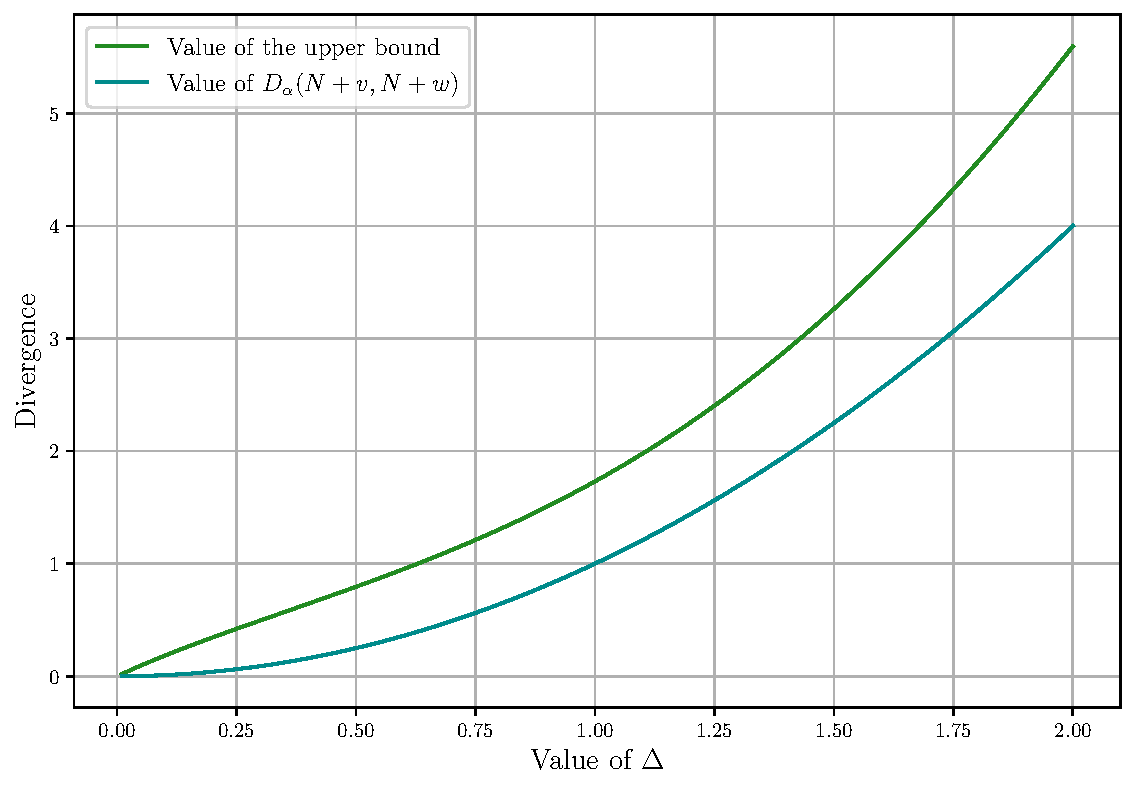
\includegraphics[width=0.5\linewidth]{tightnessFisherUpperGaussian.pdf}
    \caption{Comparison between the Rényi divergence $D_\alpha(N+v,N+w)$ and the criterion obtained from Proposition~\ref{prop:Fisher-upper-bound} as a function of $\Delta$, in the case $\sigma=1, \alpha = 2$.}
    \label{fig:tightness-fisher-gaussian}
\end{figure}


\newpage

\section{From Outputs to Sufficient Gram Statistics}

\subsection{Proof of Proposition~\ref{prop:sufficient-statistics}}
\label{app:prop-sufficient-statistics}
\propSufficientStats*

\begin{proof}
    For $n_{\text{syn}} \geq d \geq k$, the distributions of $ZV$ admits a density, which is a mixture of matrix normal distributions: $ZV | V=v \sim \mathcal{MN}_{n_{\text{syn}} \times k} (0, 0, v^T v)$. The density writes:
    \begin{align*}
        p_{ZV}(y) = \int  p(v) p_{Zv}(y) dv &= \int  p_V(v) (2\pi)^{- n_{\text{syn}} k /2} \det\left(v^\top v\right)^{-n_{\text{syn}}/2} \exp\left(-\frac{1}{2} \tr\left((v^\top v)^{-1}y^\top y\right)\right) dv\\
    \end{align*}
    Now, define $g_v(z) = \int  p_V(v) (2\pi)^{- n_{\text{syn}} k /2} \det\left(v^\top v\right)^{-n_{\text{syn}}/2} \exp\left(-\frac{1}{2} \tr\left((v^\top v)^{-1} z\right)\right) dv$. Then, \[p_{ZV}(y) = g_v(y^\top y) , \; p_{ZW}(y) = g_w(y^\top y).\]
    By the Fisher–Neyman factorization theorem, 
    \[D_\alpha(ZV,ZW) = D_\alpha(V^\top Z^\top Z V, W^\top Z^\top Z W).\]
\end{proof}

\subsection{Proof of Proposition~\ref{prop:gram-limit}}
\label{app:prop-gram-limit}

\propGramLimit*

\begin{proof}
First, observe that \[\frac{1}{n_{\text{syn}}}Z^\top Z = \frac{1}{n_{\text{syn}}}\sum_{i=1}^{n_{\text{syn}}} Z_i^\top Z_i \overset{n_{\text{syn}} \to \infty}{\to} I_d,\]
by the law of large numbers. This means that $\frac{1}{n_{\text{syn}}}V^\top Z^\top ZV \to V^\top V, \frac{1}{n_{\text{syn}}} W^\top Z^\top Z W \to W^\top W $.
    Also, Rényi divergences are lower semi-continuous for the weak topology~\citep{vanErven2014}.
    This means that:
    \[ \underset{n_{\text{syn}} \to \infty}{\lim} \inf D_\alpha(V^\top Z^\top Z V, W^\top Z^\top Z W) = \underset{n_{\text{syn}} \to \infty}{\lim} \inf D_\alpha\left(\frac{1}{n_{\text{syn}}}V^\top Z^\top Z V, \frac{1}{n_{\text{syn}}}W^\top Z^\top Z W\right) \geq D_\alpha(V^\top V, W^\top W).\]

    Also, we define the kernel $K : \Sigma_v \mapsto \frac{1}{n_{\text{syn}}}\mathcal{W}(k,n_{\text{syn}},\Sigma_v)$, for $\Sigma_v \in \mathbb{S}_k^+(\mathbb{R})$, or equivalently: $K(\Sigma_v) = \Sigma_v^{1/2} G^\top G \Sigma_v^{1/2}$.
    
    Now, we note $\Sigma_v = V^\top V$. Then, $V$ admits a polar decomposition $V = U_v \Sigma_v^{1/2}$, where $U \in \mathbb{R}^{d \times k}$ verifies $U_v^\top U_v = I_k$. Let $G \in \mathbb{R}^{n_{\text{syn}} \times k}$ be a standard Gaussian matrix. By invariance of Gaussian matrices by isometries, $ZV = ZU_v \Sigma_v^{1/2} \overset{d}{=} G\Sigma_v^{1/2}$, and:
    \begin{align*}
        D_\alpha(V^\top V, W^\top W) \geq D_\alpha(K(V^\top V), K(W^\top W)) &= D_\alpha\left(\Sigma_v^{1/2}G^\top G \Sigma_v^{1/2}, \Sigma_w^{1/2}G^\top G \Sigma_w^{1/2} \right)\\
        &= D_\alpha\left(V^\top U_v^\top Z^\top Z U_v V, W^\top U_w^\top Z^\top Z U_w W \right)\\
        &= D_\alpha\left(V^\top Z^\top Z V, W^\top Z^\top Z W \right).
    \end{align*}
    Finally, 
\[D_\alpha(V^\top Z^\top Z V, W^\top Z^\top Z W)\leq  D_\alpha(V^\top V, W^\top W) \leq \underset{n_{\text{syn}} \to \infty}{\lim} \inf D_\alpha(V^\top Z^\top Z V, W^\top Z^\top Z W),\]
giving the desired result.
\end{proof}



\newpage

\subsection{Proof of Proposition~\ref{prop:nofreelunch}}
\label{app:prop-nofreelunch}

\propNoFreeLunch*

\begin{proof}
    The idea of the proof is to take $v_\theta = t e_1, w_t = (t + \Delta)e_1$, where $e_1 = (\delta_{11}) \in \mathbb{R}^{d\times k}$. We note $V_t = N + v_t$ and $W_t = N + w_t$.
    % First, as proved in Lemma~\ref{lem:sufficient-stat-one-dim}, since $v_\theta$ is rank $1$,
    % \[D_\alpha(v_\theta^\top v_\theta,W_t^\top W_t) = D_\alpha(\chi_d^2(t^2),\chi_d^2(t+\Delta)^2)\]
    First, by post-processing:
    \[D_\alpha(V_t^\top V_t,W_t^\top W_t) \geq D_\alpha((V_t^\top V_t)_{11}, (W_t^\top W_t)_{11})) = D_\alpha(\chi_d^2(t^2),\chi_d^2((t+\Delta)^2)).\]
    Now, take $f : x \mapsto \sqrt{|x|}$. As $t \to \infty$, $f$ becomes injective on a set of probability $p_t \to 1$. The distribution of $f(\chi_d^2(t^2))$ converges weakly to $\mathcal{N}(t,1)$. Then, for all $t > 0$:
    \[\underset{t \to \infty}{\lim} \inf D_\alpha(f(\chi_d^2(t)),f(\chi_d^2((t + \Delta)^2)) \geq D_\alpha(\mathcal{N}(t,1), \mathcal{N}(t+\Delta, 1)) = D_\alpha(V,W),\]
    which is finite, giving the desired result.
\end{proof}

\section{Privacy amplification in linear regression}

\subsection{Computing the Fisher information of $\chi_d^2(\theta^2)$ for the amplitude parameter $\theta$}
\label{app:fisher-one-dim}

In this section, we restate the introduction of Section~\ref{sec:linear-regression} and add relevant results and details. The Fisher information of non-central chi-squared distribution for the amplitude parameter does not seem tractable~\citep{Idier2014}. As a result, most of the literature have focused either on deriving lower bounds~\citep{Bouhrara2018, Idier2014, Stein2016} or on numerical estimation~\citep{Bouhrara2018}. In contrast, the literature on upper bounds remains limited, aside from the trivial post-processing inequality $I(d,\theta) \leq 1$. 

In the work \citep{Idier2014}, authors focus on the Fisher information of Rician and generalized Rician distributions with respect to the amplitude parameter $\theta$. Generalized Rician distributions $R(\alpha, \theta)$ reduce to non-central chi distribution when the scale parameter $\alpha = 1$ or equivalently, to square root of non-central chi-squared random variables. Denoting $I_X(d,\theta)$ the Fisher information of generalized Rician distributions for the parameter $\theta$, and noting that $x \mapsto \sqrt{x}$ is bijective, we have $I(d,\theta) = I_X(d,\theta)$.
Then, computing a upper bound for $I_X(d,\theta)$ also give a upper bound to $I(\theta)$.

\citet{Idier2014} find the following upper bound:
\[I_X(d,\theta) \leq \min\left\{1,\frac{2\theta^2}{d}\right\}.\]
While useful in the $d \gg \theta^2$ regime, this bound is piecewise and does not naturally capture the asymptotic behaviour $I_X(d,\theta) \overset{\theta \to +\infty}{\to} 1$. In this section, we propose a tighter upper bound to $I_X(\theta)$, and therefore to $I(d,\theta)$ by leveraging the properties of the modified Bessel function of first kind $I_d$.

\begin{proposition}[Fisher information of non-central $\chi_d^2$, adapted from~\citet{Idier2014}]
\label{prop:FisherIdier}
    Let $d > 1$. Then, the Fisher information admits the representation:
    \[I_X(\theta) = \mathbb{E}_{Y \sim \mathcal{R}_{d/2,\theta}}[Y (R_{d/2-1}(Y) - R_{d/2}(Y))],\]
    where $R_d = \frac{I_{d+1}}{I_d}$ is the modified Bessel quotient of the first kind and $\mathcal{R}_{d/2,\theta}$ is a generalized Rician distribution with non-centrality parameter $\theta^2$, scale $\theta$ and degree $d/2$~\citep{Idier2014}: 
    \[\mathcal{R}_{d/2,\theta}(y) = \frac{y^{d/2+1}}{\theta^{d+2}} e^{-\frac{y^2 }{2\theta^2} - \theta^2/2} I_{d/2}(y).\]
\end{proposition}

Motivated by this characterization, we seek to improve upon the upper bounds of~\citet{Idier2014} by deriving a sharp upper bound on $Y (R_{d/2-1}(Y) - R_{d/2}(Y))$:

\begin{lemma}
\label{lem:bessel-upper-bound}
    Let $d > 2, x > 0$. Then,
    \[x(R_{d-1}(x) - R_{d}(x)) \leq \frac{x R_{d-1}(x)}{x R_{d-1}(x) + d -\frac{1}{2}}.\]
\end{lemma}

\begin{proof}
We note $R_d(x) = \frac{I_{d+1}(x)}{I_{d}(x)}$ the modified Bessel quotient of the first kind.
The modified Bessel functions of first kind admit the following recurrence relations~\citep[11.115~and~11.116]{Arfken2011}:
    \[I_{d-1}(x) - I_{d+1}(x) = \frac{2d}{x}I_d(x).\]
    \[I_{d-1}(x) + I_{d+1}(x) = 2 I_d'(x).\]

    Then, we relate $x (R_{d-1}(x) - R_{d}(x))$ to $I_{d}(x)^2-I_{d+1}(x)I_{d-1}(x)$: \begin{align*}
        x (R_{d-1}(x) - R_{d}(x)) &= x \left( \frac{I_{d}(x)}{I_{d-1}(x)} - \frac{I_{d+1}(x)}{I_{d}(x)} \right)\\
        &=x  \frac{I_{d}(x)^2-I_{d+1}(x)I_{d-1}(x)}{I_{d-1}(x)I_d(x)} \\
        &= x R_{d-1}(x) \frac{I_{d}(x)^2-I_{d+1}(x)I_{d-1}(x)}{I_d(x)^2}.
    \end{align*}
    Since $x R_d(x) \geq 0$, to prove the lemma, we prove that:
    \[\frac{I_{d}(x)^2-I_{d+1}(x)I_{d-1}(x)}{I_d(x)^2} \leq \frac{1}{x R_{d-1}(x) +d-\frac{1}{2}}.\]

    Leveraging Theorem 1 from~\citet{Baricz2015}, we have:
    \[I_d(x)^2 - I_{d-1}(x)I_{d+1}(x) \leq \frac{1}{\sqrt{x^2 + d^2 - \frac{1}{4}}}I_d(x)^2.\]

    Then, to get the desired result, we must show that:
    \[\sqrt{x^2 + d^2 - \frac{1}{4}} \geq x R_{d-1}(x) +d -\frac{1}{2}.\]

    \citet{Segura2011} proves the following inequality [p.~526]:
    \[x\frac{I_{d-1}'(x)}{I_{d-1}(x)} \leq \sqrt{x^2 + \left(d - \frac{1}{2}\right)^2}-\frac{1}{2}.\]

    Then leveraging the Bessel function recurrence relationships and $d > 1$: \begin{align*}
        xR_{d-1}(x) + d - \frac{1}{2} = x \frac{I_{d-1}'(x)}{I_{d-1}(x)} + \frac{1}{2} &\leq  \sqrt{x^2 + \left(d - \frac{1}{2}\right)^2}\\
        &\leq \sqrt{x^2 + d^2 - d + \frac{1}{4}}\\
        &\leq \sqrt{x^2 + d^2 - \frac{1}{4}}.
    \end{align*}

    Then, we obtain the result:

    \[x(R_{d-1}(x) - R_{d}(x)) \leq \frac{x R_{d-1}(x)}{x R_{d-1}(x) + d -\frac{1}{2}}.\]
\end{proof}


Now, we can upper bound the Fisher information:

\propFisherUpperBoundOneDim*


\begin{proof}
Let $\theta > 0, d > 2$. We have, by concavity of $x \mapsto \frac{x}{x+c}$:
    \begin{align*}
        I_X(\theta) &= \mathbb{E}_{Y \sim \mathcal{R}_{d/2,\theta}}[Y (R_{d/2-1}(Y) - R_{d/2}(Y))]\\
        &\leq \mathbb{E}_{Y \sim \mathcal{R}_{d/2,\theta}}\left[\frac{Y R_{d/2-1}(Y)}{Y R_{d/2-1}(Y) + \frac{d-1}{2}}\right] \;\;\;\;\;\text{ (Lemma~\ref{lem:bessel-upper-bound})}\\
        &\leq \frac{\mathbb{E}_{Y \sim \mathcal{R}_{d/2,\theta}}\left[Y R_{d/2-1}(Y)\right]}{\mathbb{E}_{Y \sim \mathcal{R}_{d/2,\theta}}\left[Y R_{d/2-1}(Y)\right] + \frac{d-1}{2}}. \;\;\;\;\,\text{ (Jensen inequality)}
    \end{align*}
\end{proof}

From there, we could simply use $Y R_{d/2-1}(Y)\leq Y$ and the fact that $x \mapsto \frac{x}{x+c}$ is increasing for $x \in \mathbb{R}^+$ to get the simple upper bound:

\[I(\theta)\leq \frac{\mathbb{E}_{Y \sim \mathcal{R}_{d/2,\theta}}\left[Y\right]}{\mathbb{E}_{Y \sim \mathcal{R}_{d/2,\theta}}\left[Y\right] + \frac{d-1}{2}}\leq \frac{\mathbb{E}_{Y \sim \mathcal{R}_{d/2,\theta}}\left[Y^2\right]^{1/2}}{\mathbb{E}_{Y \sim \mathcal{R}_{d/2,\theta}}\left[Y^2\right]^{1/2} + \frac{d-1}{2}} \leq \frac{\theta(\theta + \sqrt{d+2})}{\theta(\theta + \sqrt{d+2}) + \frac{d-1}{2}},\]

but we lose a $d^{1/2}$ factor. Instead, we use the expectation characterization of $I_X(\theta)$ to obtain a tighter upper bound.
We compute $\mathbb{E}_{Y \sim \mathcal{R}_{d/2,\theta}}\left[Y R_{d/2-1}(Y)\right]$. The random variable $Y = \theta \sqrt{X}$ follows a generalized Rician distribution $\mathcal{R}_{d/2,\theta}$, where $X\sim \chi_{d+2}(\theta^2)$~\citep{Idier2014}.

We first write the integral expansion of $I_X(\theta)$:

\begin{align*}
    I_X(\theta) &= \mathbb{E}_{Y \sim \mathcal{R}_{d/2,\theta}}[Y (R_{d/2-1}(Y) - R_{d/2}(Y))]\\
    &= \mathbb{E}_{Y \sim \mathcal{R}_{d/2,\theta}}[Y R_{d/2-1}(Y)] - \int y R_{d/2}(y) \frac{y^{d/2+1}}{\theta^{d+2}} e^{-\frac{y^2}{2\theta^2} - \theta^2/2} I_{d/2}(y)dy\\
    &= \mathbb{E}_{Y \sim \mathcal{R}_{d/2,\theta}}[Y R_{d/2-1}(Y)] - \int   \frac{y^{d/2+2}}{\theta^{d+2}}  e^{-\frac{y^2 }{2\theta^2} - \theta^2/2} I_{d/2+1}(y)dy\\
    &= \mathbb{E}_{Y \sim \mathcal{R}_{d/2,\theta}}[Y R_{d/2-1}(Y)] - \theta^2 \int P_{\theta \chi_{d+4}(\theta^2)}(y) dy\\
    &= \mathbb{E}_{Y \sim \mathcal{R}_{d/2,\theta}}[Y R_{d/2-1}(Y)] - \theta^2.
\end{align*}

Therefore,
\[\mathbb{E}_{Y \sim \mathcal{R}_{d/2,\theta}}[Y R_{d/2-1}(Y)] = I_X(\theta) + \theta^2.\]

Putting all together, we have:
\[I_X(\theta) \leq \frac{\mathbb{E}_{Y \sim \mathcal{R}_{d/2,\theta}}\left[Y R_{d/2-1}(Y)\right]}{\mathbb{E}_{Y \sim \mathcal{R}_{d/2,\theta}}\left[Y R_{d/2-1}(Y)\right] + \frac{d-1}{2}} \leq \frac{I_X(\theta) + \theta^2}{I_X(\theta) + \theta^2 + \frac{d-1}{2}}.\]

Solving this quadratic inequality, we obtain:

\[I_X(\theta) \leq \frac{1}{2}\left(\frac{3}{2}- d - \theta^2 + \sqrt{\left(\theta^2 + \frac{d-3}{2}\right)^2 + 4\theta^2}\right),\]
or, equivalently:
\[I_X(\theta) \leq \frac{2\theta^2}{\theta^2 + d -\frac{3}{2} + \sqrt{\left(\theta^2 + \frac{d-3}{2}\right)^2 + 4\theta^2}},\]

This upper bound is better than the $I_X(\theta) \leq \frac{2\theta^2}{d}$ bound of~\citet{Idier2014} for every $\theta > 0,d > 6$.
Using the identity $x \leq \sqrt{x^2 + y^2}$, we obtain:

\[I_X(\theta) \leq \frac{2\theta^2}{2\theta^2 + d-3},\]

giving the simplified desired result. This upper bound is tighter than the $I_X(\theta) \leq \frac{2\theta^2}{d}$ bound of~\citet{Idier2014} for every $\theta > \sqrt{\frac{3}{2}}$.
\subsection{Proof of Theorem~\ref{thm:upper-bound-renyi-one-dim}}

Before proving the theorem, here is a sharp elementary upper bound to $\int_0^x e^{\sigma t^2} dt$:
\begin{lemma}
\label{lem:gauss-simple-bound}
    Let $\sigma, x > 0$. Then:
    \[\int_0^x e^{\sigma t^2} dt \leq \frac{e^{\sigma x^2}-  1}{\sigma x}.\]
\end{lemma}

\thmUpperBoundRenyiOneDim*

\begin{proof}
For generality, we do not set in this proof $\sigma = 1$.
    We leverage the inequality of Lemma~\ref{lem:gauss-simple-bound}:
    \[D_\alpha(V^\top V,W^\top W) \leq \frac{1}{\alpha-1}\log \left( 1 + \alpha\sup_{z \in (v,w)} \sqrt{I(z)}\int_v^w e^{(\alpha-1)D_{2\alpha-1}(\|N+z\|_F^2,W^\top W)}dz\right).\]
    Using the post-processing property:

    \[\sup_{z \in (v,w)}D_{2\alpha-1}(\|N+z\|_F^2,W^\top W) \leq (2\alpha-1) \frac{(\|w\|_F - z)^2}{2\sigma^2}.\]

    We get:
    \begin{align*}
        \int_v^w e^{(\alpha-1)\sup_{z \in (v,w)}D_{2\alpha-1}(\|N+z\|_F^2,WW^T)}dz &= \int_v^w e^{(\alpha-1) (2\alpha-1) \frac{(z - w)^2}{\sigma^2}}dz\\
        &= \int_0^{v-w} e^{(\alpha-1) (2\alpha-1) \frac{z^2}{\sigma^2}}dz\\
        &\leq  \sigma^2\frac{e^{(\alpha-1) (2\alpha-1) \frac{(\|v\|_F-\|w\|_F)^2}{\sigma^2}} -1}{2(\alpha-1)(2\alpha-1)(\|v\|_F-\|w\|_F)}.
    \end{align*}
    Then, leveraging Proposition~\ref{prop:Fisher-upper-bound-one-dim}:
    \[\sup_{z \in (v,w)} \sqrt{I(z)}  \leq \left(\frac{2C^2}{2C^2 + d - 3}\right)^{1/2}.\]

    Finally:
    \[ D_\alpha(V^\top V,W^\top W) \leq \frac{1}{\alpha-1}\log\left(1+\alpha \sigma^2 \left(\frac{2C^2}{2C^2 + d - 3}\right)^{1/2}\frac{e^{(\alpha-1) (2\alpha-1) \frac{(\|v\|_F-\|w\|_F)^2}{2\sigma^2}} -1}{(\alpha-1)(2\alpha-1)(\|v\|_F-\|w\|_F)}\right),\]
\end{proof}


 


\subsection{Interpretation of the Fisher comparison principle and Theorem~\ref{thm:upper-bound-renyi-one-dim}}


Then, we can also represent the privacy guarantees obtained from Theorem~\ref{thm:upper-bound-renyi-one-dim} as a function of $d$, as shown in Figure~\ref{fig:general-amplification-one-dim}, illustrating the privacy gains.

\begin{figure}[h]
    \centering
    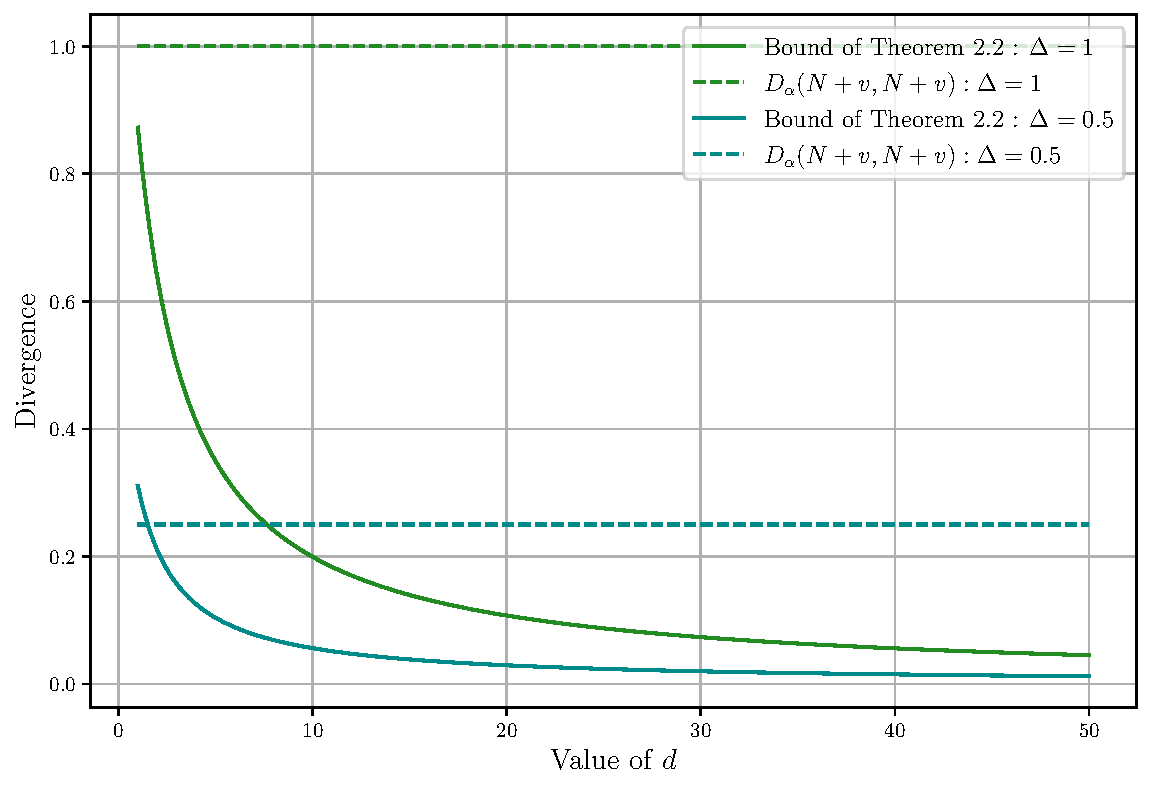
\includegraphics[width=0.5\linewidth]{generalAmplificationOneDim.pdf}
    \caption{Privacy bounds of Theorem~\ref{thm:upper-bound-renyi-one-dim} as a function of $d$ for multiple values of $\Delta$, $C = \sigma = 1$.}
    \label{fig:general-amplification-one-dim}
\end{figure}


\newpage


\section{Privacy amplification in multivariate linear regression}
In this section, we note $P_v$ the distribution of $(N+v)^\top(N+v)$, which is a non-central Wishart distribution $\mathcal{W}(n,d,\Omega_v)$ with non-centrality parameter $\Omega_v = v^\top v$:
\[P_v(y) = P_0(y) e^{-tr(\Omega_v)/2} {}_0F_1\left(\frac{d}{2}, \frac{1}{4}y^{1/2} \Omega_v y^{1/2} \right),\]
where $P_0$ is the central Wishart density $\mathcal{W}(k,d)$, and ${}_0F_1$ is the generalized hypergeometric function.

We state some properties of ${}_0F_1$:

\begin{proposition}[Properties of ${}_0F_1$~\citep{Muirhead2009}]
${}_0F_1$ has the following properties:
    \begin{itemize}
        \item Conjugation invariance: Let $U \sim O(k)$, then: \[{}_0F_1(a,Z) = {}_0F_1(a, U Z U^T).\]
        \item Dependence on eigenvalues: if $Z,Z'$ have the same eigenvalues with the same algebraic multiplicities, then: \[{}_0F_1(a,Z) = {}_0F_1(a, Z').\]
    \end{itemize}
\end{proposition}

\subsection{Proof of Theorem~\ref{prop:fisher-upper-bound-multi-dim}}
\label{app:prop-fisher-upper-bound-multi-dim}

\propFisherUpperBoundMultiDim*

\begin{proof}
    Let $\Sigma_v, \Sigma_w \in \mathbb{R}^{d \times k}$ be two rectangular diagonal matrices. Let $S_v,S_w \in O(k)$ and $U_v, U_w \in O(d)$ be orthogonal matrices. We note $v = U_v^\top\Sigma_vS_v, w = U_w^\top\Sigma_wS_w$. Let $\theta \in (0,1)$. Let $U \in O(d)$ be an orthogonal matrix. Define $f : \omega_1,\dots, \omega_{k + 1} \mapsto \sum_{i=1}^{k+1} \omega_i$. 

    Now, let $\Sigma_\theta \in \mathbb{R}^{n \times d}$ such that $\Sigma_0 = \Sigma_v$ and $\Sigma_1 = \Sigma_w$. Let $S_\theta \in O(k)$ such that $S_0 = I_k$ and $S_1 = S_w$, and $U_\theta \in O(d)$ such that $U_0 = U_v$ and $U_1 = U_w U$. For $i \in \{1,\dots,d\}$, we note $\mu(\theta) =\Sigma_\theta S_\theta$ and $v_\theta = U_\theta\mu(\theta)$ Since $\Sigma_\theta$ is rectangular diagonal, $\mu(\theta)$ has the form: $\mu(\theta) = \begin{pmatrix} M(t) \\ 0_{(d-k)\times k}
    \end{pmatrix}$. $\mu_i(\theta) \in \mathbb{R}^{k}$ is a column vector. Also, we note $V_\theta = N + v_\theta$.
    Then, by invariance of Gaussian matrices by orthogonal transformations: \[V_\theta^\top V_\theta = (N+U_\theta\mu(\theta))^\top (N + U_\theta \mu(\theta)) \overset{d}{=}(N+\mu(\theta))^\top (N+\mu(\theta))\]

We define $\omega_i = (N_i+\mu_i(\theta)^\top)^\top (N_i+\mu_i(\theta))+ \sum_{j=1}^{\lfloor d/k \rfloor-1} N^\top_{jk + i} N_{jk+i}$. Then, we have:
\begin{alignat*}{2}
    V_\theta^\top V_\theta &= \left(\sum_{i=1}^{k} \left((V_\theta^\top)_i (V_\theta)_i + \sum_{j=1}^{\lfloor d/k \rfloor-1} (V_\theta^\top)_{jk + i} (V_\theta)_{jk+i}\right)\right) + \sum_{i=k\lfloor d/k \rfloor}^{d} (V_\theta)^\top_i (V_\theta)_i \\
    &= \left(\sum_{i=1}^{k} \left((N_i+\mu_i(\theta)^\top)^\top (N_i+\mu_i(\theta)^\top)+ \sum_{j=1}^{\lfloor d/k \rfloor-1} N^\top_{jk + i} N_{jk+i}\right)\right) + \sum_{i=k\lfloor d/k \rfloor}^{d} N^\top_i N_i\\
    &= f\left(\omega_1,\dots,\omega_k, \sum_{i=k\lfloor d/k \rfloor}^{d} N^\top_i N_i\right)
\end{alignat*}

Then, by post-processing and independence of the packs:
\begin{align*}
    I(\theta) &= I(\theta,f(\mathcal{W}(k,\lfloor d/k \rfloor,\mu_1(\theta) \mu_1(\theta)^\top), \dots \mathcal{W}(k,\lfloor d/k \rfloor,\mu_k(\theta) \mu_k(\theta)^\top),\mathcal{W}(k,d-k\lfloor d/k \rfloor,0)))\\
    & \leq \sum_{i=1}^{k} I(\theta, \mathcal{W}(k,\lfloor d/k \rfloor,\mu_i(\theta)\mu_i(\theta)^\top))\\
\end{align*}
We note $m = \lfloor d/k \rfloor$. In the pack $ \mathcal{W}(k,m,\mu_i(\theta) \mu_i(\theta)^\top)$, we note $G \in \mathbb{R}^{m \times k}$ a Gaussian matrix and $X_i(\theta) = G + e_1\mu_i(\theta)^\top$. Then, $X_i(\theta)^\top X_i(\theta) \sim  \mathcal{W}(k,m,\mu_i(\theta) \mu_i(\theta)^\top)$.


Now, we compute a upper bound to the Fisher information $I(\theta, \mathcal{W}(k,m,\mu_i(\theta) \mu_i(\theta)^\top)$ of $ \mathcal{W}(k,m,\mu_i(\theta) \mu_i(\theta)^\top)$ for the parameter $\theta$.

The density writes:
\[p_t(y) = p_0(y)e^{-\tr(\mu_i(\theta)^\top \mu_i(\theta))/2} {}_0F_1\left( \frac{m}{2}, \frac{1}{4} y^{1/2} \mu_i(\theta) \mu_i(\theta)^\top y^{1/2}\right).\]
Since $\mu_i$ is a vector, the ${}_0F_1$ term reduces to the scalar ${}_0F_1$ function of its single non-zero eigenvalue:
\[{}_0F_1\left( \frac{m}{2}, \frac{1}{4} y^{1/2} \mu_i(\theta) \mu_i(\theta)^\top y^{1/2}\right) = {}_0F_1\left( \frac{m}{2}, \frac{1}{4} \mu_i(\theta)^\top y \mu_i(\theta) \right).\]
In fact, $y^{1/2} \mu_i(\theta) \mu_i(\theta)^\top y^{1/2}$ has $\mu_i(\theta)^\top y \mu_i(\theta)$ as only non-zero eigenvalue. 

We note, for $x > 0$, $F(d,x) = \log {}_0F_1(d,x)$. Also, we note $\mu_i(\theta) = \rho_i(\theta) u_i(\theta)$, where $\rho_i(\theta) > 0$ and $\|u_i(\theta)\| = 1$. This parametrization is interesting because $\langle u_i(\theta) ,\dot u_i(\theta) \rangle = 0$, so that $\langle \mu_i(\theta), \dot \mu_i(\theta)\rangle = \rho_i(\theta)\dot\rho_i(\theta)$.

Then, $\dot \mu_i(\theta) = \dot \rho_i(\theta) u_i(\theta) + \rho_i(\theta) \dot u_i(\theta)$, $\mu_i(\theta)^\top y \mu_i(\theta) = \rho_i(\theta)^2 q_\theta$ and $\mu_i(\theta)^\top y \mu_i(\theta) = \rho_i(\theta) (\dot\rho_i(\theta) u(t)^\top + \rho_i(\theta) \dot u(t))y U_\theta(t) = \rho_i(\theta)^2 r_\theta + \rho_i(\theta)\dot \rho_i(\theta) q_\theta$.

 We also write $q_\theta = u_i(\theta)^\top y u_i(\theta) = \|X_i(\theta) u_i(\theta)\|^2$ and $r_\theta = \dot u_i(\theta)^\top y u_i(\theta) = \langle X_i(\theta)u_i(\theta), X_i(\theta) \dot u_i(\theta)\rangle$. 
Then, the score function writes:

\begin{align*}
    \partial_\theta \log p_t (y) &= -\frac{1}{2}\partial_\theta \|\Omega_\theta\|_F^2 +\partial_\theta \log {}_0F_1\left( \frac{m}{2},  \frac{1}{4} \mu_i(\theta)^\top y \mu_i(\theta) \right) \\&= -\langle \mu_i(\theta),\dot \mu_i(\theta)\rangle + \frac{1}{2}F'\left( \frac{m}{2},  \frac{1}{4} \mu_i(\theta)^\top y \mu_i(\theta) \right) \dot \mu_i(\theta)^\top y \mu_i(\theta)\\
    &= -\langle \mu_i(\theta),\dot \mu_i(\theta)\rangle + \frac{1}{2}F'\left(\frac{m}{2}, \frac{\rho_i(\theta)^2}{4} q_\theta \right) (\rho_i(\theta)^2 r_\theta + \rho_i(\theta)\dot \rho_i(\theta) q_\theta),
\end{align*}

 Also, we relate the scalar ${}_0F_1$ function to modified Bessel functions of first kind:
\[{}_0F_1\left( \frac{m}{2}, x\right) = \Gamma(m/2)x^{1/2 - m/4} I_{m/2-1}(2\sqrt{x}).\]


Differentiating $\log {}_0F_1(m/2,x)$ and leveraging the relationship $2\sqrt{x}\frac{I_{m/2-1}'(2\sqrt{x})}{I_{m/2-1}(2\sqrt{x})} = \frac{m}{2}-1 + 2\sqrt{x}R_{m/2-1}(2\sqrt{x})$ from the proof of Proposition~\ref{prop:Fisher-upper-bound-one-dim}, we get:
\begin{align*}
    G(m/2,x)  &=  \frac{1-\frac{m}{2}}{2x} + \frac{1}{\sqrt{x}} \frac{I_{m/2-1}'(2\sqrt{x})}{I_{m/2-1}(2\sqrt{x)}} = \frac{1}{\sqrt{x}} R_{m/2-1}(2\sqrt{x}).
\end{align*}

Then, the score function writes:

\[\partial_\theta \log p_t(y) =  \dot \rho_i(\theta) \left(- \rho_i(\theta) +  \sqrt{q_\theta} R_{m/2-1}\left(\rho_i(\theta)\sqrt{q_\theta}\right) \right) + \frac{\rho_i(\theta) r_\theta }{\sqrt{q_\theta}}R_{m/2-1}\left(\rho_i(\theta)\sqrt{q_\theta}\right).\]

Now, we observe that $X_i(\theta) u_i(\theta)$ is a Gaussian vector. Then, $q_\theta = \|X_i(\theta) u_i(\theta)\|^2 = \|G u_i(\theta) + \rho_i(\theta) e_1\|^2$ follows a non-central chi-squared distribution $\chi_m^2(\rho_i(\theta)^2)$ with non-centrality $\rho_i(\theta)^2$ and degree of freedom $m$. Moreover, we observe that $X_tu_i(\theta)$ and $X_t \dot u_i(\theta)$ are independent. In fact, $\langle u_i(\theta), \dot u_i(\theta) \rangle = 0$. Also, $X_i(\theta) \dot u_i \sim \mathcal{N}(\rho_i(\theta) \langle u_i(\theta), \dot u_i(\theta)\rangle e_1, \|\dot u_i(\theta)\|^2 I_m) = \mathcal{N}(0,\|\dot u_i(\theta)\|^2 I_m)$. Then, we have:
\[r_\theta | \{ X_i(\theta) u_i(\theta) = z\} = \langle X_i(\theta)u_i(\theta), X_i(\theta) \dot u_i(\theta) \rangle | \{X_i(\theta) u_i(\theta) = z\} \sim \mathcal{N}(0, z^2\|\dot u_i(\theta)\|^2).\]

In particular, we have:
\[ \mathbb{E}[r_\theta | q_\theta] = 0, \;\; \mathbb{E}[r_\theta^2 | q_\theta ] = q_\theta\|\dot u_i(\theta)\|^2.\]

Also, we recall that $\|\dot \mu_i(\theta)\|^2 = \|\dot \rho_i(\theta) u_i(\theta) + \rho_i(\theta) \dot u_i(\theta)\|^2 = \dot \rho_i(\theta)^2 + \rho_i(\theta) \|\dot u_i(\theta)\|^2$.

We can now compute the Fisher information:
\begin{align*}
    &I(t, \mathcal{W}(k,\lfloor d/k \rfloor,\mu_i(\theta) \mu_i(\theta)^\top)\\&= \mathbb{E}\left[\left(\dot \rho_i(\theta) \left(- \rho_i(\theta) +  \sqrt{q_\theta} R_{m/2-1}\left(\rho_i(\theta)\sqrt{q_\theta}\right) \right) + \frac{\rho_i(\theta) r_\theta }{\sqrt{q_\theta}}R_{m/2-1}\left(\rho_i(\theta)\sqrt{q_\theta}\right)\right)^2 \right] \\
    &= \mathbb{E}\left[\mathbb{E}\left[\left(\dot \rho_i(\theta) \left(- \rho_i(\theta) +  \sqrt{q_\theta} R_{m/2-1}\left(\rho_i(\theta)\sqrt{q_\theta}\right) \right) + \frac{\rho_i(\theta) r_\theta }{\sqrt{q_\theta}}R_{m/2-1}\left(\rho_i(\theta)\sqrt{q_\theta}\right)\right)^2 \Bigg| q_\theta \right]\right] \\
    &= \mathbb{E}\left[\dot \rho_i(\theta)^2 \left(- \rho_i(\theta) +  \sqrt{q_\theta} R_{m/2-1}\left(\rho_i(\theta)\sqrt{q_\theta}\right) \right)^2   \right] \\
    &+2 \mathbb{E}\left[\left(\dot \rho_i(\theta) \left(- \rho_i(\theta) +  \sqrt{q_\theta} R_{m/2-1}\left(\rho_i(\theta)\sqrt{q_\theta}\right) \right) \frac{\rho_i(\theta) \mathbb{E}[r_\theta|q_\theta] }{\sqrt{q_\theta}}R_{m/2-1}\left(\rho_i(\theta)\sqrt{q_\theta}\right)\right)^2 \right] \\
    &+ \mathbb{E}\left[ \frac{\rho_i(\theta)^2\mathbb{E}[r_\theta^2|q_\theta]  }{q_\theta}R_{m/2-1}\left(\rho_i(\theta)\sqrt{q_\theta}\right)^2 \right]\\
    &= \dot \rho_i(\theta)^2 \mathbb{E}\left[ \left(- \rho_i(\theta) +  \sqrt{q_\theta} R_{m/2-1}\left(\rho_i(\theta)\sqrt{q_\theta}\right) \right)^2 \right] + \rho_i(\theta)^2\|\dot u_i(\theta)\|^2\mathbb{E}\left[R_{m/2-1}\left(\rho_i(\theta)\sqrt{q_\theta}\right)^2 \right]\\
\end{align*}
Now, we relate this expectation to the Fisher information of a non-central chi-squared distribution $\chi_m^2(\rho_i(\theta)^2)$ for the amplitude parameter $\rho_i(\theta)$. The density writes:
\[p_{\rho_i(\theta)}(x) = \frac{1}{2}e^{-(x + \rho_i(\theta)^2)/2} \left(\frac{x}{\rho_i(\theta)^2}\right)^{m/4-1/2} I_{m/2-1}\big(\rho_i(\theta)\sqrt{x}\big).\]
Then, the score function is: \begin{align*}
    \partial_{\rho_i(\theta)} \log p_{\rho_i(\theta)}(x) = - \rho_i(\theta) + \frac{1-m/2}{\rho_i(\theta)} + \sqrt{x}\frac{I_{m/2-1}'(\rho_i(\theta)\sqrt{x})}{I_{m/2-1}(\rho_i(\theta)\sqrt{x})} =  - \rho_i(\theta) + \sqrt{x} R_{m/2-1}(\rho_i(\theta) \sqrt{x}).
\end{align*}

Then, noting $Y \sim \chi_m^2(\rho_i(\theta)^2)$ and leveraging $\mathbb{E}_Y[\partial_{\rho_i(\theta)} \log p_{\rho_i(\theta)}(Y)] = 0$, the associated Fisher information $I(\rho_i(\theta))$ is equal to:
\begin{align*}
    I(\rho_i(\theta)) &= \mathbb{E}_Y\left[\left(- \rho_i(\theta) + \sqrt{Y} R_{m/2-1}\left(\rho_i(\theta) \sqrt{Y}\right)\right)^2\right]\\ &= \rho_i(\theta)^2 + \mathbb{E}_Y\left[\left(\sqrt{Y} R_{m/2-1}\left(\rho_i(\theta) \sqrt{Y}\right)\right)^2\right]- 2 \rho_i(\theta) \mathbb{E}_Y\left[\sqrt{Y} R_{m/2-1}\left(\rho_i(\theta) \sqrt{Y}\right)\right]\\
    &= \mathbb{E}_Y\left[Y R_{m/2-1}\left(\rho_i(\theta) \sqrt{Y}\right)^2\right] - \rho_i(\theta)^2.
\end{align*}

Then, the Fisher information writes:
\[I(\theta, \mathcal{W}(k,\lfloor d/k \rfloor,\mu_i(\theta) \mu_i(\theta)^\top) = \dot \rho_i(\theta)^2 I(\rho_i(\theta)) + \rho_i(\theta)^2 \|\dot u_i(\theta)\|^2 \mathbb{E}\left[R_{m/2-1}\left(\rho_i(\theta)\sqrt{q_\theta}\right)^2 \right].\]
Now, we connect $I(\rho_i(\theta))$ to $\mathbb{E}\left[R_{m/2-1}(2\sqrt{q_\theta})^2 \right] = \mathbb{E}_Y\left[R_{m/2-1}\left(2\sqrt{Y}\right)^2 \right]$. Since $R_{m/2-1}$ is increasing, we can apply the Chebyshev integral inequality:

\begin{align*}
    \mathbb{E}\left[R_{m/2-1}\left(2\sqrt{q_\theta}\right)^2 \right] \leq \frac{\mathbb{E}_Y\left[YR_{m/2-1}\left(2 \rho_i(\theta) \sqrt{Y}\right)^2 \right]}{\mathbb{E}_Y\left[Y \right]} = \frac{I(\rho_i(\theta)) + \rho_i(\theta)^2}{m + \rho_i(\theta)^2} &\leq \frac{\rho_i(\theta)^2 (2\rho_i(\theta)^2 + m - 1) }{(2\rho_i(\theta)^2 + m - 3)(\rho_i(\theta)^2 + m)}\\
    &\leq \frac{2\rho_i(\theta)^2 }{2\rho_i(\theta)^2 + m - 3},
\end{align*}
leveraging the Fisher information upper bound for non-central chi-squared distributions of~\ref{prop:Fisher-upper-bound} $I(v_i) \leq \frac{2 v_i^2}{2 v_i^2 + m - 3}$.

Therefore,

\begin{align*}
    I(\theta, \mathcal{W}(k,\lfloor d/k \rfloor,U_\theta^\top \Lambda^{\top}_i \Lambda_i U_\theta)) &\leq  \dot \rho_i(\theta)^2 I(\rho_i(\theta)) + \rho_i(\theta)^2 \|\dot u_i(\theta)\|^2  \frac{2\rho_i(\theta)^2 }{2\rho_i(\theta)^2 + m - 3}\\
    &\leq (\dot \rho_i(\theta)^2 + \rho_i(\theta)^2 \|\dot u_i(\theta)\|^2 ) \frac{2\rho_i(\theta)^2 }{2\rho_i(\theta)^2 + m - 3}\\
    &\leq \|\dot \mu_i(\theta)\|^2 \frac{2\rho_i(\theta)^2 }{2\rho_i(\theta)^2 + m - 3}.
\end{align*}


From there, we upper bound the total Fisher information by leveraging the concavity of $x \mapsto \frac{x}{x+c}$ on $\mathbb{R}^+$ for the inputs $\|\dot \mu_i(\theta)\|^2$:
\begin{align}
    I(\theta) &\leq \sum_{i=1}^k \|\dot \mu_i(\theta)\|^2 \frac{2\rho_i(\theta)^2 }{2\rho_i(\theta)^2 + m - 3}\\
    &\leq \|\dot \mu(\theta)\|_F^2 \frac{2\sum_{i=1}^k \rho_i(\theta)^2 \dot \mu_i(\theta)^2 / \|\dot \mu(\theta)\|_F^2}{\sum_{i=1}^k  \rho_i(\theta)^2 \dot \mu_i(\theta)^2 / \|\dot \mu(\theta)\|_F^2 + m - 3}\\
    &\leq \|\dot \mu(\theta)\|_F^2 \frac{\rho(\theta)^2}{\rho(\theta)^2 + m - 3}.
\end{align}


Now, taking $\mu(\theta) = (1-\theta) v + \theta Uw$, we get $\dot \mu(\theta) = Uw-v$, and $\rho(\theta) = \|(1-\theta) v + \theta Uw\|_F$, giving the desired result.

\end{proof}

\newpage
\subsection{Upper bounding the divergence in the general case}
\label{app:prop-renyi-upper-bound-multi-dim}

% Leveraging Proposition~\ref{app:prop-fisher-upper-bound-multi-dim} and Proposition~\ref{prop:Fisher-upper-bound}, we get the following upper bound to the Rényi divergence $D_\alpha(V^\top V, W^\top W)$:
% \begin{theorem}[Privacy in the $n_{\mathrm{syn}} \to + \infty$ regime]
%     Assume without loss of generality that $\| w\|_1 \leq \|v\|_1$ and note: \[I(k,d,v) = \frac{\|v\|_F^2 (\|v\|_F^2 + 2k\lfloor d/k \rfloor)}{2k\lfloor d/k \rfloor^2 + 2 \|v\|_F^2 (\|v\|_F^2 + 2k\lfloor d/k \rfloor)}.\]
%     Then, we have:
%     \begin{align*}
%         D_\alpha(V^\top V,W^\top W) 
%         \leq \frac{1}{\alpha-1}\log\left(1+2\alpha \sigma^2 I(k,d,v)^{1/2}\frac{e^{(\alpha-1) (2\alpha-1) \frac{\Delta^2}{2\sigma^2}} -1}{(\alpha-1)(2\alpha-1)\Delta}\right),
%     \end{align*}
% \end{theorem}

\subsection{Proof of Proposition~\ref{prop:Fisher-upper-bound-one-dim}}
\label{app:improvement-fisher-multiple}
In this section, we outline another upper bound for the Fisher information of non-central chi-squared distributions. This upper bound is worse than the upper bound of Proposition~\ref{prop:Fisher-upper-bound-one-dim}, but we think that the proof technique is worth of noting. In fact, the proof technique is different and relies on a Poincaré inequality step. We highlight this proof technique because we think that a similar proof could be developed for non-central Wishart distributions, giving a potential better Fisher information than the one we obtain in this paper. To develop the same upper bounds for non-central Wishart distribution, we need a control on the spectrum of the Hessian of ${}_0F_1$, which appears when performing the Poincaré inequality step. We believe that this could be done through the integral representation of ${}_0F_1$ (Proposition~\ref{prop:integral-representation}).
\begin{restatable}{proposition}{propFisherUpperBoundOneDimWorse}\normalfont(Fisher information of non-central $\chi^2$).
\label{prop:Fisher-upper-bound-one-dim-worse}
For all $\theta> 0$ and  $p_\theta \in P$, and :
    \[I(\theta) \leq \frac{2\theta^2(\theta^2 + 2d)}{2d^2 +  \theta^2(\theta^2 + 2d)}.\]
\end{restatable}

\begin{proof}
    We note $\lambda = \theta^2/2$.
    Let $\pi_\lambda(i) = e^{-\lambda} \lambda^i /i!$ be the Poisson probability mass function and $f_i = \frac{x^{i/2-1} e^{-x/2}}{2^{i/2}\Gamma(i/2)}$ the chi-squared density with $i$ degrees of freedom.
    We write non-central chi squared random variables as Poisson-weighted mixture of central chi squared random variables: \[p_\theta = \sum_{i=0}^{+\infty} \pi_{\theta^2/2}(i)f_{d+2i}.\]
    Then, using $\partial_\theta \pi_{\theta^2/2}(i)= (- \theta  + \frac{2 i}{\theta} )  \pi_{\theta^2/2}(i)$
    \[\partial_\theta p_\theta = \sum_{i=0}^{+\infty} \left(- \theta  + \frac{2 i}{\theta} \right)\pi_{\theta^2/2}(i)f_{d+2i},\]
    We note $K \sim Poisson(\theta^2/2)$, and $Y | K=i\sim Gamma(d/2 + i, 2)$. Then,\[s_\theta^2 = \left(\frac{\partial_\theta p_\theta}{p_\theta}\right)^2 =\mathbb{E}\left[ -\theta + \frac{2K}{\theta} \bigg | Y \right]^2 = \frac{4}{\theta^2}\left(\mathbb{E}[K | Y] - \frac{\theta^2}{2}\right)^2,\]
    and finally
    \[I(\theta) = \mathbb{E}_\theta\left[s_\theta^2\right] = \frac{4}{\theta^2}\Var\left(\mathbb{E}[K|Y]\right).\]
    We want to compute a upper bound to $\Var(\mathbb{E}[K|Y])$. 

    The variable $K|Y = y$ follows the Bessel distribution~\citep{Yuan2000} with parameters $Bessel(\sqrt{\lambda y},d/2 -1)$. Then,

\[E[K|Y] = \frac{1}{2} \sqrt{\lambda Y} \frac{I_{d/2}(\sqrt{\lambda Y})}{I_{d/2-1}(\sqrt{\lambda Y})},\]
where $I_{d/2}$ is the modified Bessel function of index $d/2$.

Let $g : Z \mapsto \sum_{i=1}^d (z_i + v_i)^2 = \|Z+V\|_F^2$, with $Z \sim \mathcal{N}(0, I_d)$, $f_\nu : y \mapsto \frac{1}{2}yR_\nu(y)$, and $x = \sqrt{\lambda y}$. Then, \[\frac{df_\nu}{dy}(x) = \frac{\lambda}{4x}\left(R_\nu(x) + x R_\nu'(x)\right).\]

Using the identity:
\[R'_\nu(x)=1 - \frac{2(\nu-1)}{x}R_\nu(x) - R_\nu(x)^2,\]
we get:
\[\frac{df_\nu}{dy}(x) = \frac{\lambda}{4}\left(1- R_\nu(x)^2 - \frac{2(\nu-1)}{x}R_\nu(x)\right).\]

A known sharp inequality for Bessel quotients is, for $\nu > 1/2$~\citep{ruiz2016}:

\[\frac{x}{\nu + \sqrt{\nu^2 + x^2}} \leq \frac{I_{\nu}(x)}{I_{\nu-1}(x)}  \leq \frac{x}{\nu-1/2 + \sqrt{(\nu-1/2)^2 + x^2}}.\]

Then,

\begin{align*}
    \frac{df_\nu}{dy}(x) &\leq \frac{\lambda}{4}\left(1- \left(\frac{x}{\nu + \sqrt{\nu^2 + x^2}}\right)^2 - \frac{2(\nu-1)}{x}\frac{x}{\nu + \sqrt{\nu^2 + x^2}} \right)\\
    &\leq \frac{\lambda}{4 }\left(\frac{2\nu}{\nu + \sqrt{\nu^2 + x^2}} -\frac{2(\nu-1) }{\nu + \sqrt{\nu^2 + x^2}} \right)\\
    &\leq \frac{\lambda}{2}\frac{1}{\nu + \sqrt{\nu^2 + x^2}}.
\end{align*}



The Poincaré inequality gives:

\begin{align*}
    \Var\left( \frac{1}{2} \sqrt{\lambda Y} \frac{I_{d/2}(\sqrt{\lambda Y})}{I_{d/2-1}(\sqrt{\lambda Y})} \right)  =& \; \Var\left(f_{(d-1)/2} \circ g(Z) \right) \\ \leq&\; \mathbb{E}\left[\|\nabla (f_{(d-1)/2} \circ g (Z)) \|_F^2\right] \\ 
    =&\; \mathbb{E}\left[4 (f'_{(d-1)/2} \circ g (Z))^2 \|Z+v\|_F^2\right]\\
    =&\; \mathbb{E}\left[ 4\left(\frac{\lambda}{2}\frac{1}{\nu + \sqrt{\nu^2 + \lambda Y}}\right)^2 Y\right]\\
    =& \;\lambda^2\mathbb{E}\left[ \frac{Y}{2\nu^2 +  \lambda Y} \right].
\end{align*}

Then, taking $\nu = d/2$ and by concavity of $y \mapsto \frac{y}{2\nu^2 + \lambda y}$, Jensen inequality gives:
\[I(\lambda) \leq 2\lambda\frac{\mathbb{E}\left[Y\right]}{2(d/2)^2 +  \lambda \mathbb{E}\left[Y\right]} =  \frac{4\lambda(\lambda + d)}{d^2 +  2\lambda(\lambda + d)}\leq \frac{2\theta^2(\theta^2 + 2d)}{2d^2 +  \theta^2(\theta^2 + 2d)}.\]

\end{proof}



\newpage





%\begin{proof}
%    The proof is the same as the proof of Theorem~\ref{thm:upper-bound-renyi-one-dim}, but in this case, we have to prove that the Rényi divergence is differentiable in the case $k > 1$. Leveraging the density of non central Wishart distribution, the proof is essentially the same as the proof of Lemma~\ref{lem:differentiability-one-dim}, but in this case, we have to prove domination of gradients of hypergeometric functions. An integral representation
%\end{proof}

\section{Numerical estimation of the divergence}
\label{app:experiments}
In this section, we restate the discussion of Section~\ref{sec:experiments} and add details for completeness.

We perform a series of experiments designed to illustrate our theoretical results. While sampling from $ZV$ is straightforward, its density is analytically intractable. Therefore, we rely on variational inference methods to estimate the Rényi divergence $D_\alpha(ZV,ZW)$. Specifically, we numerically estimate the Rényi divergence induced by releasing $ZV$ using the \emph{Convex-Conjugate Rényi Variational Formula}, introduced~\cite{birrell2023} (Theorem 2.1).

\begin{theorem}[Convex-Conjugate Rényi Variational Formula (Theorem 2.1 from~\citep{birrell2023})]
Let $(\Omega, \mathcal{M})$ be a measurable space, $P, Q \in \mathcal{P}(\Omega)$, and $\alpha \in (0,1) \cup (1,\infty)$. Then,
\[D_\alpha(P,Q) =\alpha \sup_{g \in \mathcal{M}_b(\Omega); g < 0} \left\{ \int gdQ + \frac{1}{\alpha - 1} \log \int |g|^{(\alpha-1)/\alpha} dP \right\} + \log \alpha + 1,\]
where $\mathcal{M}_b(\Omega)$ is the space of bounded functions on $\Omega$.
\end{theorem}

Among existing variational methods to estimate the Rényi divergence, this formula has the specificity of being well-behaved when $\alpha > 1$~\citep{birrell2023}, which aligns with our setting. In order to estimate the Rényi divergence between two distributions $P,Q$, we proceed as follows. We initialize a two layers neural network $f(w_0,\cdot)$ with negative poly-softplus activation~\citep{birrell2023} and train it to maximize:
\[\sup_{w} \left\{ \int f(w)dQ + \frac{1}{\alpha - 1} \log \int |f(w)|^{(\alpha-1)/\alpha} dP \right\}\]
Optimization is performed via minibatch stochastic gradient ascent. At each iteration, we sample $X = (X_1,\dots, X_l) \sim P^{\otimes l}$, $Y = (Y_1,\dots,Y_l) \sim Q^{\otimes l}$ for some batch size $l > 0$ and update the network parameters using the empirical objective:
\[F(w,X,Y) =\frac{1}{l}\sum_{i=1}^lf(w,Y_i)+  \frac{1}{
\alpha - 1}\log\left( -\frac{1}{l}\sum_{i=1}^l f(w,X_i)^{(\alpha-1)/\alpha}\right).\]
Each estimation is performed $10$ times and the results are averaged. For reproducibility, here are some experimental details:
\begin{itemize}
    \item Number of training steps: $2\cdot 10^4$.
    \item Batch size: $512$.
    \item Learning rate: $10^{-3}$.
    \item Hidden dimension: $64$.
    \item Final activation: Poly-softplus~\citep{birrell2023}.
    \item Optimizer: Adam~\citep{Kingma2014}.
    \item Validation score is computed every $100$ steps with a resampled validation set of size $5 \times 10^4$.
    \item Early stopping criterion: No validation score improvement for $10$ validation steps.
    \item Once trained, the divergence estimation is made on a sample of size $5 \times 10^4$.
\end{itemize}
At each step, data is resampled from the distributions of $ZV$ and $ZW$.

\subsection{Proofs of Proposition~\ref{prop:privacy-gap} and Corrolary~\ref{corr:privacy-gap-scaling}}
In this section, we derive a lower bound on $D_\alpha(ZV,ZW) - D_\alpha(V^\top V, W^\top W)$ in the case $k=1$. In this setting, we leverage the fact that $D_\alpha(ZV,ZW) = D_\alpha(V^\top Z^\top Z V, W^\top Z^\top Z W) = D_\alpha(\|ZV\|^2,\|ZW\|^2)$.
Here, $ZV \in \mathbb{R}^{n_{\text{syn}}}$. Also, $V^\top V = \|V\|^2$ follows a non-central chi-squared distribution $\chi_d^2(\|v\|^2)$ with degree of freedom $d$ and non-centrality parameter $\|v\|^2$. To simplify notations, we note $n=n_{\text{syn}}$ and: $S_v = \frac{1}{n_{\text{syn}}}\|ZV\|^2$ and $Y_v = \|V\|^2$. We note the measures: $\mu_n = P\left(\frac{1}{n_{\text{syn}}}\|ZV\|^2\right), \nu_n = P\left(\frac{1}{n_{\text{syn}}}\|ZW\|^2\right), \mu = \|V\|^2$ and $ \nu = \|W\|^2$. Also, for $s > 0$, we note $r(x) = \frac{d\mu}{d\nu}(s)$.

\begin{lemma}
    Assume that $k=1$. Let $\alpha > 1$. For two distributions $P, Q$, we note $H_\alpha(P,Q) = \exp((\alpha-1)D_\alpha(P,Q))$. Let $X_n \sim \frac{1}{n}\chi_{n}^2$ follow a (rescaled) chi-squared distribution with degree of freedom $n$. Then,
    \[H_\alpha(\mu, \nu) - H_\alpha(\mu_n, \nu_n) = \mathbb{E}_{S_w\sim \nu_n}\left[\mathbb{E}_{Y_w \sim \nu}[r(Y_w)^\alpha | Y_wX_n = S_w] - \mathbb{E}_{Y_w \sim \nu}\left[r(Y_w) \big| Y_wX_n = S_w \right]^\alpha\right].\]
\end{lemma}

\begin{proof}
    First, we notice that  $ZV | V \sim \mathcal{N}(0,\|V\|^2 I_{n})$. Let $X_n \sim \frac{1}{n}\chi_{n}^2$. Then, $S_v | Y_v = Y_v X_n$. $\mu_n$ and $\nu_n$ can be seen as the output of the same Markov kernel $K : y \mapsto yX_n$ for the measures $\mu$ and $\nu$. Thus, the density ratio $\frac{d\mu_{n}}{d\nu_{n}}(s)$ writes:
    \[\frac{d\mu_{n}}{d\nu_{n}}(s) = \mathbb{E}_{Y_w \sim\nu}\left[\frac{d\mu}{d\nu}(Y_w) \big| Y_wX_n = s \right] = \mathbb{E}_{Y_w \sim \nu}\left[r(Y_w) \big| Y_wX_n = s \right]\]
    Now, by definition,
    \[H_\alpha(S_v,S_w) = \mathbb{E}_{S_w \sim \nu_n}\left[\mathbb{E}_{Y_w \sim \nu}\left[r(Y_w) \big| Y_wX_n = S_w \right]^\alpha\right]\]
    
    Also by tower property, \[H_\alpha(Y_v,Y_w) = \mathbb{E}_{Y_w \sim \nu}\left[r(Y_w)^\alpha\right] = \mathbb{E}_{S_w \sim \nu_n}\left[\mathbb{E}_{Y_w \sim \nu}\left[r(Y_w)^\alpha \big| Y_wX_n = S_w \right]\right],\]
    giving the desired result.
    \end{proof}

    Now, we upper bound the quantity $H_\alpha(\mu, \nu) - H_\alpha(\mu_n, \nu_n)$. Our strategy relies on showing that, for large values of $n$, the ratio $r(Y_w)$ is concentrated around $\mathbb{E}[r(Y_w) | Y_w X_n = S_w]$ with high probability.

    \begin{lemma}
    \label{lem:divergence-decomposition-moments}
    Let $\alpha \geq 2$. We note $M(S_w) = \mathbb{E}[r(Y_w) | Y_w X_n = S_w]$. Then,
    
        \[H_\alpha(\mu, \nu) - H_\alpha(\mu_n, \nu_n) \leq \alpha(\alpha-1) 2^{\alpha-3}e^{(\alpha-1)(\alpha-2)\Delta^2/2} \|r(Y_w)-M(S_w)\|_\alpha^2.\]
    \end{lemma}
    
    \begin{proof}
    We have, by definition:
    \[\mathbb{E}[r(Y_w) - M(S_w)|Y_w X_n = S_w] = \mathbb{E}[r(Y_w) - M(S_w)|S_w]  =  0.\]
    Then, $\mathbb{E}[\alpha M^{\alpha-1}(S_w)(r(Y_w)-M(S_w))|S_w] = 0$. Let $\phi_\alpha: x \mapsto x^\alpha$ Then, leveraging $\alpha \geq 2$ and by the mean value theorem in the expectation in the interval $(\min(M(S_w),r(Y_w)),\max(M(S_w),r(Y_w))$, and $\max(M(S_w),r(Y_w)) \leq M(S_w) + r(Y_w)$:
    \begin{align*}
         H_\alpha(\mu, \nu) - H_\alpha(\mu_n, \nu_n) &= \mathbb{E}\left[\mathbb{E}[r(Y_w)^\alpha |S_w] -M(S_w)^\alpha\right]\\
        &= \mathbb{E}\left[\mathbb{E}[r^\alpha(Y_w) - M(S_w)^\alpha - \alpha M^{\alpha-1}(S_w)(r(Y_w)-M(S_w))|S_w]\right]\\
        &= \mathbb{E}\left[\mathbb{E}[\phi(r(Y_w)) - \phi(M(S_w)) -  (r(Y_w)-M(S_w)) \phi'(M(S_w))|S_w]\right]\\
        &=\frac{1}{2} \mathbb{E}\left[\mathbb{E}[\phi''(Z) (M(S_w)-r(Y_w))^2|S_w]\right], \;\;\;\; Z \in (\min(M(S_w),r(Y_w)),\max(M(S_w),r(Y_w))\\
        &\leq \frac{\alpha(\alpha-1)}{2} \mathbb{E}\left[\mathbb{E}[(M(S_w)+r(Y_w))^{\alpha-2} (M(S_w)-r(Y_w))^2|S_w]\right]\\
        &\leq \frac{\alpha(\alpha-1)}{2} \|r(Y_w)+M(S_w)\|_\alpha^{\alpha-2} \|r(Y_w)-M(S_w)\|_\alpha^2,
    \end{align*}
    where the last step is the Hölder inequality with exponents $\frac{\alpha}{\alpha-2}$ and $\frac{\alpha}{2}$.
    Now, by tower property and the Jensen inequality,
    \[\|M(S_w)\|_\alpha^\alpha  = \mathbb{E}[M(S_w)^\alpha] = \mathbb{E} [\mathbb{E}[r(Y_w)|S_w]^\alpha] \leq \mathbb{E} [\mathbb{E}[r(Y_w)^\alpha|S_w]] = \|r(Y_w)\|_\alpha^\alpha.\]
    Then, triangle inequality implies: 
    \[\|r(Y_w) + M(S_w)\|_\alpha \leq \|r(Y_w)\|_\alpha + \|M(S_w)\|_\alpha \leq 2 \|r(Y_w)\|_\alpha.\]
    Therefore,

    \[H_\alpha(\mu, \nu) - H_\alpha(\mu_n, \nu_n) \leq \alpha(\alpha-1) 2^{\alpha-3}\|r(Y_w)\|_\alpha^{\alpha-2} \|r(Y_w)-M(S_w)\|_\alpha^2.\]

    Also, we can relate $\|r(Y_w)\|_\alpha$ to $D_\alpha(V,W)$ by a post-processing argument: \[\|r(Y_w)\|_\alpha^\alpha = \mathbb{E}\left[r(Y_w)^\alpha\right] = e^{(\alpha-1)D_\alpha(\|V\|^2,\|W\|^2)} \leq e^{(\alpha-1)D_\alpha(V,W)} = e^{\alpha(\alpha-1)\Delta^2/2} .\]

    Then, we obtain: 
    \[H_\alpha(\mu, \nu) - H_\alpha(\mu_n, \nu_n) \leq \frac{\alpha(\alpha-1)}{2} 2^{\alpha-2}e^{(\alpha-1)(\alpha-2)\Delta^2/2} \|r(Y_w)-M(S_w)\|_\alpha^2.\]
    \end{proof}
    Now, we upper bound $\|r(Y_w)-M(S_w)\|_\alpha^2$ by a concentration argument:
    \begin{proposition}
    Let $\alpha \geq 2$. Then, there exists $C > 0$ such that $d > C$ implies:
        \[H_\alpha(\mu, \nu) - H_\alpha(\mu_n, \nu_n) = O(1/n),\]
        where the rate does not depend on $d$.
    \end{proposition}

    \begin{proof}
    First, for any measurable function $g$, $\|r(Y_w) - M(S_w)\|_\alpha \leq 2\|r(Y_w) - g(S_w)\|_\alpha$.
    In fact, $r(Y_w) - M(S_w) = r(Y_w) - g(S_w) - \mathbb{E}[r(Y_w) - g(S_w) | S_w]$ and the conditional expectation is a contraction of $L^\alpha(\mathbb{R)}$.
    
    Let $A = \{X_n \in (1/2, 2)\}$. Then, choosing $g(S_w) = r(S_w) \mathbbm{1}_A$, we have:
    \begin{align*}
        \|r(Y_w)-g(S_w)\|_\alpha^\alpha = \mathbb{E}[|r(Y_w) - r(S_w) \mathbbm{1}_A|^\alpha] = \mathbb{E}[|r(Y_w) - r(S_w)|^\alpha \mathbbm{1}_A] + \mathbb{E}[|r(Y_w)|^\alpha \mathbbm{1}_{A^C}].
    \end{align*}
        Therefore, we can decompose $\mathbb{E}[(r(Y_w) - M(S_w))^\alpha]$ into two terms:
    \[\mathbb{E}[(r(Y_w) - M(S_w))^\alpha] \leq  2^\alpha (\mathbb{E}[|r(Y_w) - r(S_w)|^\alpha \mathbbm{1}_{A}] + \mathbb{E}[|r(Y_w)|^\alpha\mathbbm{1}_{A^C}]).\]
    We upper bound both terms.
    First, we upper bound $P(A^C)$ by concentration. $X_n \sim \frac{1}{n}\chi_n^2$. The moment-generating function of $X_n$ is finite for $t \in (-\infty, n/2)$ and writes $M_{X_n}(t) = \left(1- \frac{2t}{n}\right)^{-n/2}$. Let $t\in (0,n/2)$. Then, the Chernoff inequality gives:
    \[P(X_n \geq 2) \leq M_{X_n}(t) e^{-2t}  =\exp\left(-2t - \frac{n}{2} \log(1-2t/n) \right).\]

    
    We find the lower bound of this inequality at $t^* =  n(1-\frac{1}{x})/2$.
    
    $P(X_n \geq 2) \leq e^{-\frac{n}{2}(1- \log 2)}$.
    Now, let $t < 0$. Since $x \mapsto e^{tx}$ is decreasing:
    \[P(X_n \leq 1/2) = P(e^{Xt} \geq e^{t/2})  \leq M_{X_n}(t) e^{-t/2} = \exp\left(-t/2 - \frac{n}{2} \log(1-2t/n) \right).\]
    We find the lower bound of this inequality at $t^* = -n/2$. Then, $P(X_n \leq 1/2) \leq e^{-\frac{n}{2}(\log 2 - 1/2)}$
    Also, $\log 2 - 1/2 \approx 0.19 \leq 1 - \log 2 \approx 0.31$.
    Therefore, $P(A^C) \leq 2 e^{-cn}$, with $c = \frac{1}{2}(\log 2 - 1/2)$.
    
    Let $p,q > 0$ such that $1/p + 1/q = 1$.
    \begin{align*}
        \mathbb{E}[(r(Y_w) - M(S_w))^\alpha\mathbbm{1}_{A^C}] &\leq P(A^C)^{1/p} \mathbb{E}[(r(Y_w) - M(S_w))^{\alpha q}]^{1/q} \\
        &\leq  2^{1/p}e^{-cn/p} \mathbb{E}[(r(Y_w) - M(S_w))^{\alpha q}]^{1/q}\\
    \end{align*}
    Also, leveraging Lemma~\ref{lem:divergence-decomposition-moments}, $\mathbb{E}[r(Y_w)^{\alpha q}] \leq e^{(\alpha q -1) \Delta^2/2}$.
    
    Therefore, taking $p=q=2$,
    \[ \mathbb{E}[(r(Y_w) - r(S_w))^\alpha\mathbbm{1}_{A^C}] \leq 2^{1/2}\exp(\alpha(2\alpha - 1) \Delta^2/2-cn/2).\]

    Now, we upper bound the quantity $\mathbb{E}[|1-X_n|^\alpha]$. $nX_n-n$ is a sub-Gamma random variable, since $n X_n - n \sim \Gamma(2n,2)$. From Theorem 2.3. of~\citet{Boucheron2013}, for even $\alpha > 1$, $\mathbb{E}[|n X_n - n|^\alpha] \leq (\alpha/2)! (16n)^{\alpha/2} + \alpha!8^\alpha \lesssim C_\alpha n^{\alpha/2}$.
    Dividing by $n^\alpha$, there exists $C_\alpha > 0$ such that $\mathbb{E}[|1-X_n|^\alpha] \leq C_\alpha n^{-\alpha/2}$. For other values of $\alpha$, we use the monotonicity of the $L_p$ norm to obtain the upper bound.
    
    
    Also, noticing $(r(Y_w) - r(Y_wX_n))^\alpha \mathbbm{1}_{A} \leq |Y_w - Y_wX_n|^\alpha\sup_{t \in (Y_w/2, 2Y_w)} r'(t)^\alpha = Y_w^\alpha|1 - X_n|^\alpha\sup_{x \in (1/2, 2)} r'(Y_w x)^\alpha$, we get:
    \begin{align*}
        \mathbb{E}[(r(Y_w) - r(S_w))^\alpha\mathbbm{1}_{A}]
     &\leq \mathbb{E}[Y_w^\alpha |1-X_n|^\alpha \sup_{x \in (1/2,2)} r'(Y_wx)^\alpha]\\
        &\leq\mathbb{E}[|1-X_n|^\alpha] \mathbb{E}[Y_w^\alpha  \sup_{x \in (1/\beta,\beta)} r'(Y_w x)^\alpha]\\
        &\leq C_\alpha n^{-\alpha/2}\mathbb{E}[Y_w^\alpha \sup_{x \in (1/2,2)} r'(Y_w x)^\alpha]
    \end{align*}

    Now, we evaluate $\mathbb{E}[Y_w^\alpha \sup_{x \in (1/\beta,\beta)} r'(Y_w x)^\alpha]$. We note $\lambda_v = \|v\|, \lambda_w = \|w\|$. Let $y > 0$. The density of $Y_w$ writes:

    \begin{align*}
        p_{\lambda_v}(y) = p_0(y) e^{- \lambda_v^2/2} \lambda_v^{1-d/2}  I_{d/2-1}\big(\lambda_v\sqrt{y}\big).
    \end{align*}

    Then, we write the ratio $r(y)$:
    \begin{align*}
        r(y) = e^{(\lambda_w^2-\lambda_v^2)/2} \left(\frac{\lambda_v}{\lambda_w}\right)^{1-d/2}\frac{I_{d/2-1}\big(\lambda_v\sqrt{y}\big)}{I_{d/2-1}\big(\lambda_w\sqrt{y}\big)}.
    \end{align*}
    We recall the following relationship:
    \[\lambda_v \sqrt{y}R_{d/2-1}(\lambda_v \sqrt{y}) + d/2 - 1= \lambda_v \sqrt{y} \frac{I_{d/2-1}'(\lambda_v \sqrt{y})}{I_{d/2-1}(\lambda_v \sqrt{y})}.\]

    Then, we compute a upper bound to $\frac{dr}{dy}(y)$.
    \begin{align*}
        \frac{dr}{dy}(y) &= \partial_y \log I_{d/2-1}(\lambda_v\sqrt{y})- \partial_y \log I_{d/2-1}(\lambda_w\sqrt{y})\\
        &= \frac{1}{2\sqrt{y}}\left(\lambda_v\frac{I_{d/2-1}'(\lambda_v\sqrt{y})}{I_{d/2-1}(\lambda_v\sqrt{y})} - \lambda_w\frac{I_{d/2-1}'(\lambda_w \sqrt{y})}{I_{d/2-1}(\lambda_w \sqrt{y})}\right)\\
        &= \frac{1}{2\sqrt{y}}\left(\lambda_vR_{d/2-1}(\lambda_v \sqrt{y}) - \lambda_wR_{d/2-1}(\lambda_w \sqrt{y})\right)\\
        &\leq \frac{1}{2\sqrt{y}}\left(\lambda_vR_{d/2-1}(\lambda_v \sqrt{y}) + \lambda_wR_{d/2-1}(\lambda_w \sqrt{y})\right)\\
        &\leq \frac{\lambda_v^2+ \lambda_w^2}{2d},
    \end{align*}
    where the Bessel quotient upper bound is obtained leveraging the following inequality:
    \[ 0 \leq R_{\nu}(y) =\frac{I_{\nu+1}(y)}{I
    _{\nu}(y)} \leq \frac{y}{2(\nu+1)}.\]


    Therefore, noting $B = (\lambda_v^2 + \lambda_w^2)/2$, $|r'(y)| = r(y) |\partial_y \log r(y) | \leq \frac{B}{d} r(y)$. Then, by Gronwall's inequality, for any $x \in (1/2,2)$, 
    \[r(yx) \leq r(y) e^{B y (x-1)/d}.\]
    Therefore, $\sup_{x \in (1/2,2)} |r'(Y_w x)| \leq \frac{B}{d} \sup_{x \in (1/2,2)} |r(Y_w x)| \leq \frac{B}{d} r(Y_w) e^{2yB/d}$.
    
    Then, we apply the generalized Hölder inequality:
    \begin{align*}
        \mathbb{E}[Y_w^\alpha \sup_{x \in (1/\beta,\beta)} r'(Y_wx)^\alpha] &\leq \frac{B^\alpha}{d^\alpha}  \mathbb{E}[Y_w^\alpha  r(Y_w)^\alpha e^{2\alpha Y_wC/d}]\\
        &\leq \frac{B^\alpha}{d^\alpha}  \mathbb{E}[Y_w^{3\alpha}]^{1/3} \mathbb{E}[e^{6\alpha Y_w B/d}]^{1/3} \mathbb{E}[r(Y_w)^{3\alpha}]^{1/3}\\
        &\leq \frac{B^\alpha}{d^\alpha}\mathbb{E}[Y_w^{3\alpha}]^{1/3} \mathbb{E}[e^{6\alpha Y_w B/d}]^{1/3} e^{(3\alpha-1)D_{2\alpha}(V,W)/3}\\
        &\leq \frac{B^\alpha}{d^\alpha} \mathbb{E}[Y_w^{3\alpha}]^{1/3} \mathbb{E}[e^{6\alpha Y_w B/d}]^{1/3}  e^{\alpha(3\alpha-1)\Delta^2/3}
    \end{align*}
    Also, leveraging the moment-generating function of non-central chi-squared distributions, for $d > 12 \alpha \lambda_w  B$:
    \[\mathbb{E}[e^{6\alpha Y_w B/d}] = (1-12\alpha B/d)^{-d/2} \exp(6\alpha B\lambda_w/(d-12\alpha B)).\]
    Also, leveraging Lemma~\ref{lem:chi-2-moments}, we can upper bound $\mathbb{E}[Y_w^{3\alpha}]$:
    \[\mathbb{E}[Y_w^{3\alpha}] \leq (d+ \alpha C_1 (2 + \lambda_w)/2)^{3\alpha},\]
    with $C_1 > 0$.
    Then, we obtain:
    \begin{align*}
        \mathbb{E}[Y_w^\alpha \sup_{x \in (1/\beta,\beta)} r'(Y_wx)^\alpha] &\leq \frac{B^\alpha}{d^\alpha} \mathbb{E}[Y_w^{3\alpha}]^{1/3} \mathbb{E}[e^{6\alpha Y_w B/d}]^{1/3}  e^{\alpha(3\alpha-1)\Delta^2/3}\\
        &\leq B^\alpha \left(1+ \frac{\alpha C_1 (2 + \lambda_w)}{2d}\right)^{\alpha}  \left(1- \frac{12\alpha B}{d}\right)^{-d/6} e^{\alpha(3\alpha-1)\Delta^2/3 + 6\alpha B\lambda_w/3(d-12\alpha B)}.\\
        &\lesssim C'_{v,w,\alpha} \text{, independent of $d$ for sufficiently large $d$}.
    \end{align*}
    In particular, this upper bound does not diverge when $d \to \infty$. This means that for $d$ large enough, we get convergence rates that do not depend on the dimensionality of the model $d$. However, our proof technique generates a factor $\exp(6\alpha B\lambda_w/(d-12\alpha B))$ appear, which means that our analysis only holds for large values of $d$.

    Then, 
    \[\|r(Y_w)-M(S_w)\|_\alpha^2 \leq 2(2^{1/\alpha}e^{(2\alpha - 1) \Delta^2-\alpha cn}+ (C_\alpha C'_\alpha )^{2/\alpha} n^{-1}) = O(n^{-1}).\]

    Therefore, $H_\alpha(\mu, \nu) - H_\alpha(\mu_n, \nu_n) = O(1/n)$.
\end{proof}



\begin{lemma}
\label{lem:chi-2-moments}
    Let $d > 1, \theta > 0$ and $Y_w \sim \chi_d^2(\theta^2)$ follow a non-central chi-squared distribution. Let $\alpha > 1$. Then, there exists $C_0 > 0$ such that
    \[\|Y\|_\alpha \leq 2(d/2 + \alpha C_1(2+ \theta^2)).\]
\end{lemma}

\begin{proof}
    Let $K \sim \text{Poisson}(\theta^2/2)$. Then, non-central chi-squared distributions admit the following Poisson mixture of chi-squared distributions representation: $Y | K \sim\chi_{d+2K}^2$. Also, central chi-squared distributions $X_d \sim \chi_d^2$ admit the following moments: $E[X_d^\alpha] = 2^\alpha \frac{\Gamma(\alpha + d/2)}{\Gamma(d/2)}$, where $\Gamma$ denotes the $\Gamma$ function.
    Therefore, leveraging the convexity inequality $(x+y)^\alpha \leq 2^{\alpha-1} (x^\alpha + y^\alpha)$:
    \begin{align*}
        \mathbb{E}[Y^\alpha] = \mathbb{E}[\mathbb{E}[Y^\alpha | K]] = \mathbb{E}\left[\mathbb{E}[X_{d + 2K}^\alpha|K]\right] = 2^\alpha\mathbb{E}\left[\frac{\Gamma(\alpha + K + d/2)}{\Gamma(K + d/2)}\right] &\leq 2^\alpha\mathbb{E}\left[(\alpha + K + d/2)^\alpha\right].
    \end{align*}
    Then, by triangle inequality: $\|Y\|_\alpha \leq 2 \| \alpha + d/2 + K\|_\alpha \leq 2(\alpha + d/2 + \|K\|_\alpha)$.
    
    The moment generating function of $K$ writes $\mathbb{E}[e^{tK}] = \exp(\theta^2 (e^t-1)/2)$. Since $K$ is subexponential, we can simply upper bound $\|K\|_\alpha $ with Orlicz norms~\citep{Vershynin2018}: $\|K\|_\alpha \leq C_0 \alpha \|K\|_{\psi_1}$, with $C_0 > 0$ an absolute constant. Since $E[K] = \theta^2/2$, we can upper bound the Orlicz norm by $\|K\|_{\psi_1} \lesssim 1+\theta^2/2$.  Therefore, there exists $C_1 > 0$ such that $\|K\|_\alpha \leq C_1 \alpha (1+\theta^2/2)$
    Then,
    \[\|Y\|_\alpha \leq 2(d/2 + \alpha (1+ C_1(1+ \theta^2/2)).\]
\end{proof}


\newpage
\section{Regularity of the studied distributions and technical lemmas}

In this paper, we study several distributions and parametrizations. Our results hold under regularity conditions, imposed by Proposition~\ref{prop:Fisher-upper-bound} and Proposition~\ref{prop:app-renyi-criterion}. In this section, we prove that the studied distributions are sufficiently regular, as defined by Definition~\ref{defi:regularity}.

\subsection{Regularity of non-central chi-squared distributions}

Let $d \in \mathbb{N}^*$. We consider the family of distributions $P = \{P_\theta := \chi_d^2(\theta^2), \theta > 0\}$.

\begin{proposition}
\label{prop:regularity-chi2}
    The family of distributions $P$ is regular.
\end{proposition}

\begin{proof}
    We proceed from Definition~\ref{defi:regularity} by verifying each point:
    \begin{itemize}
        \item $\Theta = \mathbb{R}^+$ is a right-open set of $\mathbb{R}$.
        \item For each $\theta \in \Theta$, $\supp(P_\theta) = \mathbb{R}^+$.
        \item For each $\theta \in \Theta$, $P_\theta$ admits a density: \[\text{for all }x > 0,\; p_\theta(x) = p_0(x) e^{- \theta^2/2} \theta^{1-d/2}  I_{d/2-1}\big(\theta\sqrt{x}\big),\]
        where $p_0$ is the density of a central chi-squared distribution with degree of freedom $d$.
        \item For all $\theta \in \Theta$, $\log p_\theta(x)$ is twice differentiable. In fact, modified Bessel functions of the first kind are differentiable~\citep{Arfken2011}, and, leveraging Lemma~\ref{lem:ricatti-bessel}:
        \begin{align*}
            \partial_\theta \log p_\theta(x)  &=  - \theta + \sqrt{x} R_{d/2-1}(\theta\sqrt{x}),\\
            \partial_\theta^2 \log p_\theta(x)  &=  - 1 + \frac{1}{2\sqrt{x}} R_{d/2-1}(\theta\sqrt{x}) + \frac{\theta}{2}R'_{d/2-1}(\theta\sqrt{x})\\
            &=- 1 + \frac{1}{2\sqrt{x}} R_{d/2-1}(\theta\sqrt{x}) + \frac{\theta}{2} ( 1 - R_{d/2-1}(\theta\sqrt{x}) - R_{d/2-1}(\theta\sqrt{x})^2). 
        \end{align*}
        \item For all $\theta \in \Theta$, $\partial_\theta p_\theta$ and $\partial_\theta^2 p_\theta$ verify the integrability conditions. In fact, $R_d(x) \leq \frac{x}{2(d+1)}$.
        Therefore,
        \begin{align*}
            |\partial_\theta \log p_\theta(x)|  &\leq  - \theta + \frac{\theta x}{d},\\
            |\partial_\theta^2 \log p_\theta(x)| &\leq- 1 + \frac{\theta}{2d} + \frac{\theta}{2} \left( 1 + \frac{\theta\sqrt{x}}{d} + \frac{\theta^2 x}{d^2}\right).
        \end{align*}
        Moreover, $p_\theta$ have exponentially light tails. In fact, leveraging Lemma~\ref{lem:bessel-ratio-bound}, $I_{d/2-1}(\theta\sqrt{x}) \leq I_{d/2-1}(1) \theta \sqrt{x} e^{\theta \sqrt{x} -1}$, and:
        \begin{align*}
            p_\theta(x) &= \frac{1}{2} e^{-(\theta^2 + x)/2} \left(\frac{x}{\theta^2}\right)^{d/4-1/2} I_{d/2-1}(\theta\sqrt{x})\\
            &\lesssim x^{d/4-1/2} e^{-x/2 + \theta \sqrt{x}}.
        \end{align*}
        
        As $|\partial_\theta \log p_\theta(x)|$ and $|\partial_\theta^2 \log p_\theta(x)|$ can be upper bounded by polynomials, the integrability conditions hold.
        \item For all $\theta, \theta' \in \Theta$, $\left|\partial_{\theta'}\log p_{\theta'}(x)\right|\frac{p_{\theta'}(x)^\alpha}{p_{\theta}(x)^{\alpha-1}}$ and $\left(\partial_{\theta'} \log p_{\theta'} (x)^2 +\left| \partial_{\theta'}^2\log p_{\theta'}(x)\right|\right)\frac{p_{\theta'}(x)^\alpha}{p_{\theta}(x)^{\alpha-1}}$ verify the integrability conditions.
        In fact, for some constant $C(\theta,\theta')$:
        \begin{align*}
            \frac{p_{\theta'}(x)}{p_{\theta}(x)} &= C(\theta, \theta')  \frac{I_{d/2-1}\big(\theta'\sqrt{x}\big)}{I_{d/2-1}\big(\theta\sqrt{x}\big)} \leq C(\theta, \theta') \left(\frac{\theta'}{\theta}\right)^{d/2-1} e^{\sqrt{x}(\theta' - \theta)}.
        \end{align*}
        Therefore: \[\frac{p_{\theta'}(x)^\alpha}{p_{\theta}(x)^{\alpha-1}} \lesssim x^{d/4-1/2} e^{-x/2 + \sqrt{x} (\alpha\theta'-(\alpha-1)\theta)}.\]
        Since $|\partial_\theta \log p_\theta(x)|$ and $|\partial_\theta^2 \log p_\theta(x)|$ can be upper bounded by polynomials, the integrability conditions hold.
    \end{itemize}
\end{proof}


\subsection{Regularity of non-central Wishart distributions}

Let $d > k \geq 1$. Let $v,w \in \mathbb{R}^{d \times k}$. We note $v_\theta = (1-\theta) v + \theta w$, and $\Omega_\theta = v_\theta^\top v_\theta$. We consider the family of distributions: \[P = \{P_\theta := \mathcal{W}(d,k,\Omega_\theta),\; \theta \in \mathbb{R}\}.\]

\begin{proposition}
\label{prop:regularity-wishart}
    The family of distributions $P$ is regular.
\end{proposition}

\begin{proof}
    We proceed from Definition~\ref{defi:regularity} by verifying each point:
    \begin{itemize}
        \item $\Theta = \mathbb{R}$ is a right-open set of $\mathbb{R}$.
        \item For each $\theta \in \Theta$, $\supp(P_\theta) = \mathbb{S}_+^k(\mathbb{R})$, the set of symmetric positive semidefinite matrices.
        \item Since $d > k$, for each $\theta \in \Theta$, $P_\theta$ admits a density~\citep{Muirhead2009}: \[\text{for all }x > 0,\; p_\theta(x) = p_0(x) e^{- \tr(\Omega_\theta)/2} {}_0F_1\left(\frac{d}{2}, \frac{1}{4}x^{1/2} \Omega_\theta x^{1/2}\right),\]
        where $p_0$ is the density of a central Wishart distribution with degree of freedom $d$ and size $k$.
        \item For all $\theta \in \Theta$, $\log p_\theta(x)$ is twice differentiable. In fact, from Lemma~\ref{lem:hypergeometric-regularity}, hypergeometric functions of a matrix argument are $C^\infty(\mathbb{R}^{k \times k})$.
        \item For all $\theta \in \Theta$, $\partial_\theta p_\theta$ and $\partial_\theta^2 p_\theta$ verify the integrability conditions. In fact, Lemma~\ref{lem:scaling-log-hypergeometric} ensures that, for all $x \in \mathbb{S}_+^k(\mathbb{R})$,
        \begin{align*}
            \left|\partial_\theta \log p_\theta(x)\right| &\leq \|v-w\|_F^2 \|v_\theta\|_F^2 +\sqrt{k} \|v-w\|_F  \|x\|_F^{1/2},\\
            \left|\partial_\theta^2 \log p_\theta(x)\right| &\leq 2k \|v-w\|_F^2 \|x\|_F.
        \end{align*}
        Moreover, $p_\theta$ have exponentially light tails. In fact, from Lemma~\ref{lem:hypergeometric-scaling}, ${}_0F_1\left(\frac{d}{2}, \frac{1}{4}x^{1/2} \Omega_\theta x^{1/2}\right) \leq e^{\sqrt{k}\|v_\theta\|_F \|x\|_F^{1/2}}$, and:
        \[p_\theta(x) = p_0(x) e^{- \tr(\Omega_\theta)/2} {}_0F_1\left(\frac{d}{2}, \frac{1}{4}x^{1/2} \Omega_\theta x^{1/2}\right) \leq C_0 \det(x)^{(d-k-1)/2} e^{- \tr(\Omega_\theta)/2 + \sqrt{k}\|v_\theta\|_F \|x\|_F^{1/2} - tr(x)/2},\]
        therefore ensuring domination by an integrable function.
        \item For all $\theta, \theta' \in \Theta$, $\left|\partial_{\theta'}\log p_{\theta'}(x)\right|\frac{p_{\theta'}(x)^\alpha}{p_{\theta}(x)^{\alpha-1}}$ and $\left(\partial_{\theta'} \log p_{\theta'} (x)^2 +\left| \partial_{\theta'}^2\log p_{\theta'}(x)\right|\right)\frac{p_{\theta'}(x)^\alpha}{p_{\theta}(x)^{\alpha-1}}$ verify the integrability conditions.
        In fact, from Lemma~\ref{lem:upper-bound-ratio}, for some constant $C(\theta,\theta')$:
        \begin{align*}
            \frac{p_{\theta'}(x)}{p_{\theta}(x)} &\leq C(\theta,\theta') \exp\left( |\theta' - \theta|\sqrt{k}\|v-w\|_{F} \|x\|_F^{1/2} \right).
        \end{align*}
        Since $|\partial_\theta \log p_\theta(x)|$ and $|\partial_\theta^2 \log p_\theta(x)|$ can be upper bounded by polynomials of in the norm of $x$, the integrability conditions hold.
    \end{itemize}
\end{proof}
Here, we state some classical properties of modified Bessel functions of the first kind and the hypergeometric function of a matrix argument ${}_0F_1$:
\begin{lemma}[Ricatti equation for Bessel quotients]
\label{lem:ricatti-bessel}
    \[R'_d(x)=1 - \frac{2d +1}{x}R_d(x) - R_d(x)^2\]
\end{lemma}

\begin{proof}
    Modified Bessel functions of the first kind admit the following recurrence relations~\citep[11.115~and~11.116]{Arfken2011}:
    \[I_{d-1}(x) - I_{d+1}(x) = \frac{2d}{x}I_d(x).\]
    \[I_{d-1}(x) + I_{d+1}(x) = 2 I_d'(x).\]
    Then,
    \begin{align*}
        R'_d(x) &= \frac{I'_{d+1} (x)}{I_d(x)} - \frac{I_{d+1}(x) I_d'(x)}{I_d(x)^2}\\
        &= \frac{I_{d+2}(x) + I_d(x)}{2I_d(x)} - \frac{I_{d+1}(x)^2 + I_{d+1}(x) I_{d-1}(x)}{2I_d(x)^2}\\
        &= \frac{(I_d(x) - \frac{2(d+1)}{x} I_{d+1}) + I_d(x)}{2I_d(x)} - \frac{I_{d+1}(x) (I_{d+1}(x) + \frac{2d}{x}I_d(x))}{2I_d(x)^2} - \frac{1}{2}R_d(x)^2\\
        &= 1 - \frac{2d+1}{x} R_d(x) - R_d(x)^2.
    \end{align*}
\end{proof}

\begin{lemma}
\label{lem:bessel-ratio-bound}
    Let $d > 1, x,y > 0$. Then: $\frac{I_d(y)}{I_d(x)} \leq \left(\frac{y}{x}\right)^d e^{y-x}$.
\end{lemma}
\begin{proof}
Let $d > 1, x,y > 0$. We compute the derivative of $\log I_d(x)$:
\[\partial_x \log I_d(x) = \frac{I_d'(x)}{I_d(x)} =  \frac{I_{d-1}(x) + I_{d+1}(x)} {2I_d(x)} = R_d(x) + \frac{d}{x} \leq 1 + \frac{d}{x}.\]
Then,
     \begin{align*}
        \frac{I_d(y)}{I_d(x)}= \exp(\log I_d(y) - \log I_d(x)) &= \exp\left( \int_{x}^y \partial_u \log I_d(u) du\right)\\
        &\leq \exp\left( \int_{x}^y \left(1 + \frac{d}{u}\right) du\right)\\
        &\leq \left(\frac{y}{x}\right)^d e^{y-x}.
    \end{align*}
\end{proof}


\begin{lemma}[${}_0F_1$ is real-analytic~\citep{Gross1987}]
\label{lem:hypergeometric-regularity}
    Let $d > k \geq 1$. Let ${}_0F_1$ be the hypergeometric function of a matrix argument. Then, $X \in \mathbb{R}^{k \times k} \mapsto {}_0F_1(d/2,X)$ is real-analytic. Equivalently, ${}_0F_1(d/2,\cdot) \in C^\infty(\mathbb{R}^{k\times k})$.
\end{lemma}

\begin{proposition}[Integral representation of ${}_0F_1$, Theorem~7.4.1. from~\citet{Muirhead2009}]
\label{prop:integral-representation}
    Let $1 \leq k \leq d$. If $x \in \mathbb{R}^{d \times k}$, then:
    \[{}_0F_1\left(\frac{d}{2}, \frac{1}{4} X^\top X\right) = \int_{V_{d,k}} e^{\langle X^\top, H\rangle} d\mu(H),\]
    where $V_{d,k} \subset \mathbb{R}^{k \times d}$ is the Stiefel manifold, and $\mu$ is the normalized uniform measure on $V_{n,d}$.
\end{proposition}

\begin{lemma}
\label{lem:scaling-log-hypergeometric}
    Let $d > 2$, $x \in \mathbb{S}_+^k(\mathbb{R})$. Then,
    \begin{align*}
         \left|\partial_\theta \log {}_0F_1\left(\frac{d}{2}, \frac{1}{4}x^{1/2} \Omega_\theta x^{1/2}\right)\right| &\leq \sqrt{k}\|v-w\|_{F} \|x\|_F^{1/2},\\
         \left|\partial_\theta^2 \log {}_0F_1\left(\frac{d}{2}, \frac{1}{4}x^{1/2} \Omega_\theta x^{1/2}\right)\right| &\leq 2k \|v-w\|_F^2 \|x\|_F.
    \end{align*}
\end{lemma}

\begin{proof}
    We have:
    \[p_\theta(x) = p_0(x) e^{- \tr(\Omega_\theta)/2} {}_0F_1\left(\frac{d}{2}, \frac{1}{4}x^{1/2} \Omega_\theta x^{1/2}\right).\]
    Then, leveraging the integral representation of ${}_0F_1$ from Proposition~\ref{prop:integral-representation}:
    \begin{align*}
        \partial_\theta \log {}_0F_1\left(\frac{d}{2}, \frac{1}{4}x^{1/2} \Omega_\theta x^{1/2}\right) &= \frac{1}{{}_0F_1\left(\frac{d}{2}, \frac{1}{4}x^{1/2} \Omega_\theta x^{1/2}\right) }\partial_\theta \int_{V_{d,k}} e^{\langle x^{1/2} v_\theta^\top, H\rangle} d\mu(H)\\
        &= \frac{1}{{}_0F_1\left(\frac{d}{2}, \frac{1}{4}x^{1/2} \Omega_\theta x^{1/2}\right) }\partial_\theta \int_{V_{d,k}}\langle x^{1/2} \dot v_\theta^\top, H\rangle e^{\langle x^{1/2} v_\theta^\top, H\rangle} d\mu(H)\\
        &= \mathbb{E}_{H \sim \pi_X}[\langle x^{1/2} \dot v_\theta^\top, H\rangle].
    \end{align*}
    Then, since $H$ is supported on the Stiefel manifold $V_{d,k}$:
    \[\left|\partial_\theta \log {}_0F_1\left(\frac{d}{2}, \frac{1}{4}x^{1/2} \Omega_\theta x^{1/2}\right)\right| \leq \|H\|_F\|\dot v_\theta\|_F\|x\|_F^{1/2}  \leq \sqrt{k}\|v-w\|_{F} \|x\|_F^{1/2}.\]
    Also, the second-order derivative writes:
    \begin{align*}
        \partial_\theta^2 \log {}_0F_1\left(\frac{d}{2}, \frac{1}{4}x^{1/2} \Omega_\theta x^{1/2}\right) &= \frac{\partial_\theta \int_{V_{d,k}}\langle x^{1/2} \dot v_\theta^\top, H\rangle e^{\langle x^{1/2} v_\theta^\top, H\rangle} d\mu(H)}{{}_0F_1\left(\frac{d}{2}, \frac{1}{4}x^{1/2} \Omega_\theta x^{1/2}\right)} - \left(\frac{\partial_\theta \int_{V_{d,k}}\langle x^{1/2} \dot v_\theta^\top, H\rangle e^{\langle x^{1/2} v_\theta^\top, H\rangle} d\mu(H)}{{}_0F_1\left(\frac{d}{2}, \frac{1}{4}x^{1/2} \Omega_\theta x^{1/2}\right)}\right)^2\\
        &= \frac{\int_{V_{d,k}}\left(\langle x^{1/2} \dot v_\theta^\top, H\rangle^2 + \langle x^{1/2} \ddot v_\theta^\top, H\rangle\right) e^{\langle x^{1/2} v_\theta^\top, H\rangle} d\mu(H)}{{}_0F_1\left(\frac{d}{2}, \frac{1}{4}x^{1/2} \Omega_\theta x^{1/2}\right)} - \mathbb{E}_{H \sim \pi_X}[\langle x^{1/2} \dot v_\theta^\top, H\rangle]^2.\\
        &= \mathbb{E}_{H \sim \pi_X}[\langle x^{1/2} \dot v_\theta^\top, H\rangle^2 + \langle x^{1/2} \ddot v_\theta^\top, H\rangle] - \mathbb{E}_{H \sim \pi_X}[\langle x^{1/2} \dot v_\theta^\top, H\rangle]^2
    \end{align*}
    Then, since $H$ is supported on the Stiefel manifold $V_{d,k}$:
    \[\left|\partial_\theta^2 \log {}_0F_1\left(\frac{d}{2}, \frac{1}{4}x^{1/2} \Omega_\theta x^{1/2}\right)\right| \leq 2k \|v-w\|_F^2 \|x\|_F.\]
    
\end{proof}


\begin{lemma}
\label{lem:upper-bound-ratio}
    Let $d > 2$, $x \in \mathbb{S}_+^k(\mathbb{R})$ and $\theta, \theta' \in \mathbb{R}$. Then,
    \[\frac{{}_0F_1\left(\frac{d}{2}, \frac{1}{4} x^{1/2} \Omega_{\theta'} x^{1/2}\right)}{{}_0F_1\left(\frac{d}{2}, \frac{1}{4}x^{1/2} \Omega_{\theta} x^{1/2}\right)} \leq \exp\left( |\theta'-\theta|\sqrt{k}\|v-w\|_{F} \|x\|_F^{1/2}\right) .\]
\end{lemma}

\begin{proof}
    Let $d > 2$, $x \in \mathbb{S}_+^k(\mathbb{R})$ and $\theta, \theta' \in \mathbb{R}$. 
    \begin{align*}
        \frac{{}_0F_1\left(\frac{d}{2}, \frac{1}{4} x^{1/2} \Omega_{\theta'} x^{1/2}\right)}{{}_0F_1\left(\frac{d}{2}, \frac{1}{4}x^{1/2} \Omega_{\theta} x^{1/2}\right)} &= \exp\left(\log {}_0F_1\left(\frac{d}{2}, \frac{1}{4} x^{1/2} \Omega_{\theta'} x^{1/2}\right) - \log {}_0F_1\left(\frac{d}{2}, \frac{1}{4} x^{1/2} \Omega_{\theta} x^{1/2}\right)\right)\\
        &= \exp\left( \int_{\theta}^{\theta'} \partial_u \log {}_0F_1\left(\frac{d}{2}, \frac{1}{4} x^{1/2} \Omega_{u} x^{1/2}\right) du \right)\\
        &\leq \exp\left( |\theta' - \theta|\sqrt{k}\|v-w\|_{F} \|x\|_F^{1/2} \right),
    \end{align*}
    giving the desired result.
\end{proof}

\begin{lemma}
\label{lem:hypergeometric-scaling}
    Let $x \in \mathbb{S}_+^k(\mathbb{R})$ and $ d > 1$. Then,
    \[{}_0F_1(d/2, x) \leq e^{\sqrt{k}\|v_\theta\|_F \|x\|_F^{1/2}}.\]
\end{lemma}
\begin{proof}
     Let $x \in \mathbb{S}_+^k(\mathbb{R}), d > 1, t \in \mathbb{R}$. Then, leveraging the integral representation of the ${}_0F_1$ function from Proposition~\ref{prop:integral-representation}:
    \begin{align*}
        \log {}_0F_1\left(\frac{d}{2}, \frac{1}{4}x^{1/2} \Omega_\theta x^{1/2}\right) &=  \int_{V_{d,k}} e^{\langle x^{1/2} v_\theta^\top, H\rangle} d\mu(H) \leq \sup_{H \in V_{n,d}} e^{\langle x^{1/2} v_\theta^\top, H\rangle} \leq  e^{\sqrt{k}\|v_\theta\|_F \|x\|_F^{1/2}}.
    \end{align*}
\end{proof}
\end{document}


